% Options for packages loaded elsewhere
\PassOptionsToPackage{unicode}{hyperref}
\PassOptionsToPackage{hyphens}{url}
%
\documentclass[
]{article}
\usepackage{lmodern}
\usepackage{amssymb,amsmath}
\usepackage{ifxetex,ifluatex}
\ifnum 0\ifxetex 1\fi\ifluatex 1\fi=0 % if pdftex
  \usepackage[T1]{fontenc}
  \usepackage[utf8]{inputenc}
  \usepackage{textcomp} % provide euro and other symbols
\else % if luatex or xetex
  \usepackage{unicode-math}
  \defaultfontfeatures{Scale=MatchLowercase}
  \defaultfontfeatures[\rmfamily]{Ligatures=TeX,Scale=1}
\fi
% Use upquote if available, for straight quotes in verbatim environments
\IfFileExists{upquote.sty}{\usepackage{upquote}}{}
\IfFileExists{microtype.sty}{% use microtype if available
  \usepackage[]{microtype}
  \UseMicrotypeSet[protrusion]{basicmath} % disable protrusion for tt fonts
}{}
\makeatletter
\@ifundefined{KOMAClassName}{% if non-KOMA class
  \IfFileExists{parskip.sty}{%
    \usepackage{parskip}
  }{% else
    \setlength{\parindent}{0pt}
    \setlength{\parskip}{6pt plus 2pt minus 1pt}}
}{% if KOMA class
  \KOMAoptions{parskip=half}}
\makeatother
\usepackage{xcolor}
\IfFileExists{xurl.sty}{\usepackage{xurl}}{} % add URL line breaks if available
\IfFileExists{bookmark.sty}{\usepackage{bookmark}}{\usepackage{hyperref}}
\hypersetup{
  pdftitle={Report Airline Passenger Satisfaction},
  pdfauthor={Kilian Sennrich},
  hidelinks,
  pdfcreator={LaTeX via pandoc}}
\urlstyle{same} % disable monospaced font for URLs
\usepackage[margin=1in]{geometry}
\usepackage{longtable,booktabs}
% Correct order of tables after \paragraph or \subparagraph
\usepackage{etoolbox}
\makeatletter
\patchcmd\longtable{\par}{\if@noskipsec\mbox{}\fi\par}{}{}
\makeatother
% Allow footnotes in longtable head/foot
\IfFileExists{footnotehyper.sty}{\usepackage{footnotehyper}}{\usepackage{footnote}}
\makesavenoteenv{longtable}
\usepackage{graphicx,grffile}
\makeatletter
\def\maxwidth{\ifdim\Gin@nat@width>\linewidth\linewidth\else\Gin@nat@width\fi}
\def\maxheight{\ifdim\Gin@nat@height>\textheight\textheight\else\Gin@nat@height\fi}
\makeatother
% Scale images if necessary, so that they will not overflow the page
% margins by default, and it is still possible to overwrite the defaults
% using explicit options in \includegraphics[width, height, ...]{}
\setkeys{Gin}{width=\maxwidth,height=\maxheight,keepaspectratio}
% Set default figure placement to htbp
\makeatletter
\def\fps@figure{htbp}
\makeatother
\setlength{\emergencystretch}{3em} % prevent overfull lines
\providecommand{\tightlist}{%
  \setlength{\itemsep}{0pt}\setlength{\parskip}{0pt}}
\setcounter{secnumdepth}{-\maxdimen} % remove section numbering

\title{Report Airline Passenger Satisfaction}
\author{Kilian Sennrich}
\date{26 3 2021}

\begin{document}
\maketitle

This is the report of Kilian Sennrich for the first assignment of the
class ``10616 Machine Learning'' held by Prof.~Dr.~Dietmar Maringer
(University of Basel). The task is to perform a complete analysis for
one of the 10 datasets provided in the lecture. I chose the ``Airline
Passenger Satisfaction'' dataset from kaggle:
\url{https://www.kaggle.com/teejmahal20/airline-passenger-satisfaction}
Time to complete task: 10 Days (Hand-in on April, 6., 2021)

From the Website:

\hypertarget{what-factors-lead-to-customer-satisfaction-for-an-airline}{%
\section{What factors lead to customer satisfaction for an
Airline?}\label{what-factors-lead-to-customer-satisfaction-for-an-airline}}

This dataset contains an airline passenger satisfaction survey. What
factors are highly correlated to a satisfied (or dissatisfied)
passenger? Can you predict passenger satisfaction?

Note that this dataset was modified from another dataset by John D on
Kaggle. It has been cleaned up for the purposes of classification.

\begin{enumerate}
\def\labelenumi{\arabic{enumi}.}
\tightlist
\item
  Gender: Gender of the passengers (Female, Male)
\item
  Customer Type: The customer type (Loyal customer, disloyal customer)
\item
  Age: The actual age of the passengers
\item
  Type of Travel: Purpose of the flight of the passengers (Personal
  Travel, Business Travel)
\item
  Class: Travel class in the plane of the passengers (Business, Eco, Eco
  Plus)
\item
  Flight distance: The flight distance of this journey
\item
  Inflight wifi service: Satisfaction level of the inflight wifi service
  (0:Not Applicable;1-5)
\item
  Departure/Arrival time convenient: Satisfaction level of
  Departure/Arrival time convenient
\item
  Ease of Online booking: Satisfaction level of online booking
\item
  Gate location: Satisfaction level of Gate location
\item
  Food and drink: Satisfaction level of Food and drink
\item
  Online boarding: Satisfaction level of online boarding
\item
  Seat comfort: Satisfaction level of Seat comfort
\item
  Inflight entertainment: Satisfaction level of inflight entertainment
\item
  On-board service: Satisfaction level of On-board service
\item
  Leg room service: Satisfaction level of Leg room service
\item
  Baggage handling: Satisfaction level of baggage handling
\item
  Check-in service: Satisfaction level of Check-in service
\item
  Inflight service: Satisfaction level of inflight service
\item
  Cleanliness: Satisfaction level of Cleanliness
\item
  Departure Delay in Minutes: Minutes delayed when departure
\item
  Arrival Delay in Minutes: Minutes delayed when Arrival
\item
  Satisfaction: Airline satisfaction level(Satisfaction, neutral or
  dissatisfaction)
\end{enumerate}

\hypertarget{introduction}{%
\section{Introduction}\label{introduction}}

This Report explains the analysis of the dataset. It is organized
according to the main.R file, that contains the analysis. This report
explains the thought process behind the analysis. Assumptions in the
analysis are clearly documented here!!

\hypertarget{table-of-contents}{%
\section{Table of contents}\label{table-of-contents}}

\begin{enumerate}
\def\labelenumi{\arabic{enumi}.}
\tightlist
\item
  Inspection
\item
  Visualisation
\item
  Correlation Analysis
\item
  Exploratory Factor Analysis
\item
  Machine Learning for Deeper Insights
\end{enumerate}

\hypertarget{inspection-balance-missing-values}{%
\subsection{Inspection, Balance, Missing
values}\label{inspection-balance-missing-values}}

A first look into the data revealed, that the data is pretty clean.
There were 2 columns to be deleted (V1, id) that contain unique
identifiers to single observations and that don't add value to the
analysis, since we do not try to make statements about single customers.
The data is generally well balanced, with approx. 50 percent of the
criterion (satisfaction) in both groups. Therefore, in this regard no
further steps are necessary. Missing values (NAs and sometimes NULL
objects) can only be upserved in the ``Arrival Delay in Minutes''
column. There are 310 missing values in total, that distributed
approximately equally between the two attributes of the criterion. I had
the hypothesis, that the 310 values might all originate from the same
plane, since an average airplane could transport about that amount of
passengers. To check this i made the following assumption \textbf{If the
NA values originated from passengers of the same flight, the flight
distance for all these passengers would be equivalent }. The hypothesis
is wrong, since the max number of passengers that had the same flight
distance was 5. In order to get good data for the classifier, I wanted
to get rid of the NAs. For imputation I had three ideas in mind:
replacement by mean, delete rows or MICE. Mice seemed an over-the-top
approach for only 310 missing values. Both of the other approaches would
work, but i chose to omit the NA rows, since the proportion of data that
falls away is very small (0.2 \%) and having to many identical values
(mean imputation) in the data, sometimes affects the accuracy of the
model.

\hypertarget{visualisation}{%
\subsection{Visualisation}\label{visualisation}}

\hypertarget{variable-by-criterion}{%
\subsubsection{Variable by Criterion}\label{variable-by-criterion}}

\emph{Note: The plots are held really small to save space. But since the
quality is really good, one can simply zoom in!}

\begin{figure}
    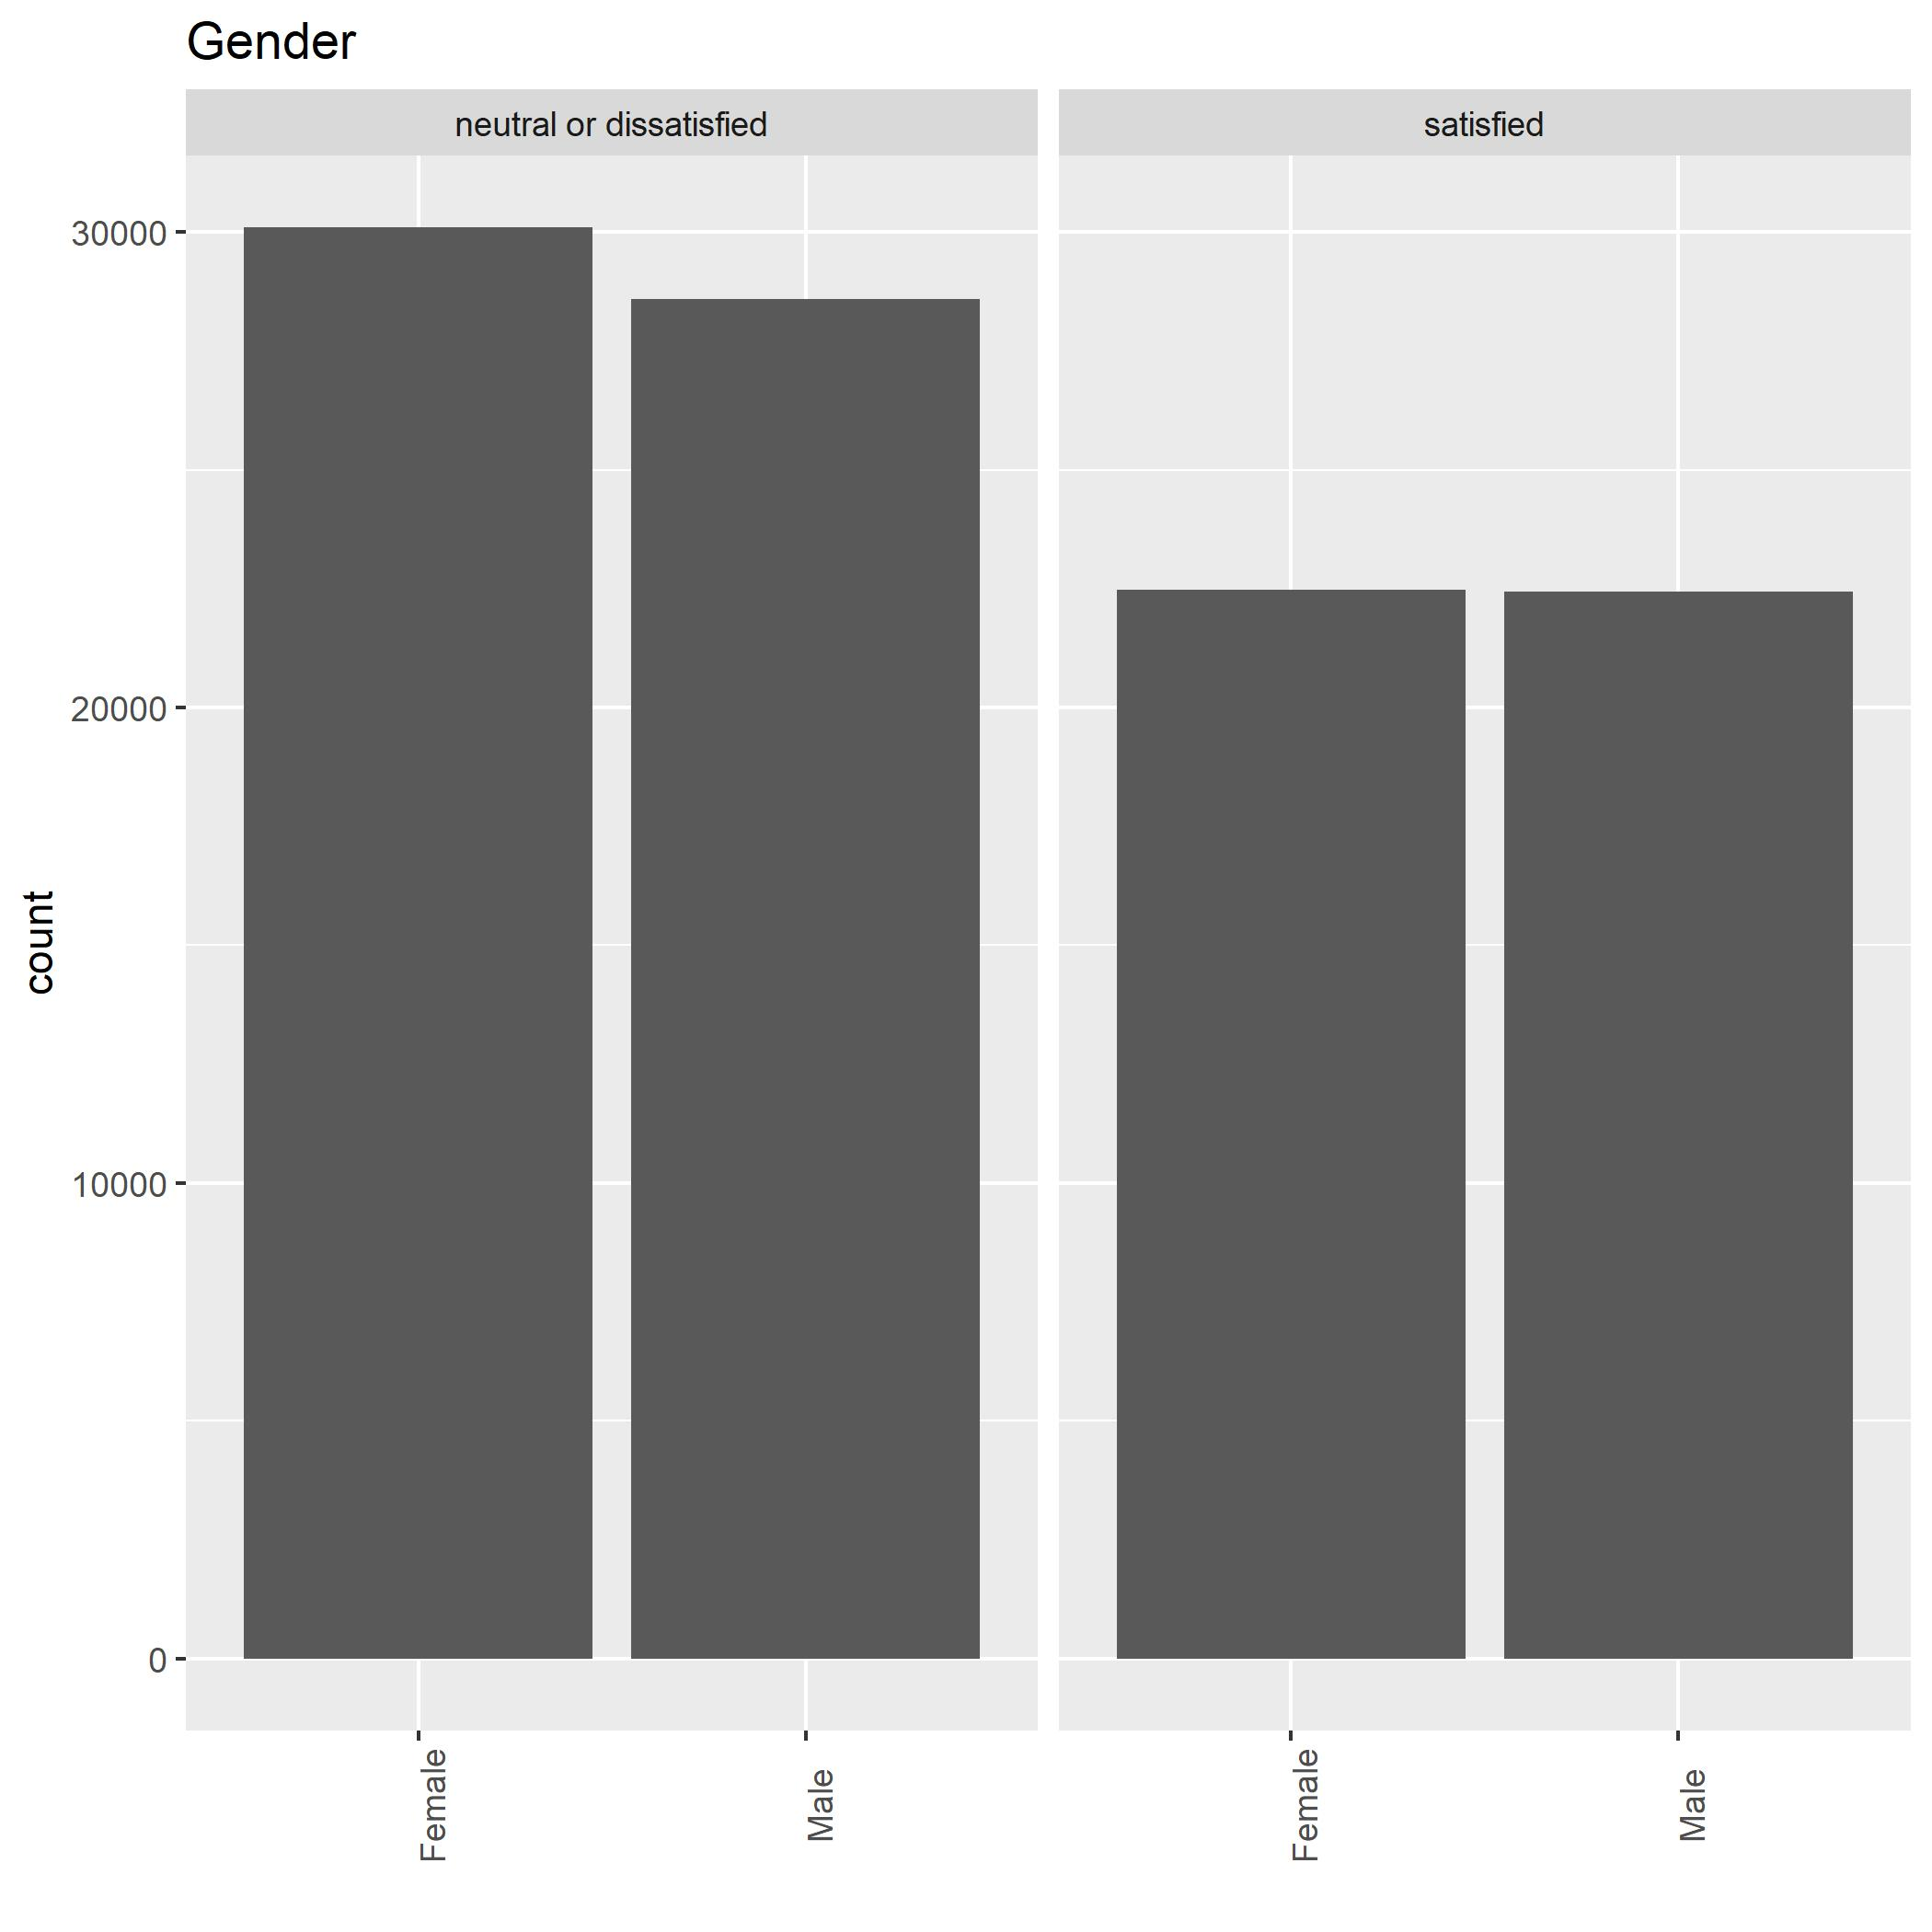
\includegraphics[width=.24\textwidth]{..//plots//plot1.jpg}\hfill
    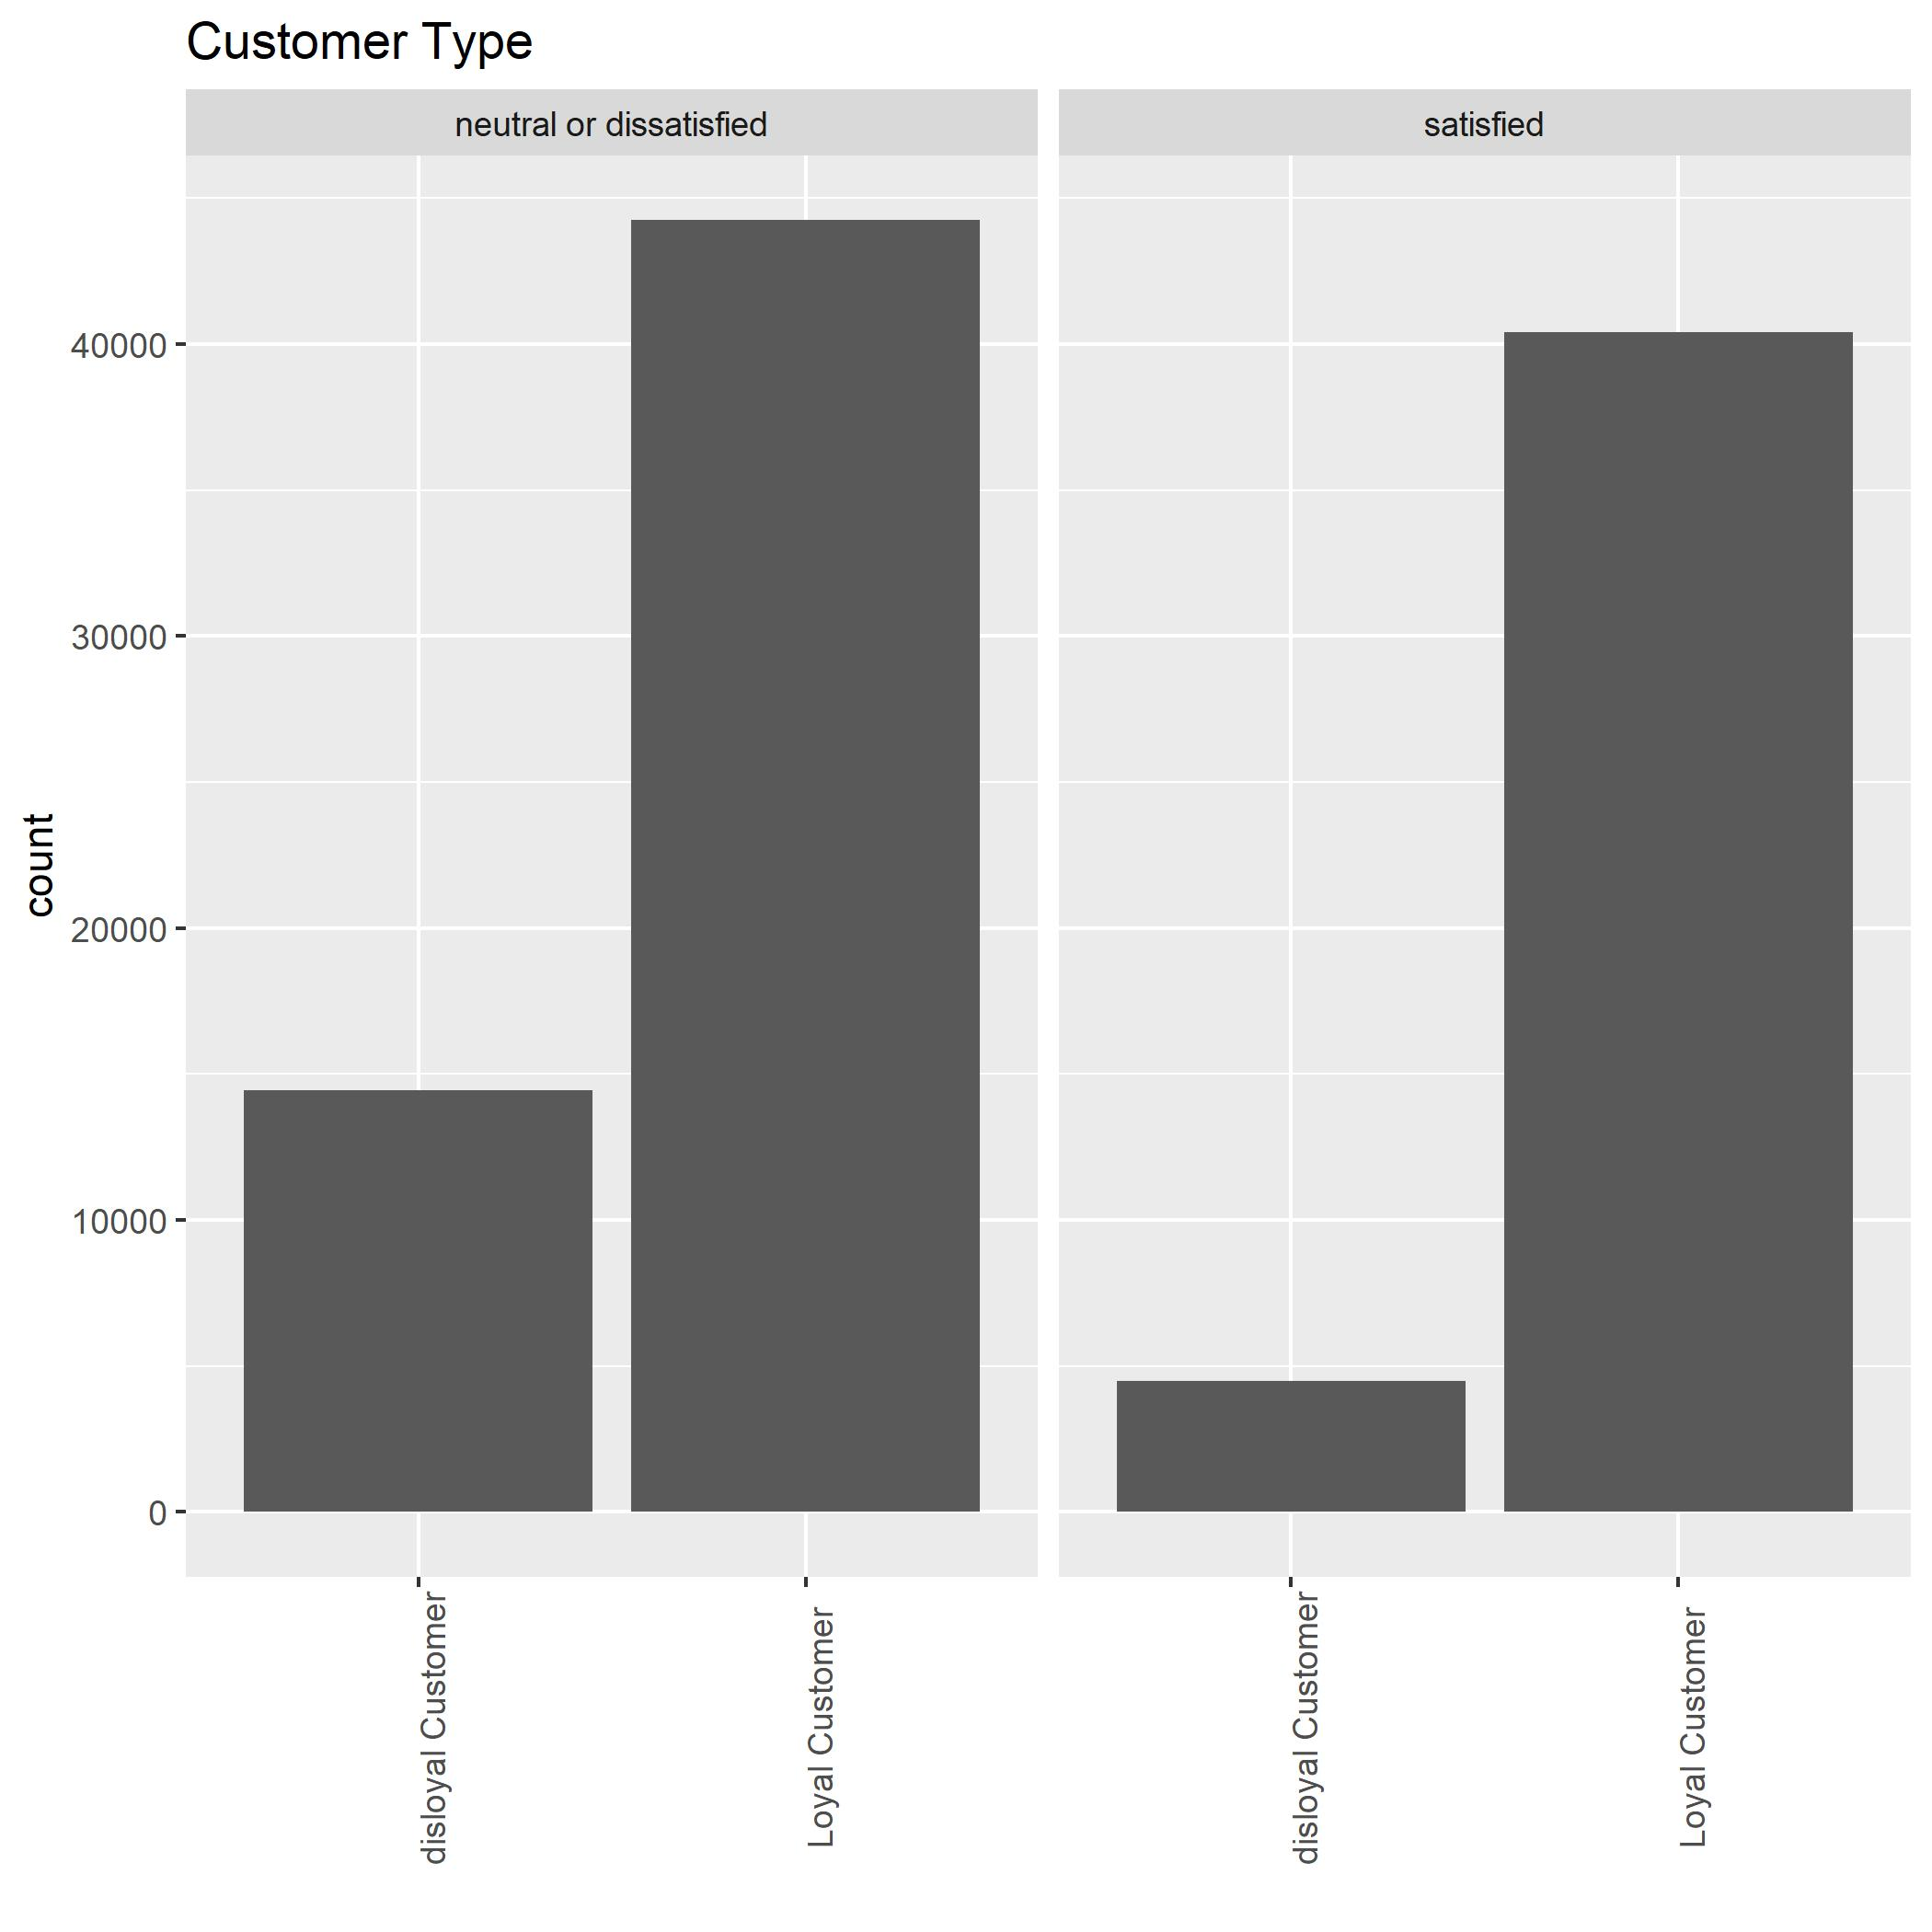
\includegraphics[width=.24\textwidth]{..//plots//plot2.jpg}\hfill
    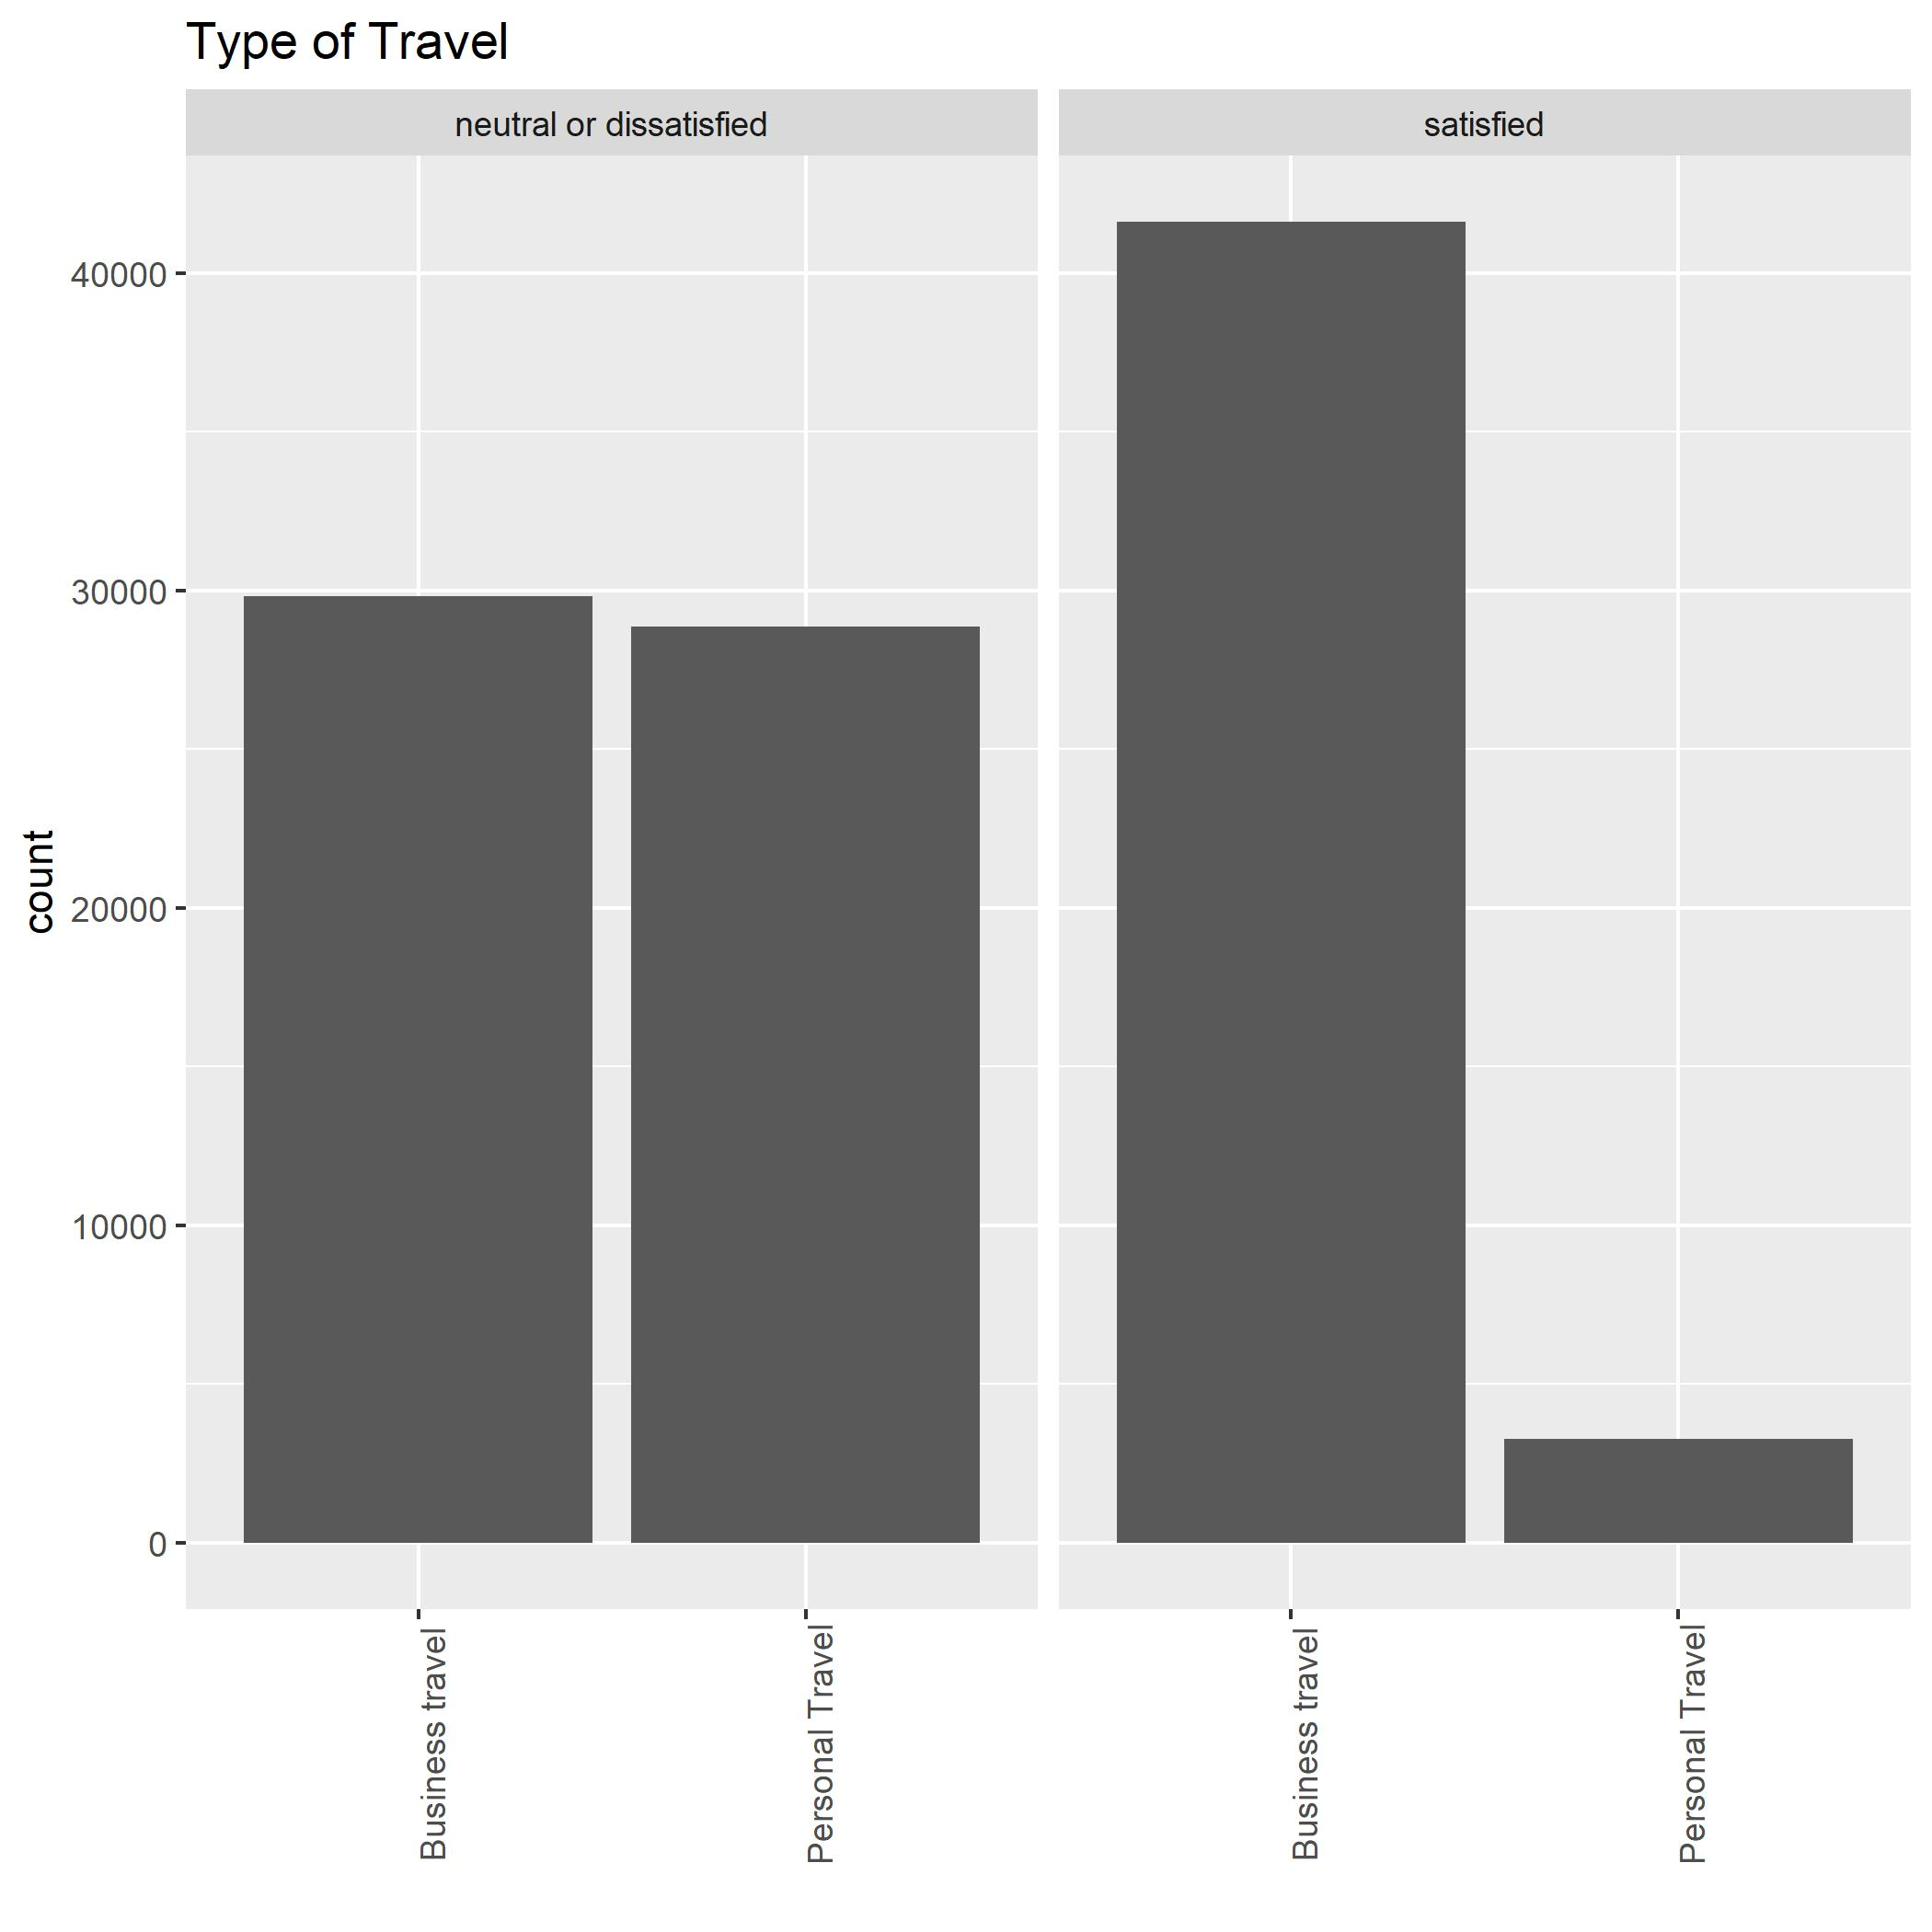
\includegraphics[width=.24\textwidth]{..//plots//plot4.jpg}\hfill
    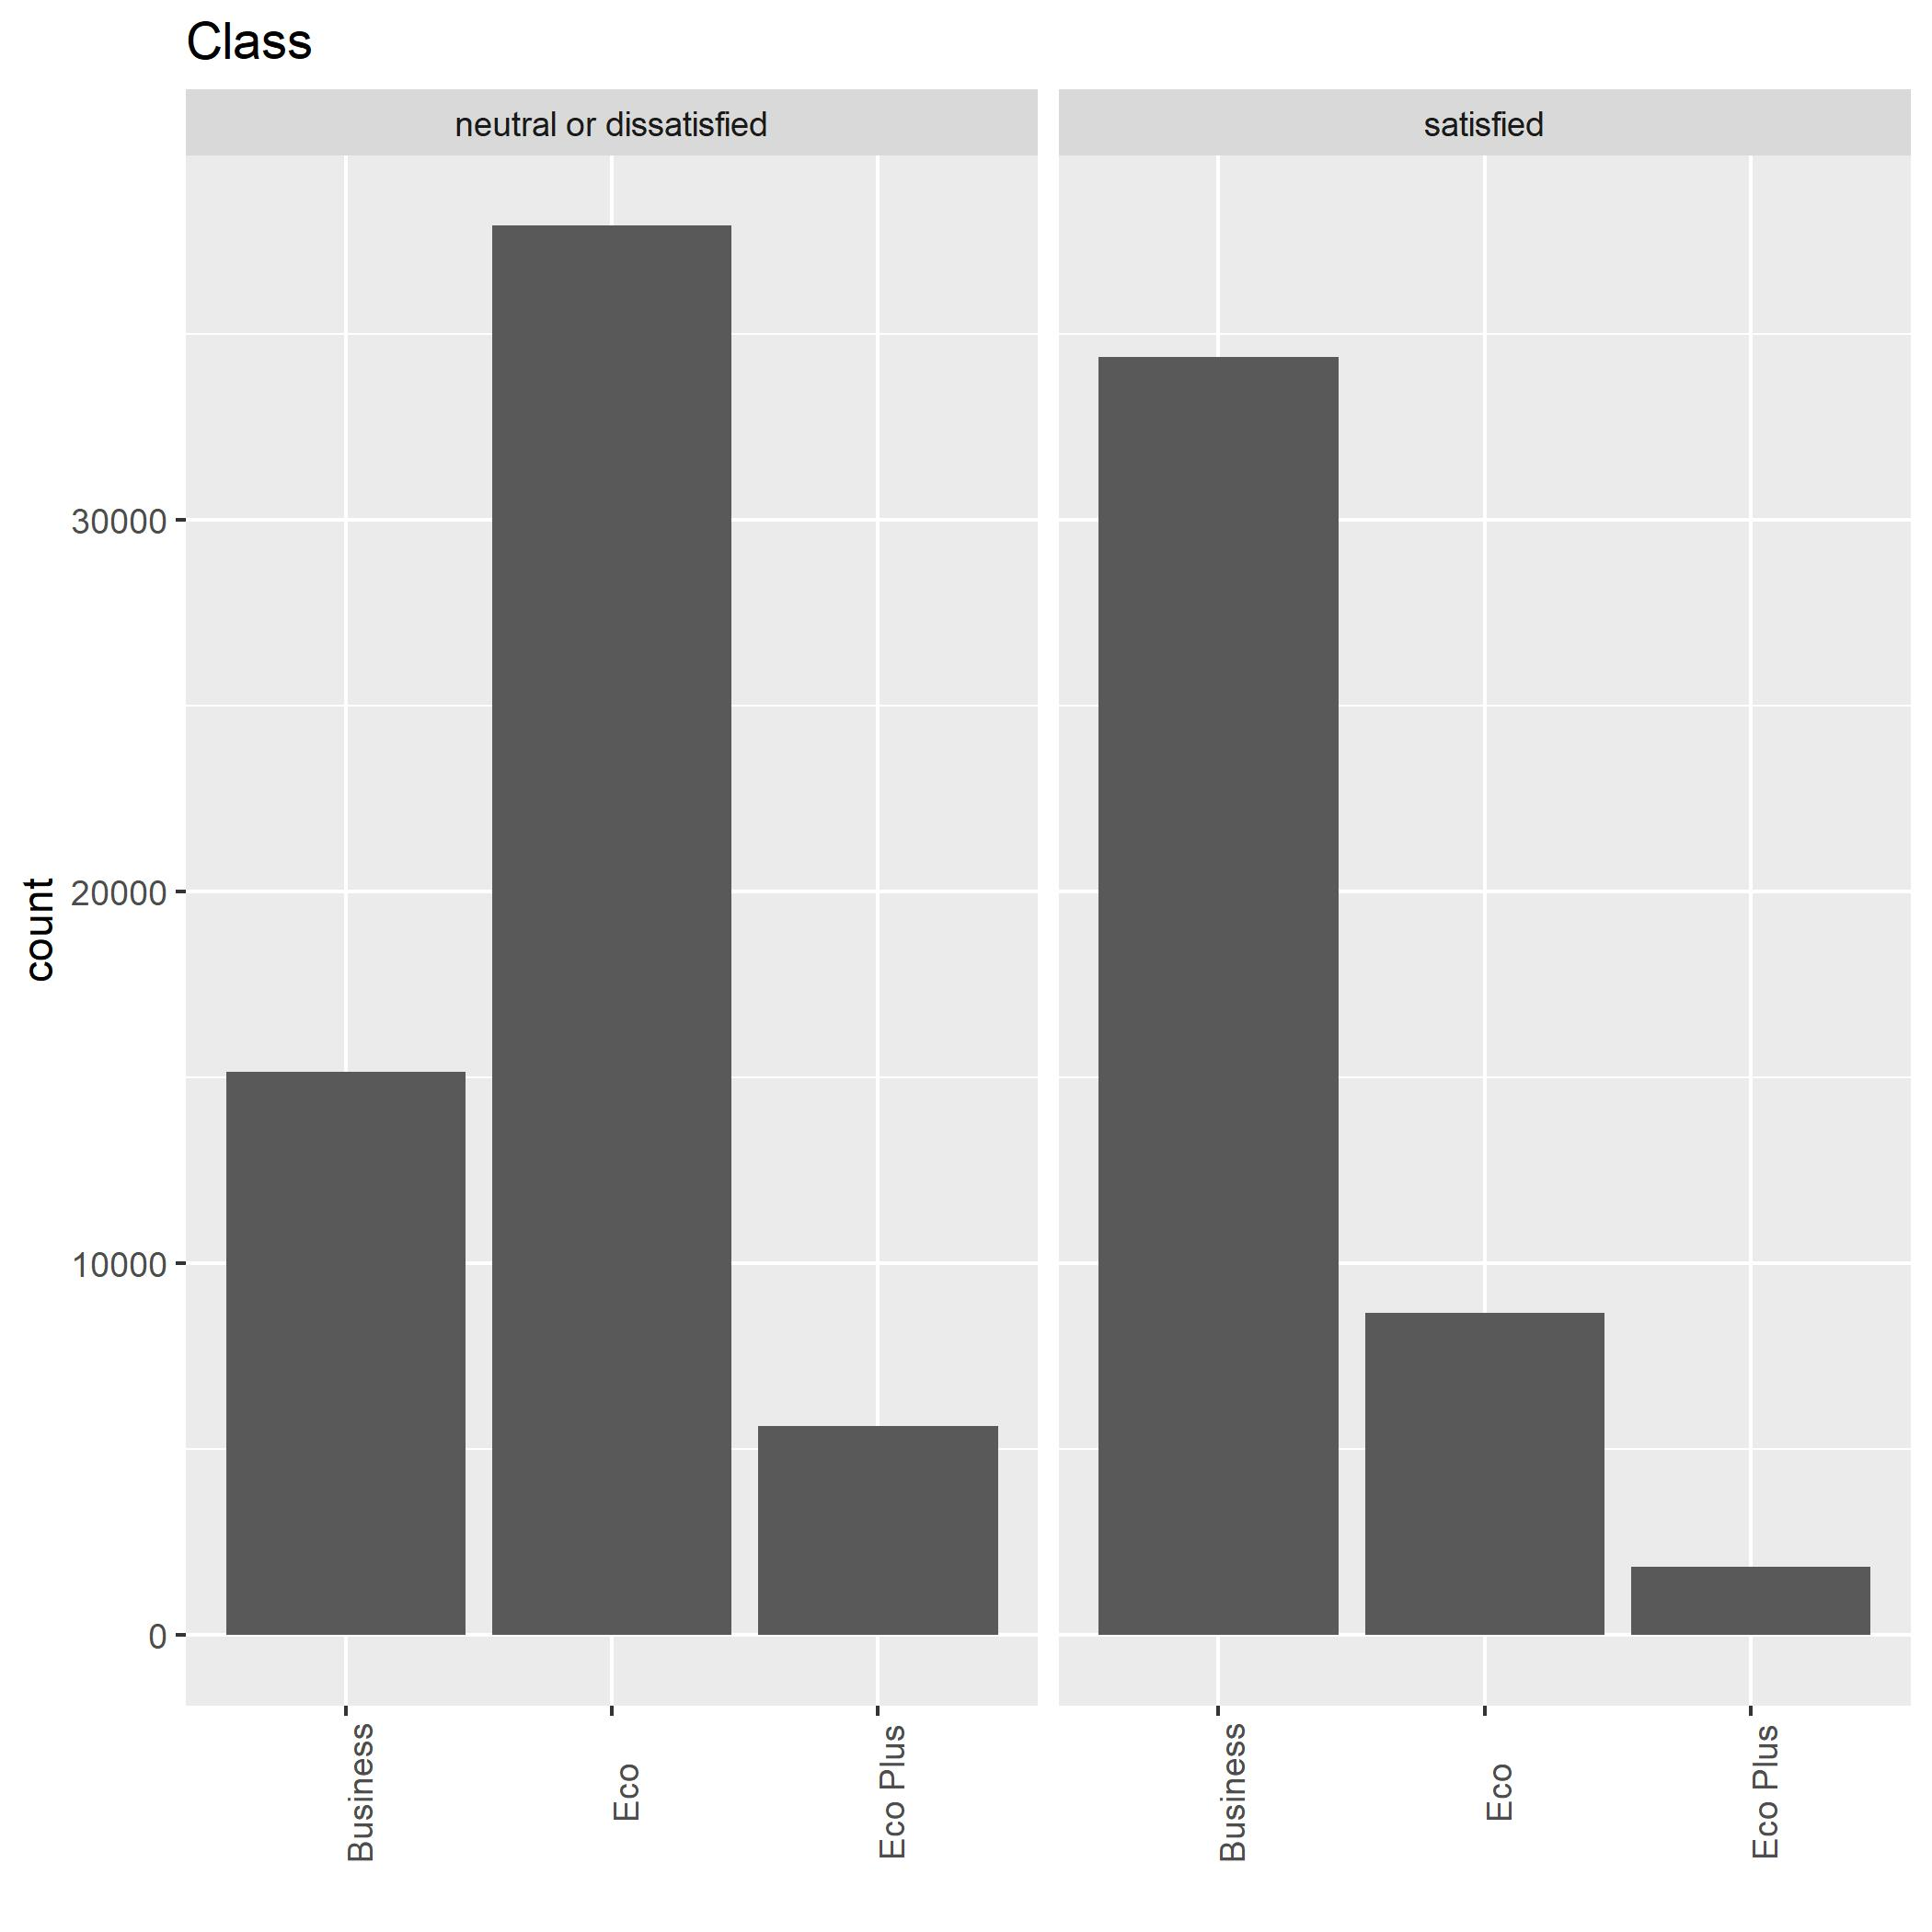
\includegraphics[width=.24\textwidth]{..//plots//plot5.jpg}\hfill
    \caption{Vizualisation of all nominal variables by criterion}\label{fig:foobar}
\end{figure}

\begin{figure}
    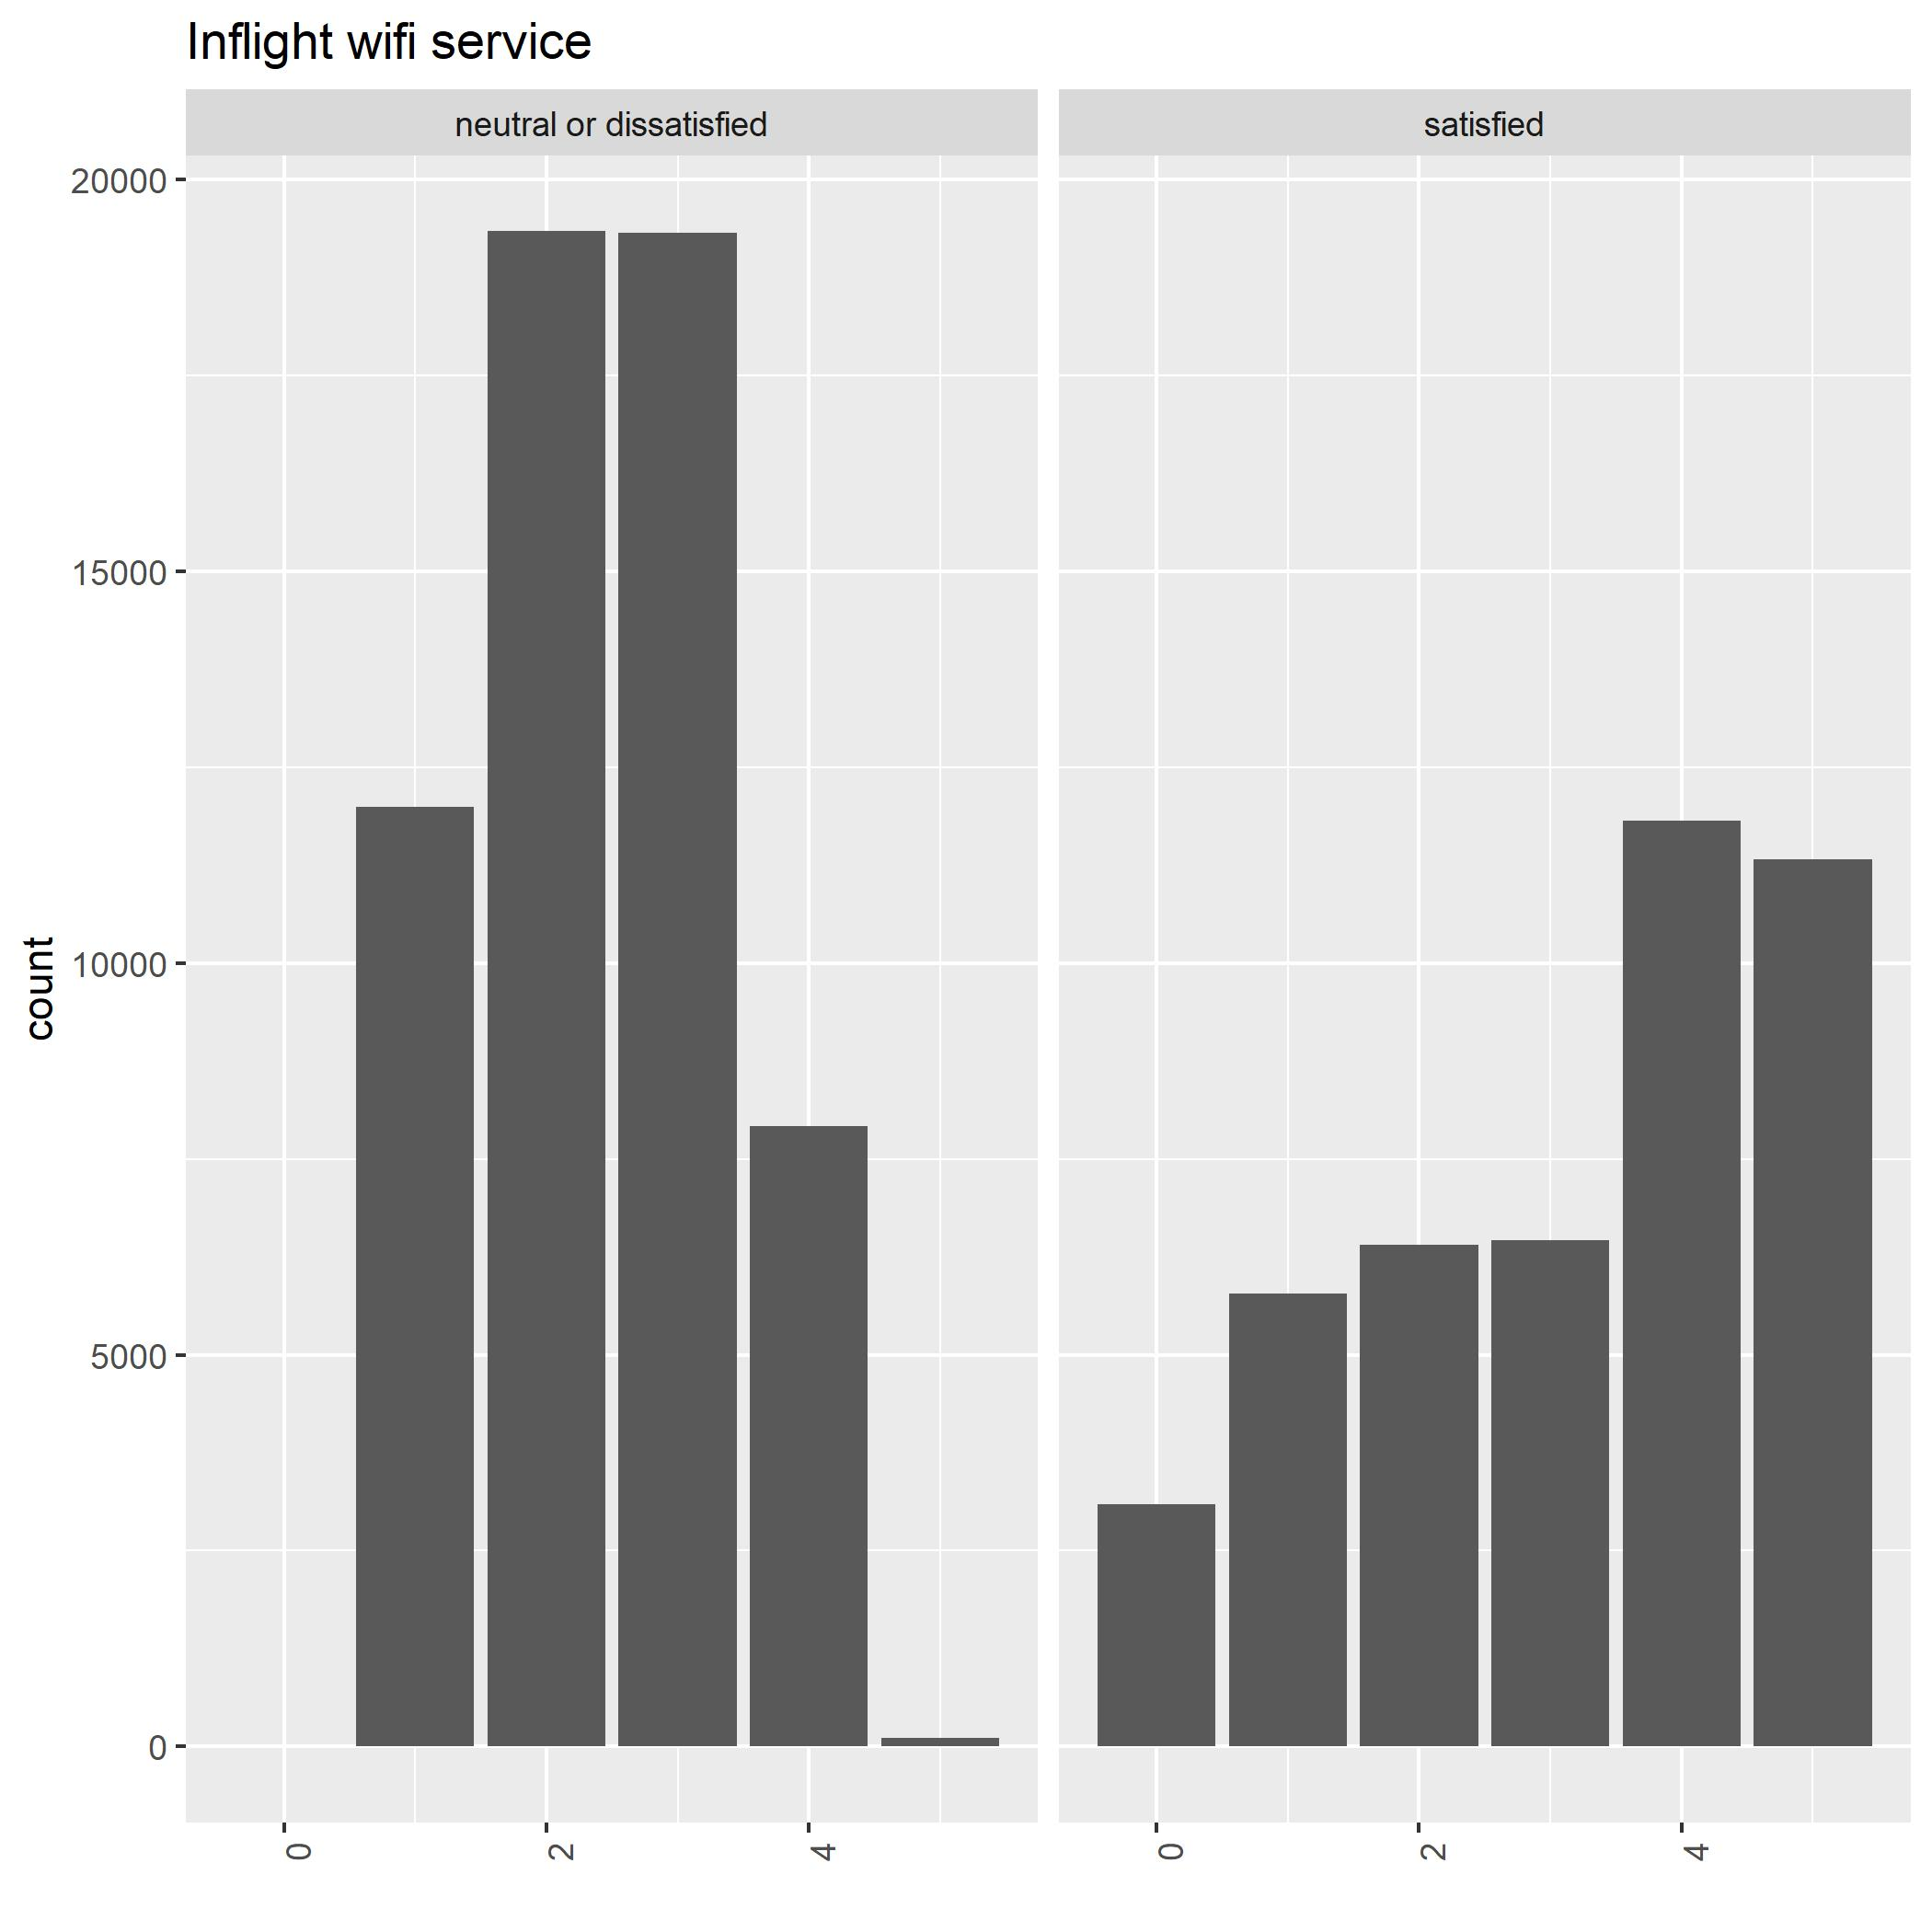
\includegraphics[width=.24\textwidth]{..//plots//plot7.jpg}\hfill
    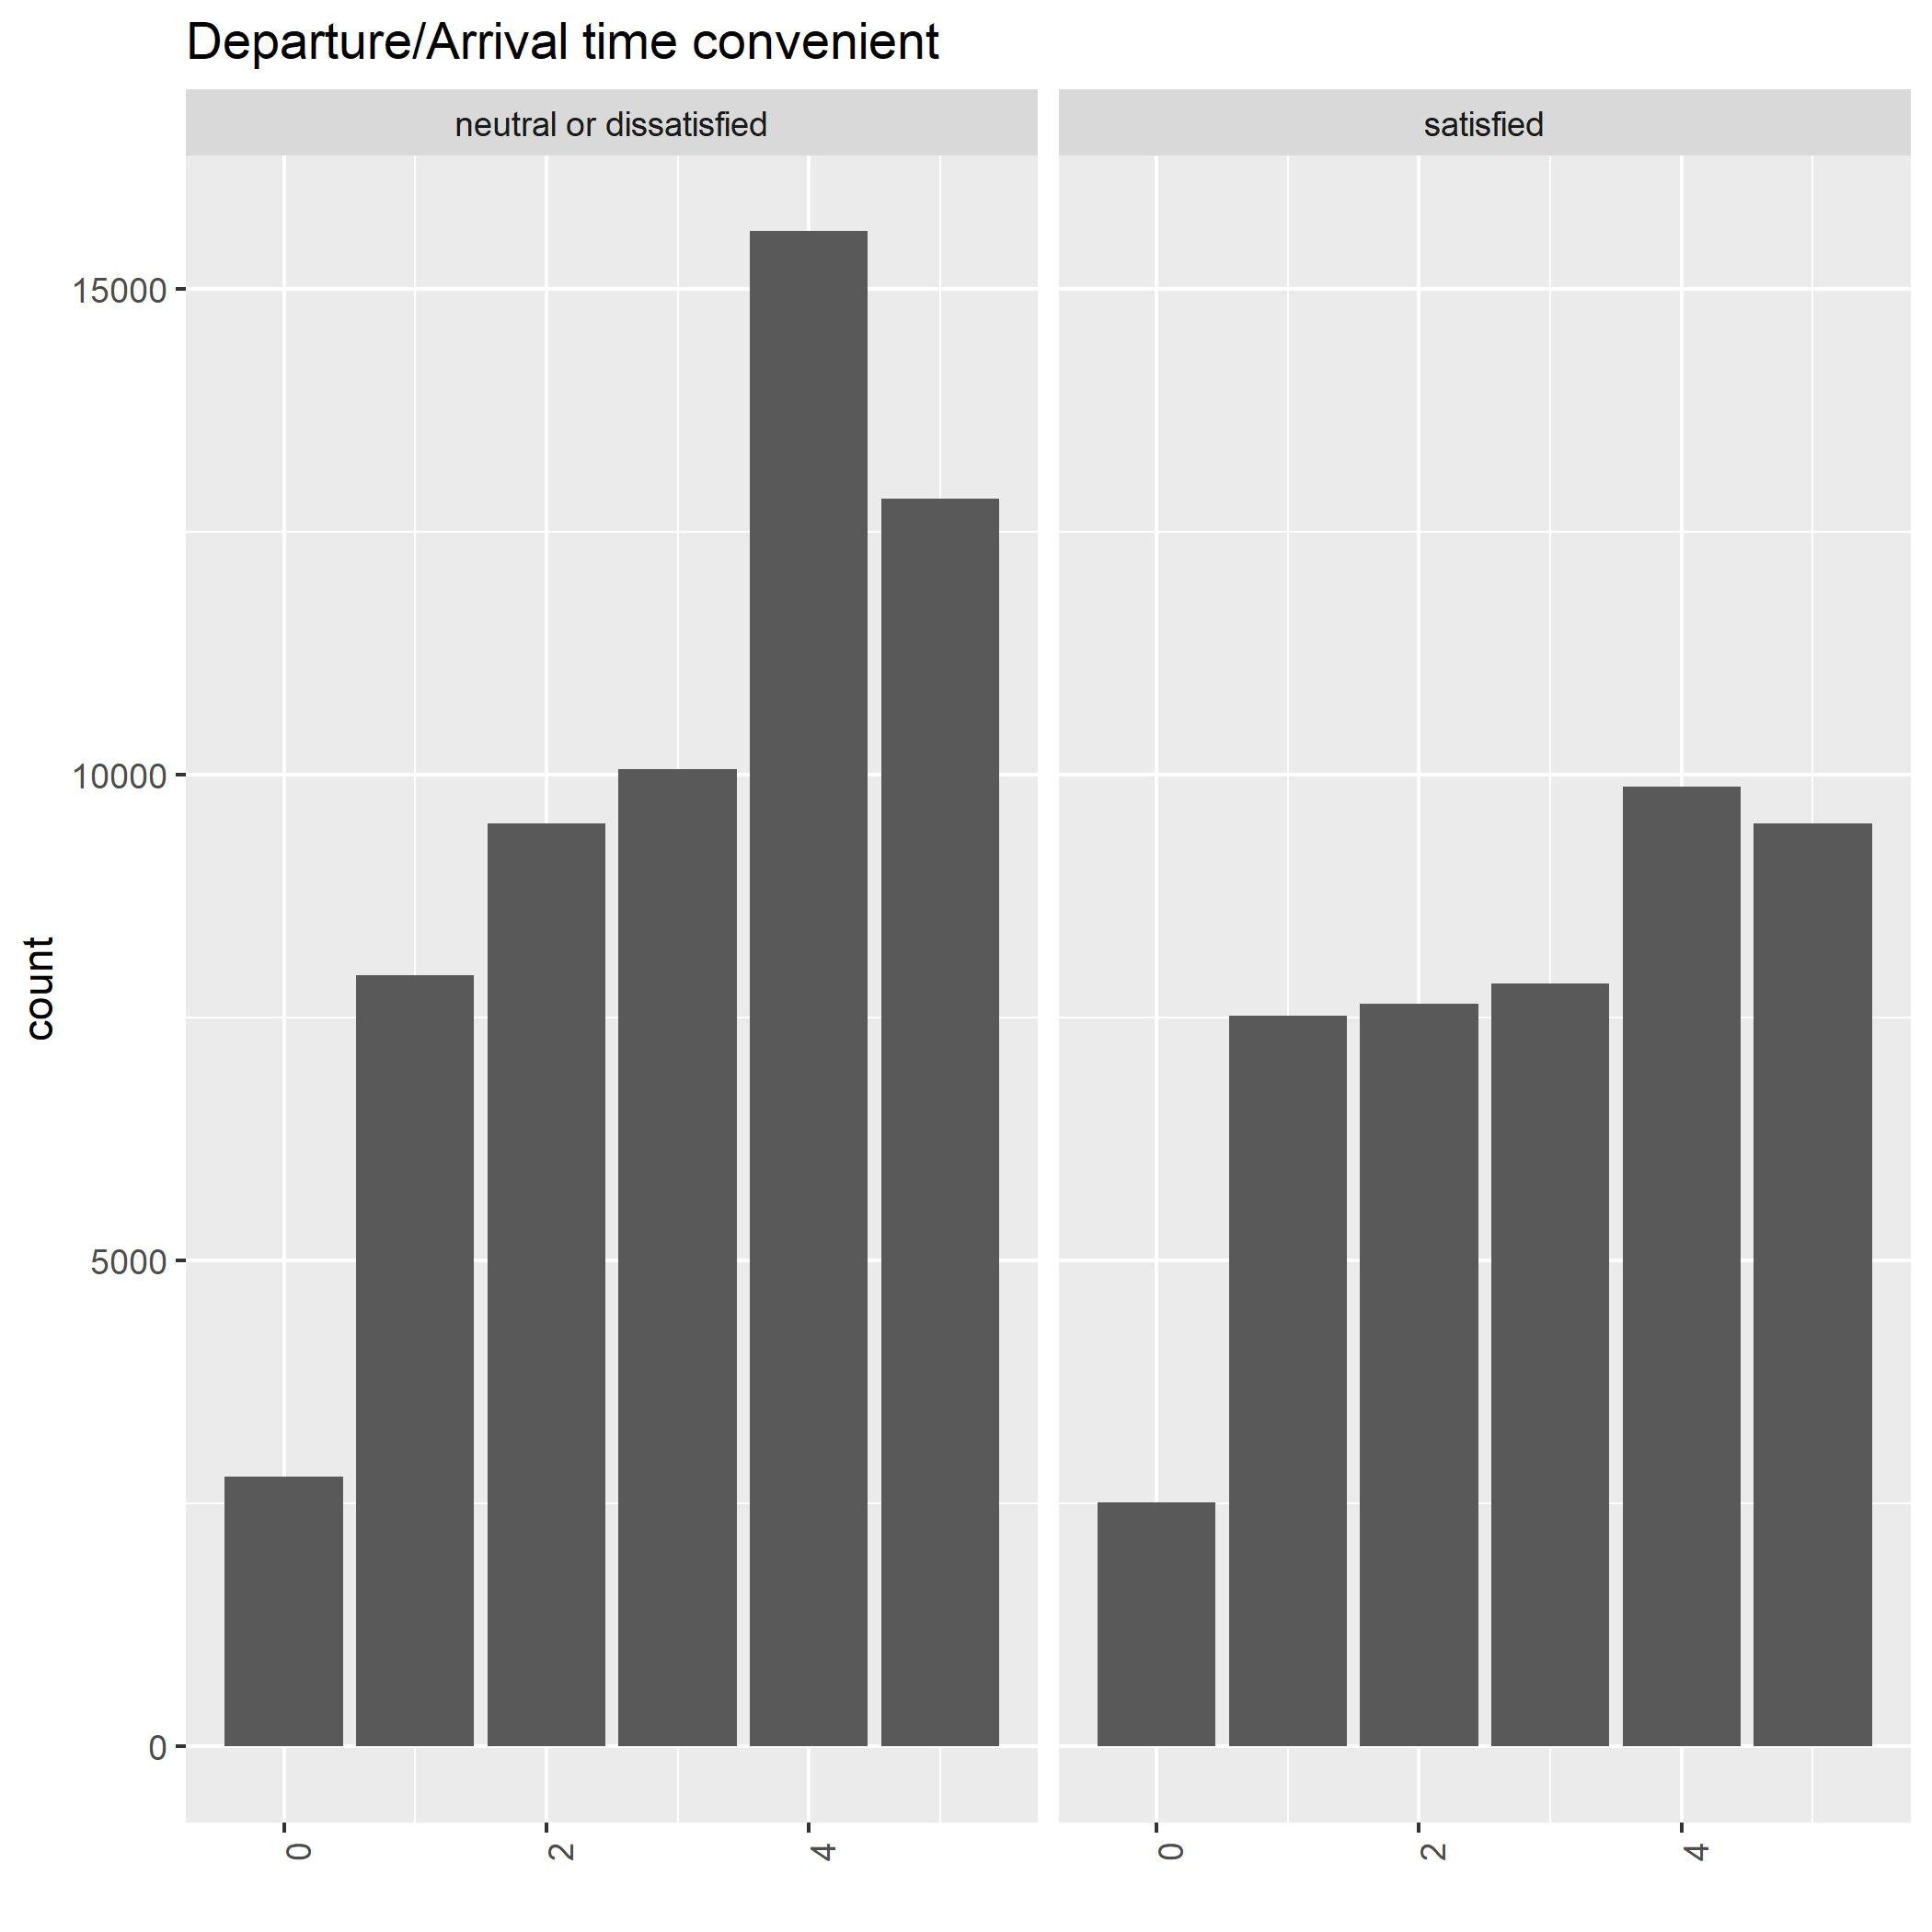
\includegraphics[width=.24\textwidth]{..//plots//plot8.jpg}\hfill
    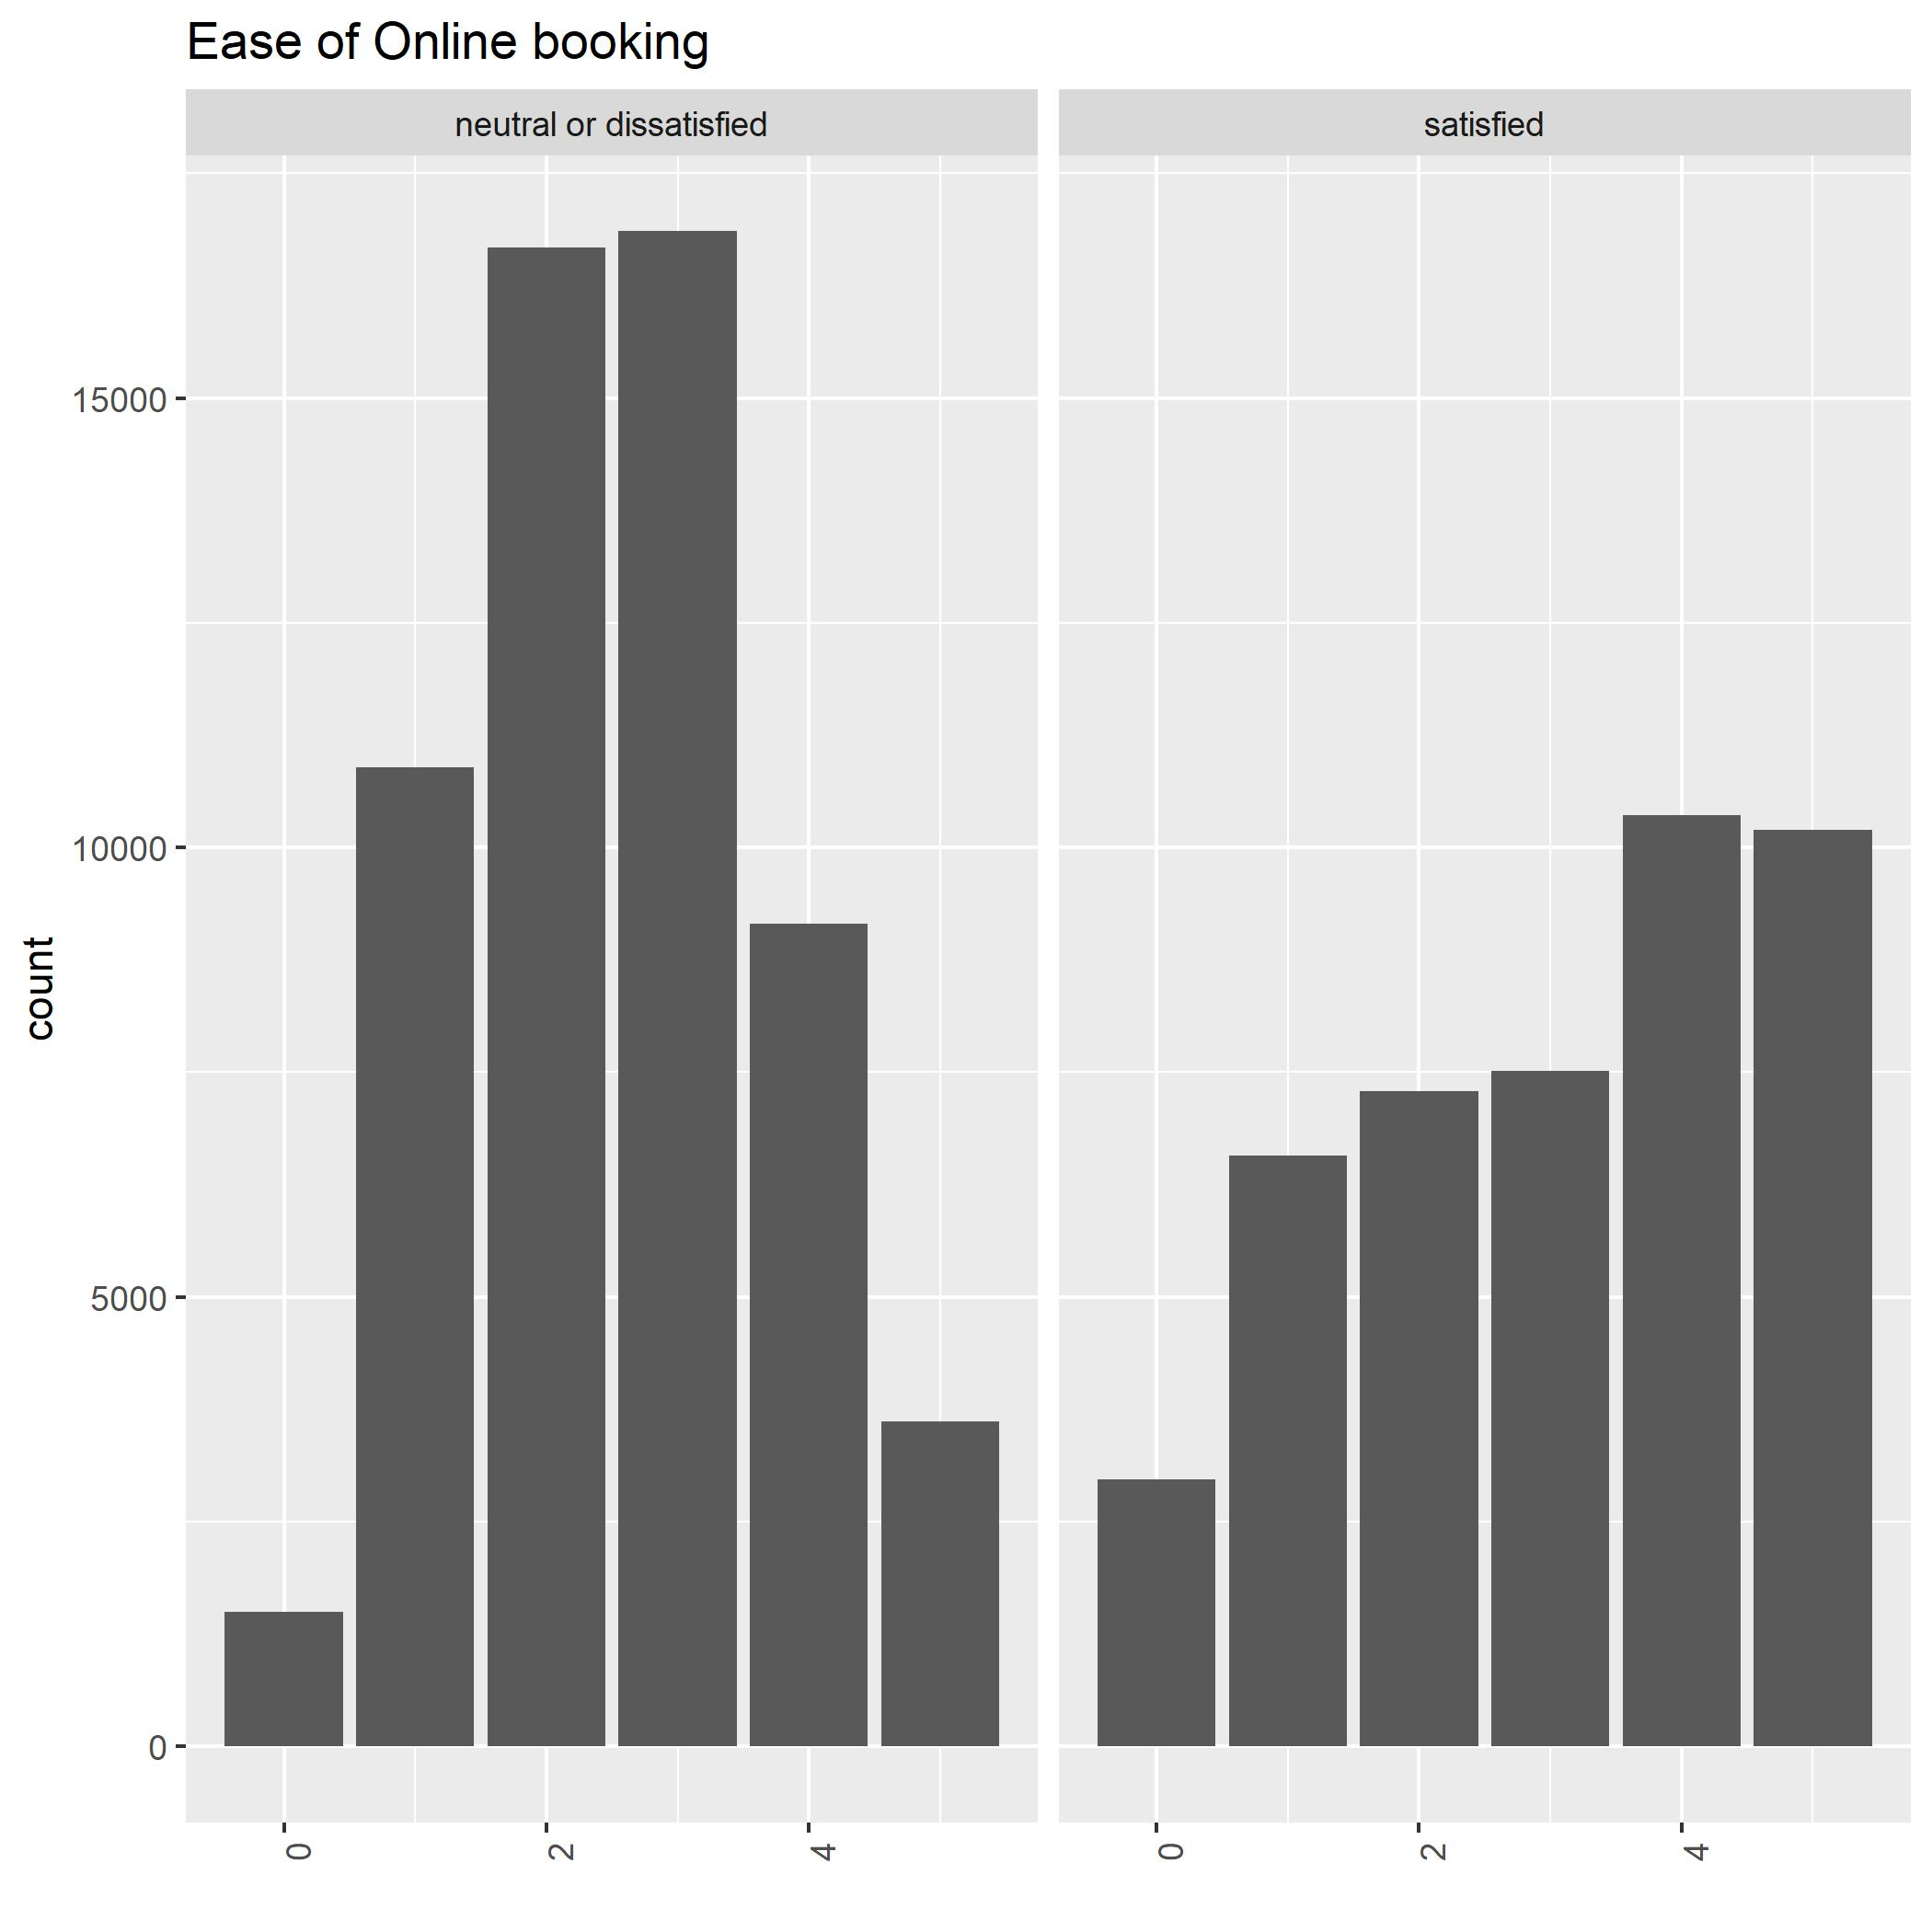
\includegraphics[width=.24\textwidth]{..//plots//plot9.jpg}\hfill
    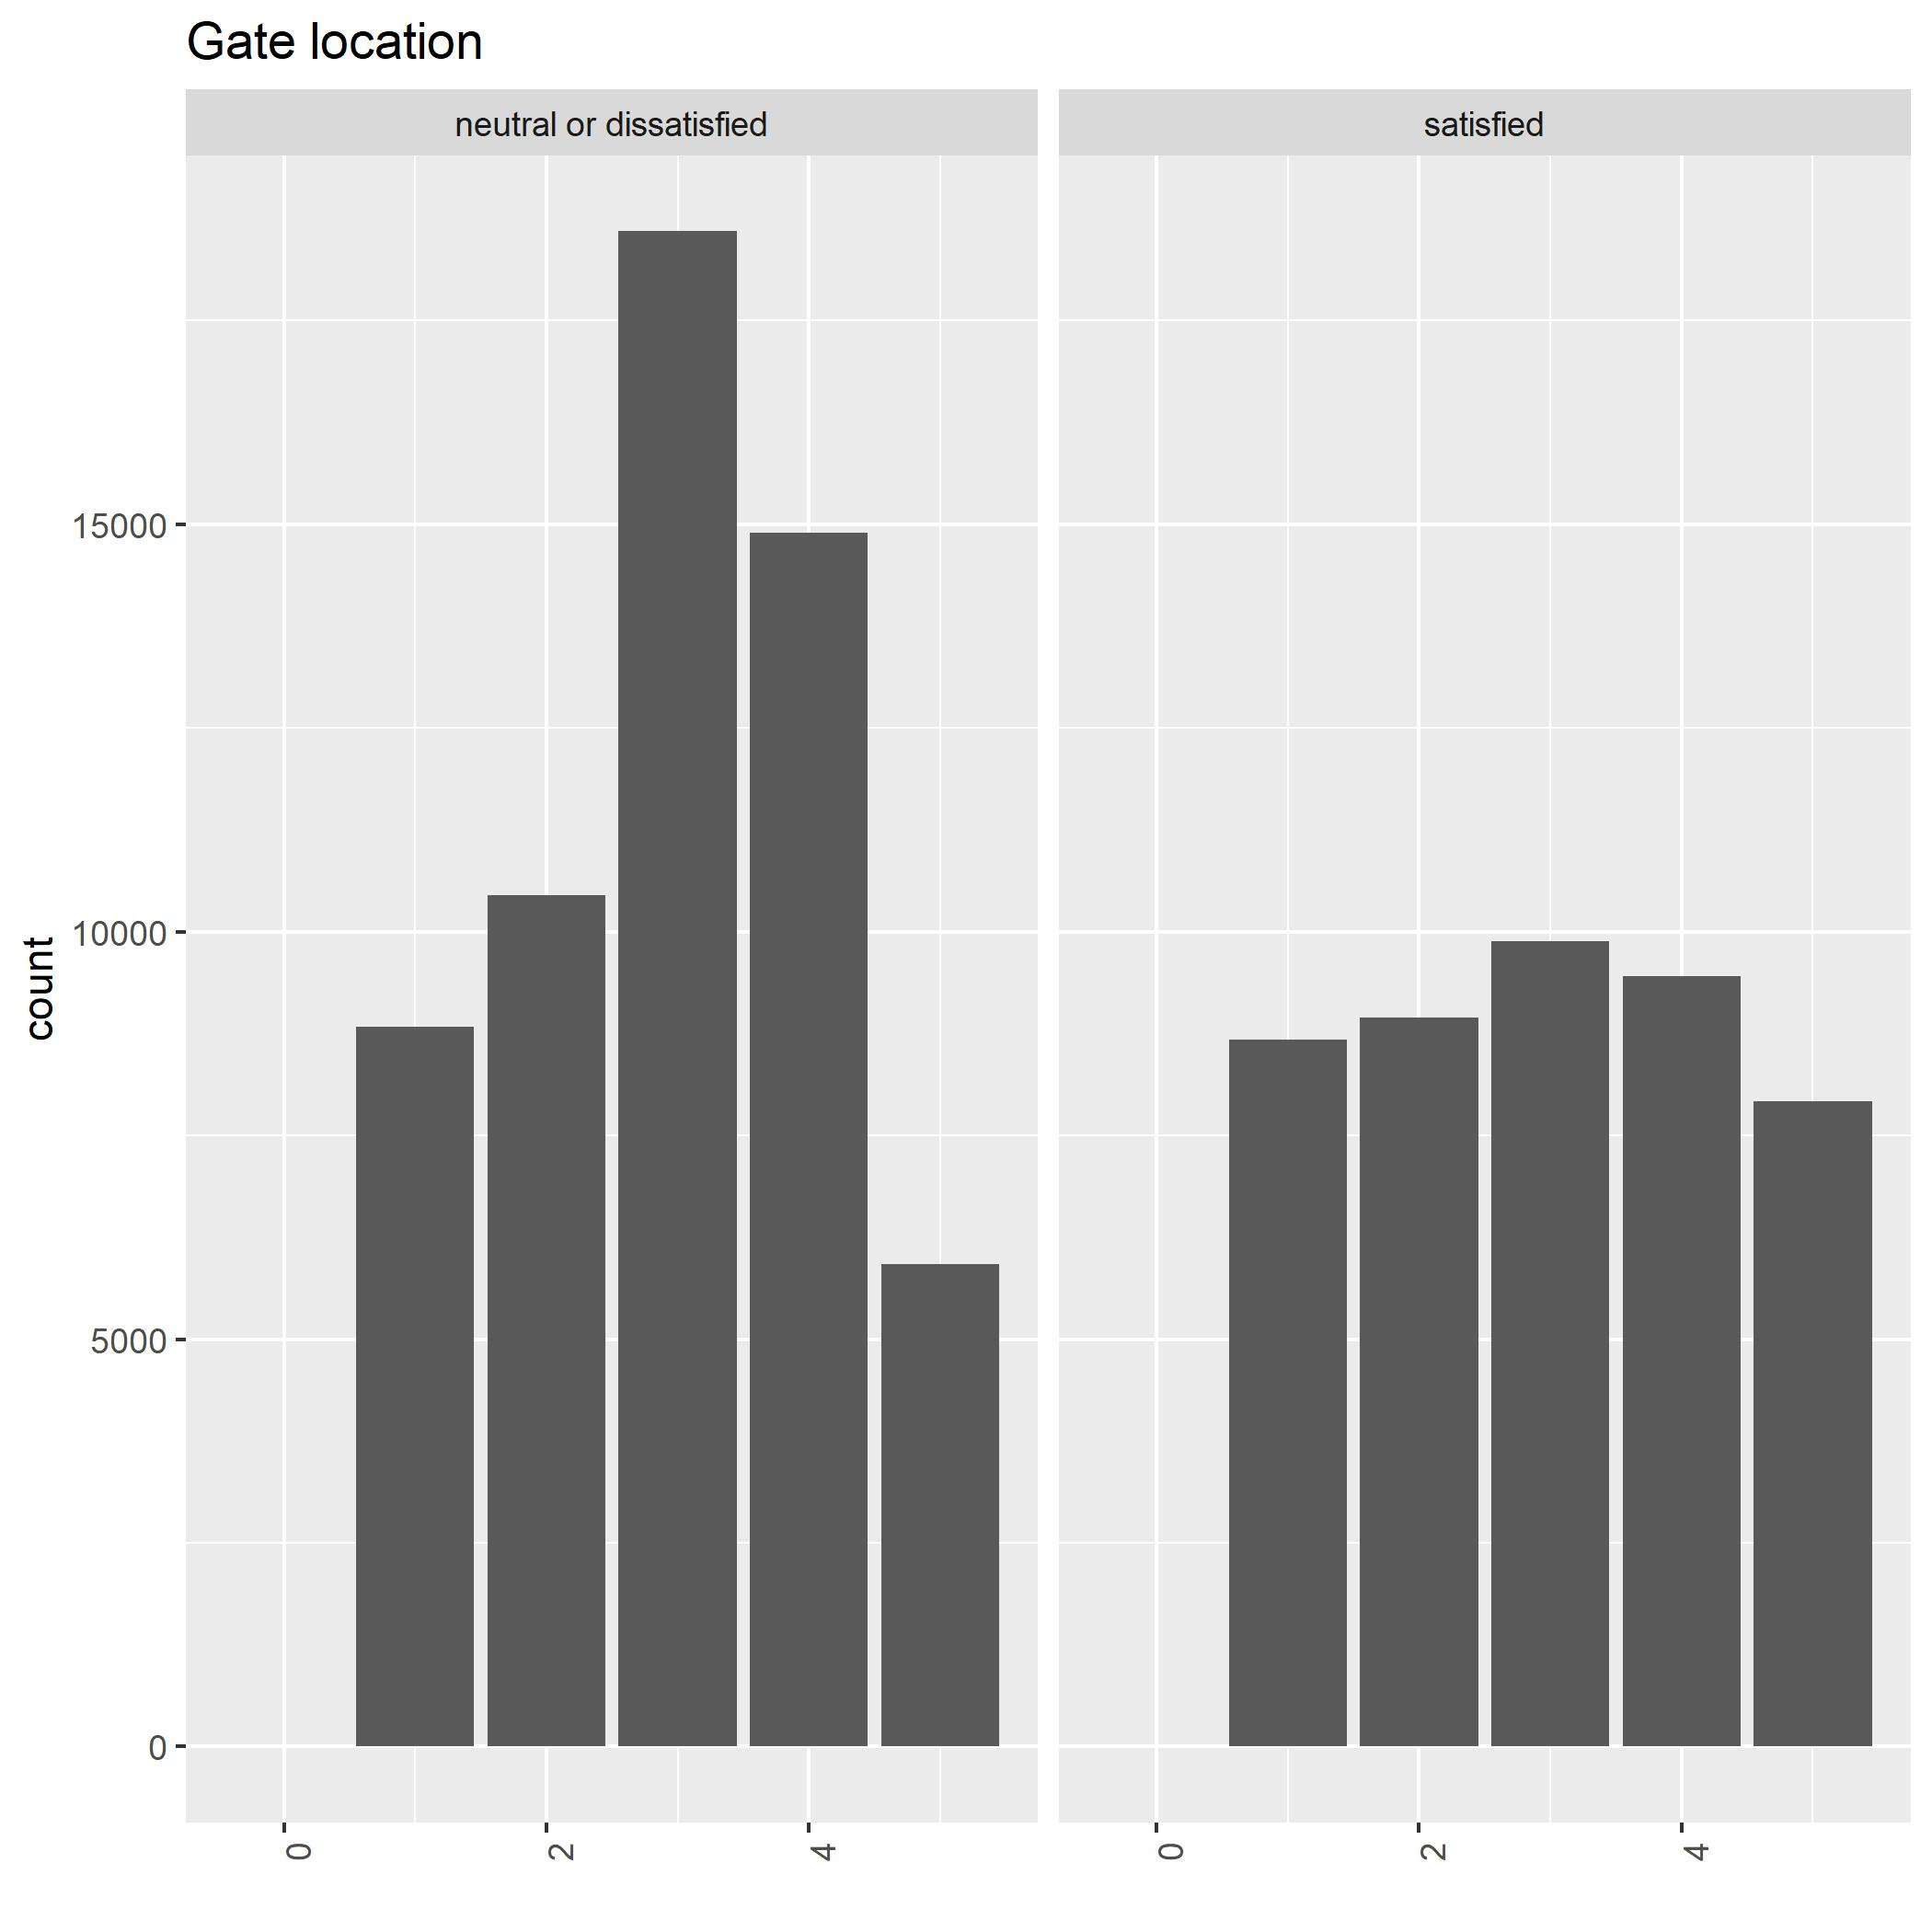
\includegraphics[width=.24\textwidth]{..//plots//plot10.jpg}\hfill
    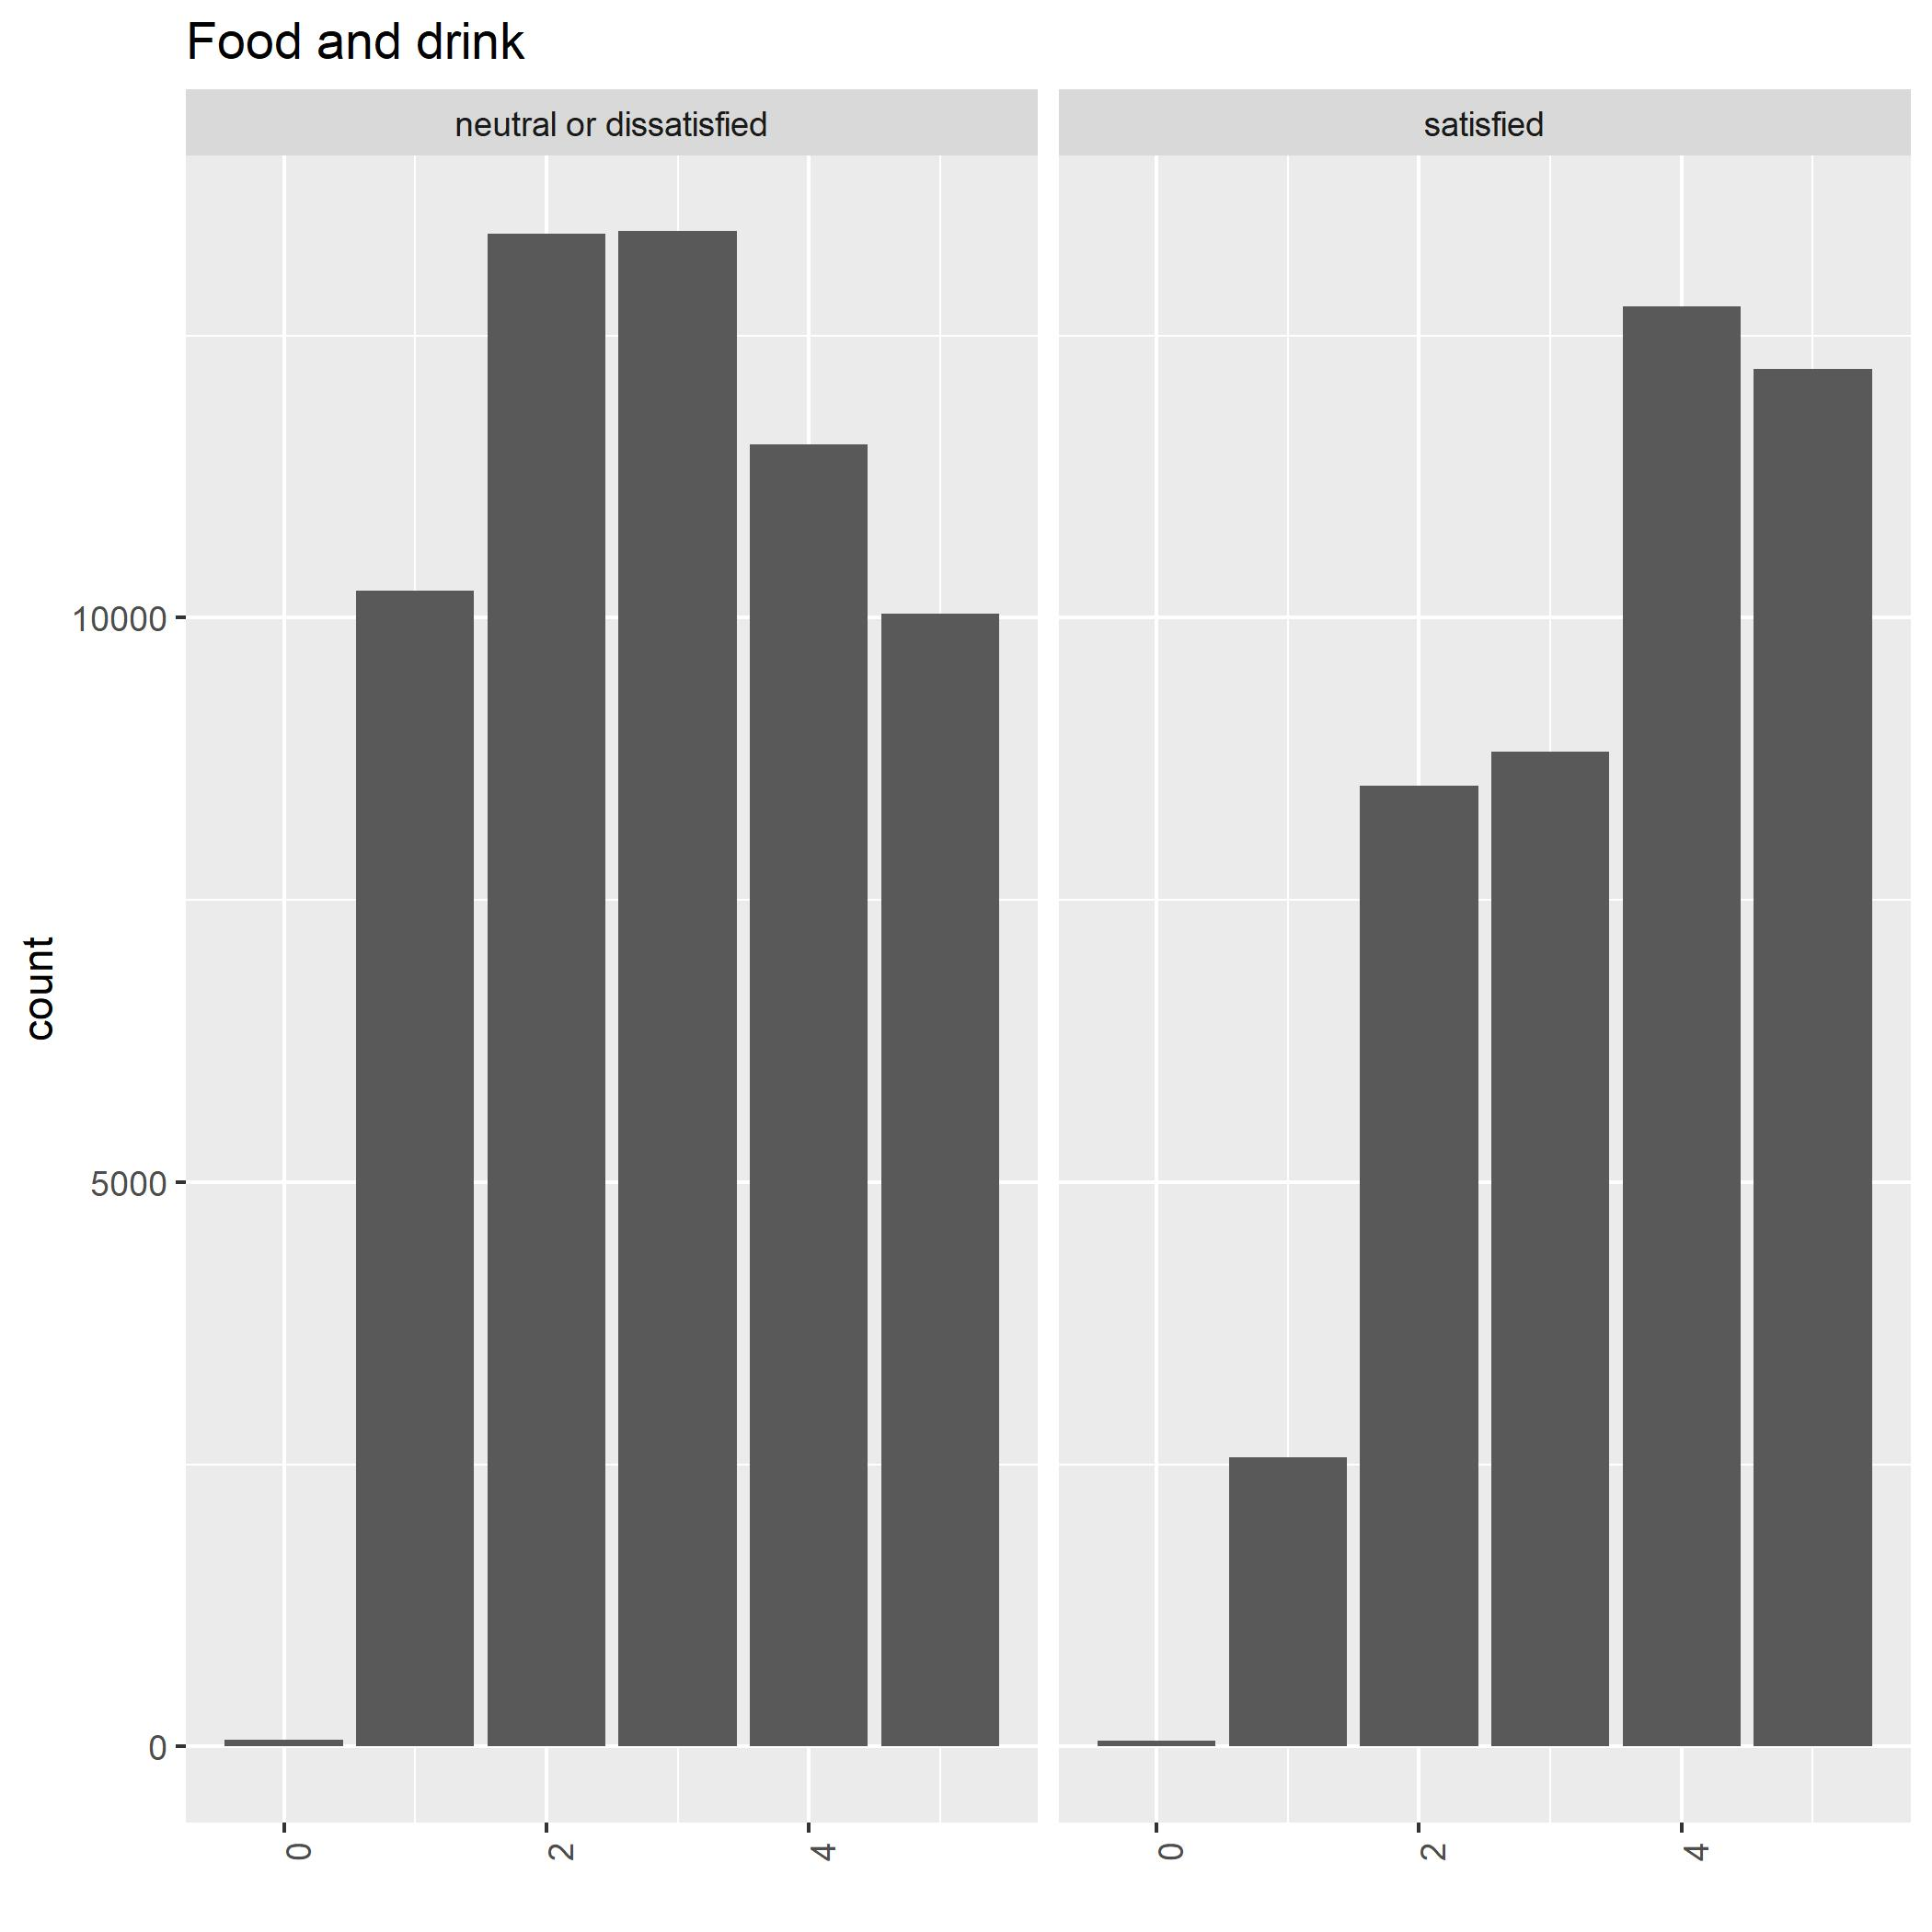
\includegraphics[width=.24\textwidth]{..//plots//plot11.jpg}\hfill
    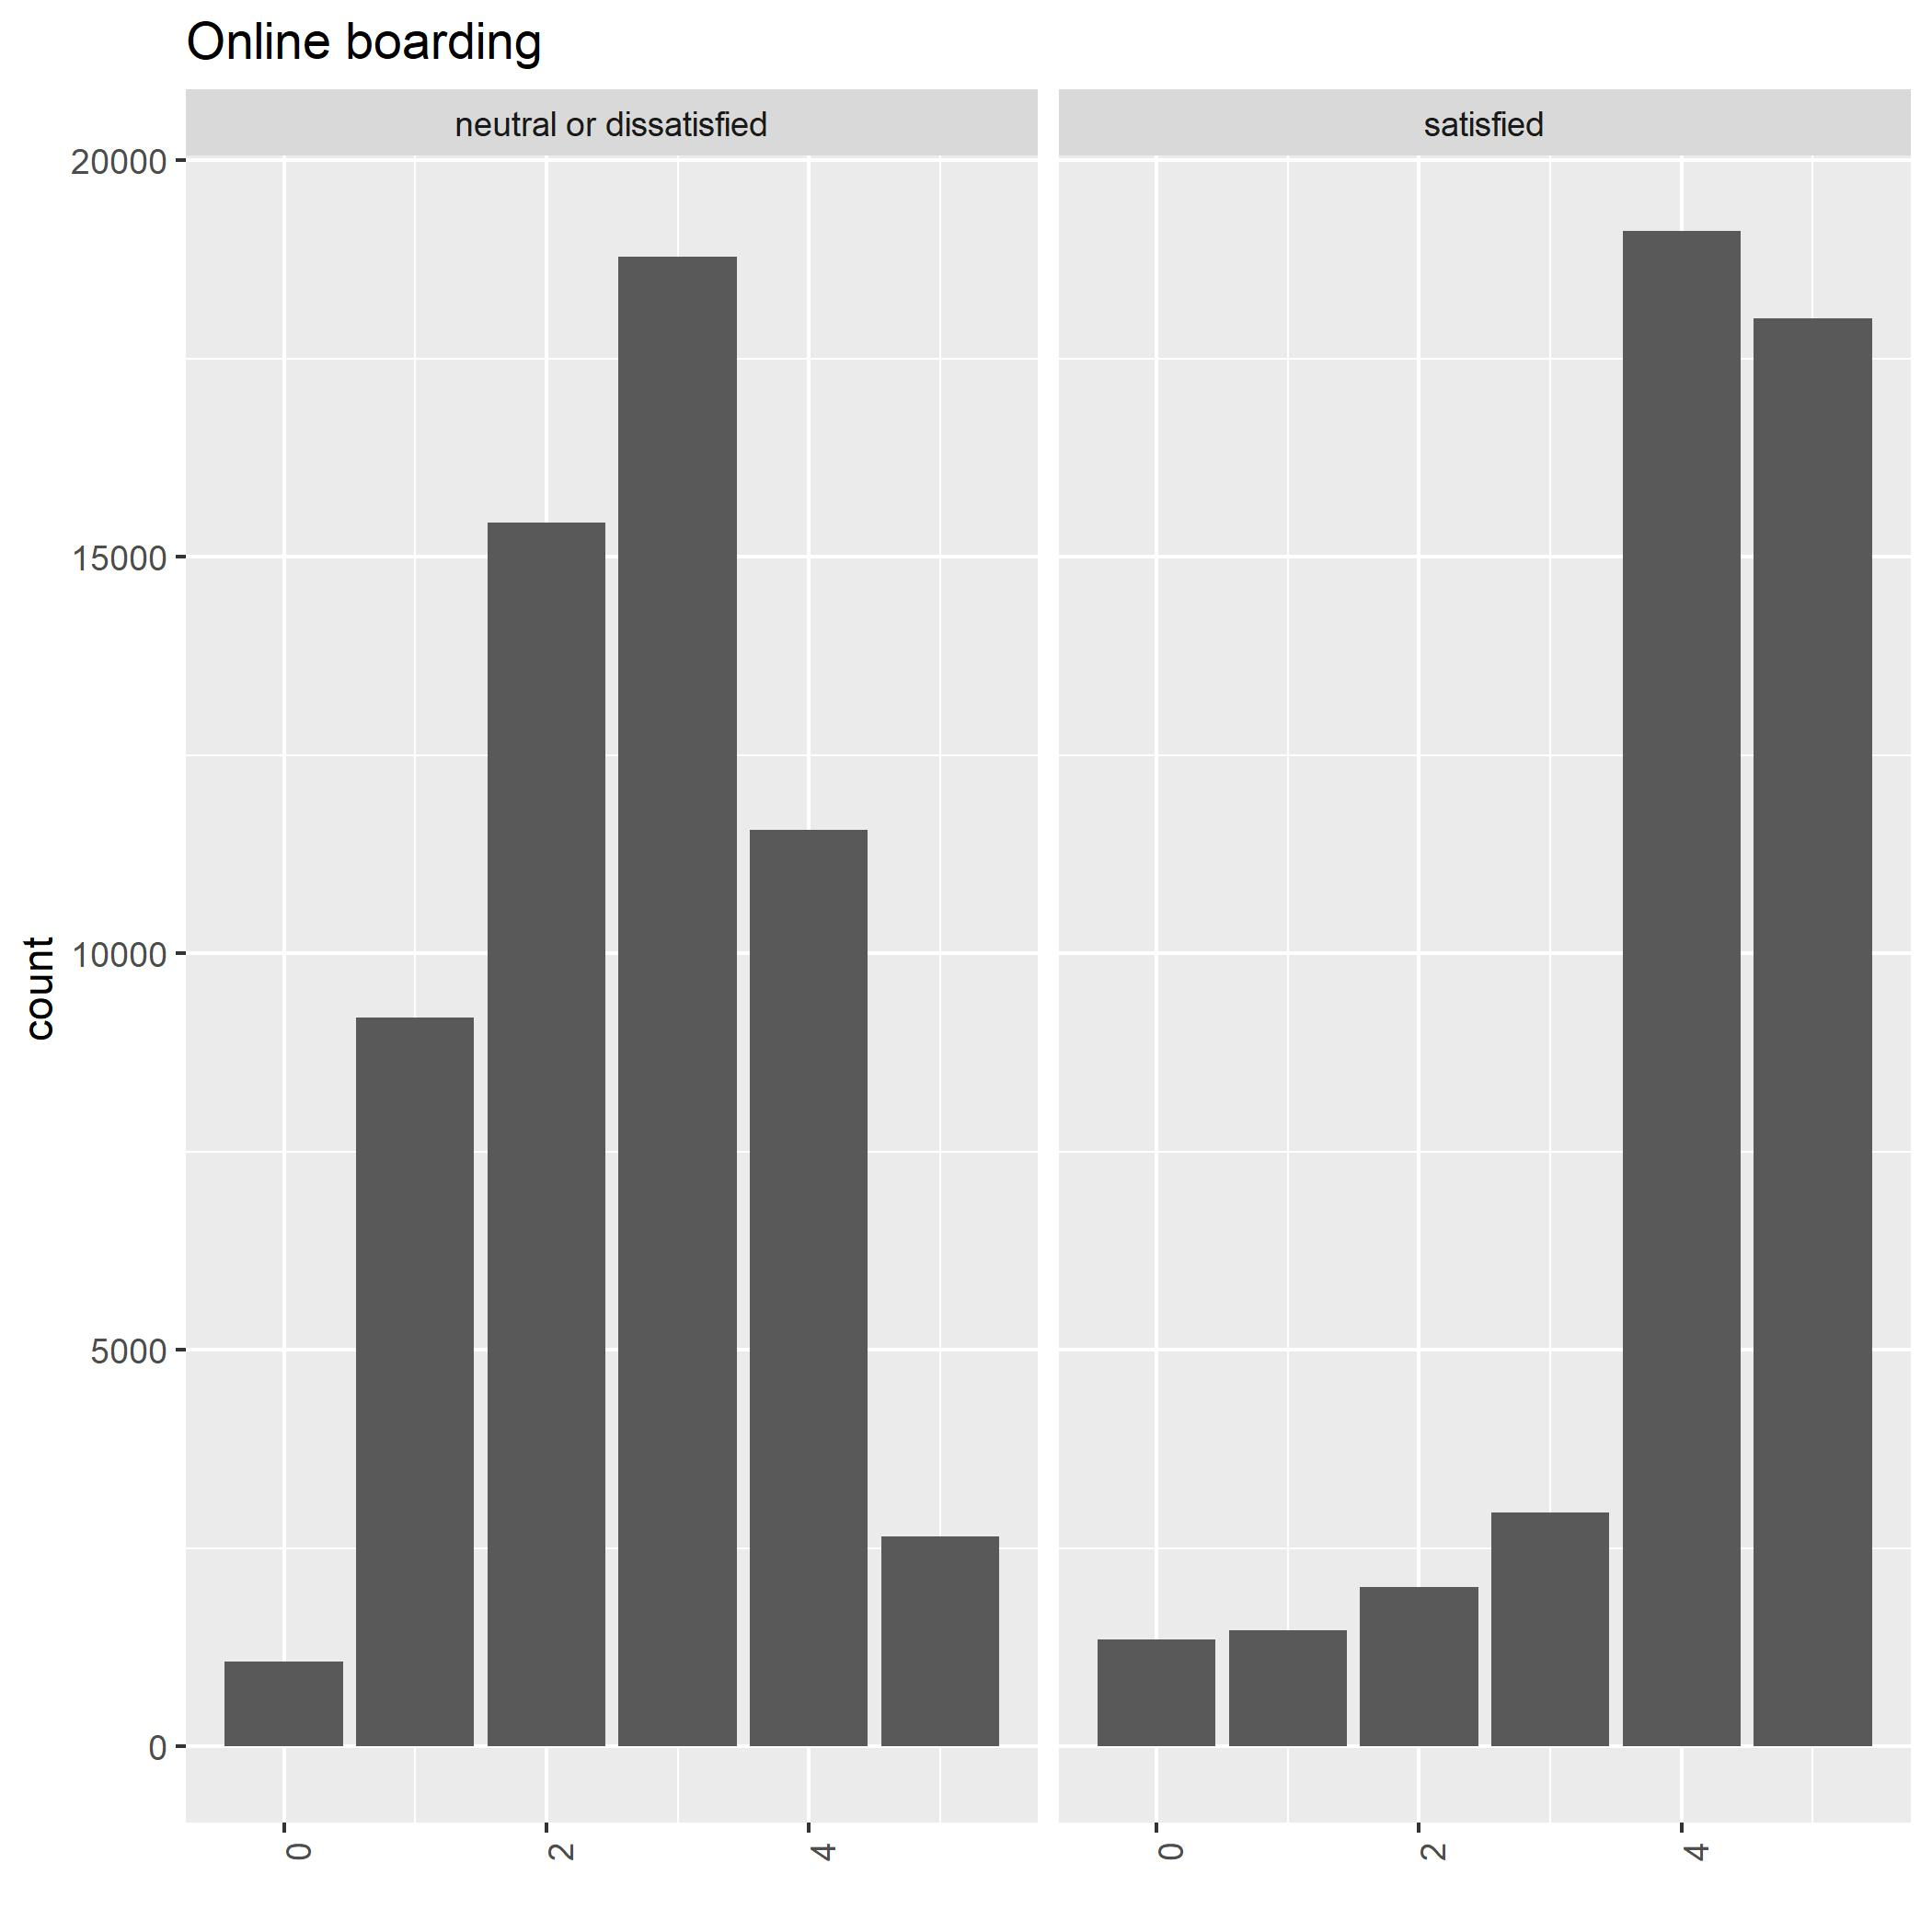
\includegraphics[width=.24\textwidth]{..//plots//plot12.jpg}\hfill
    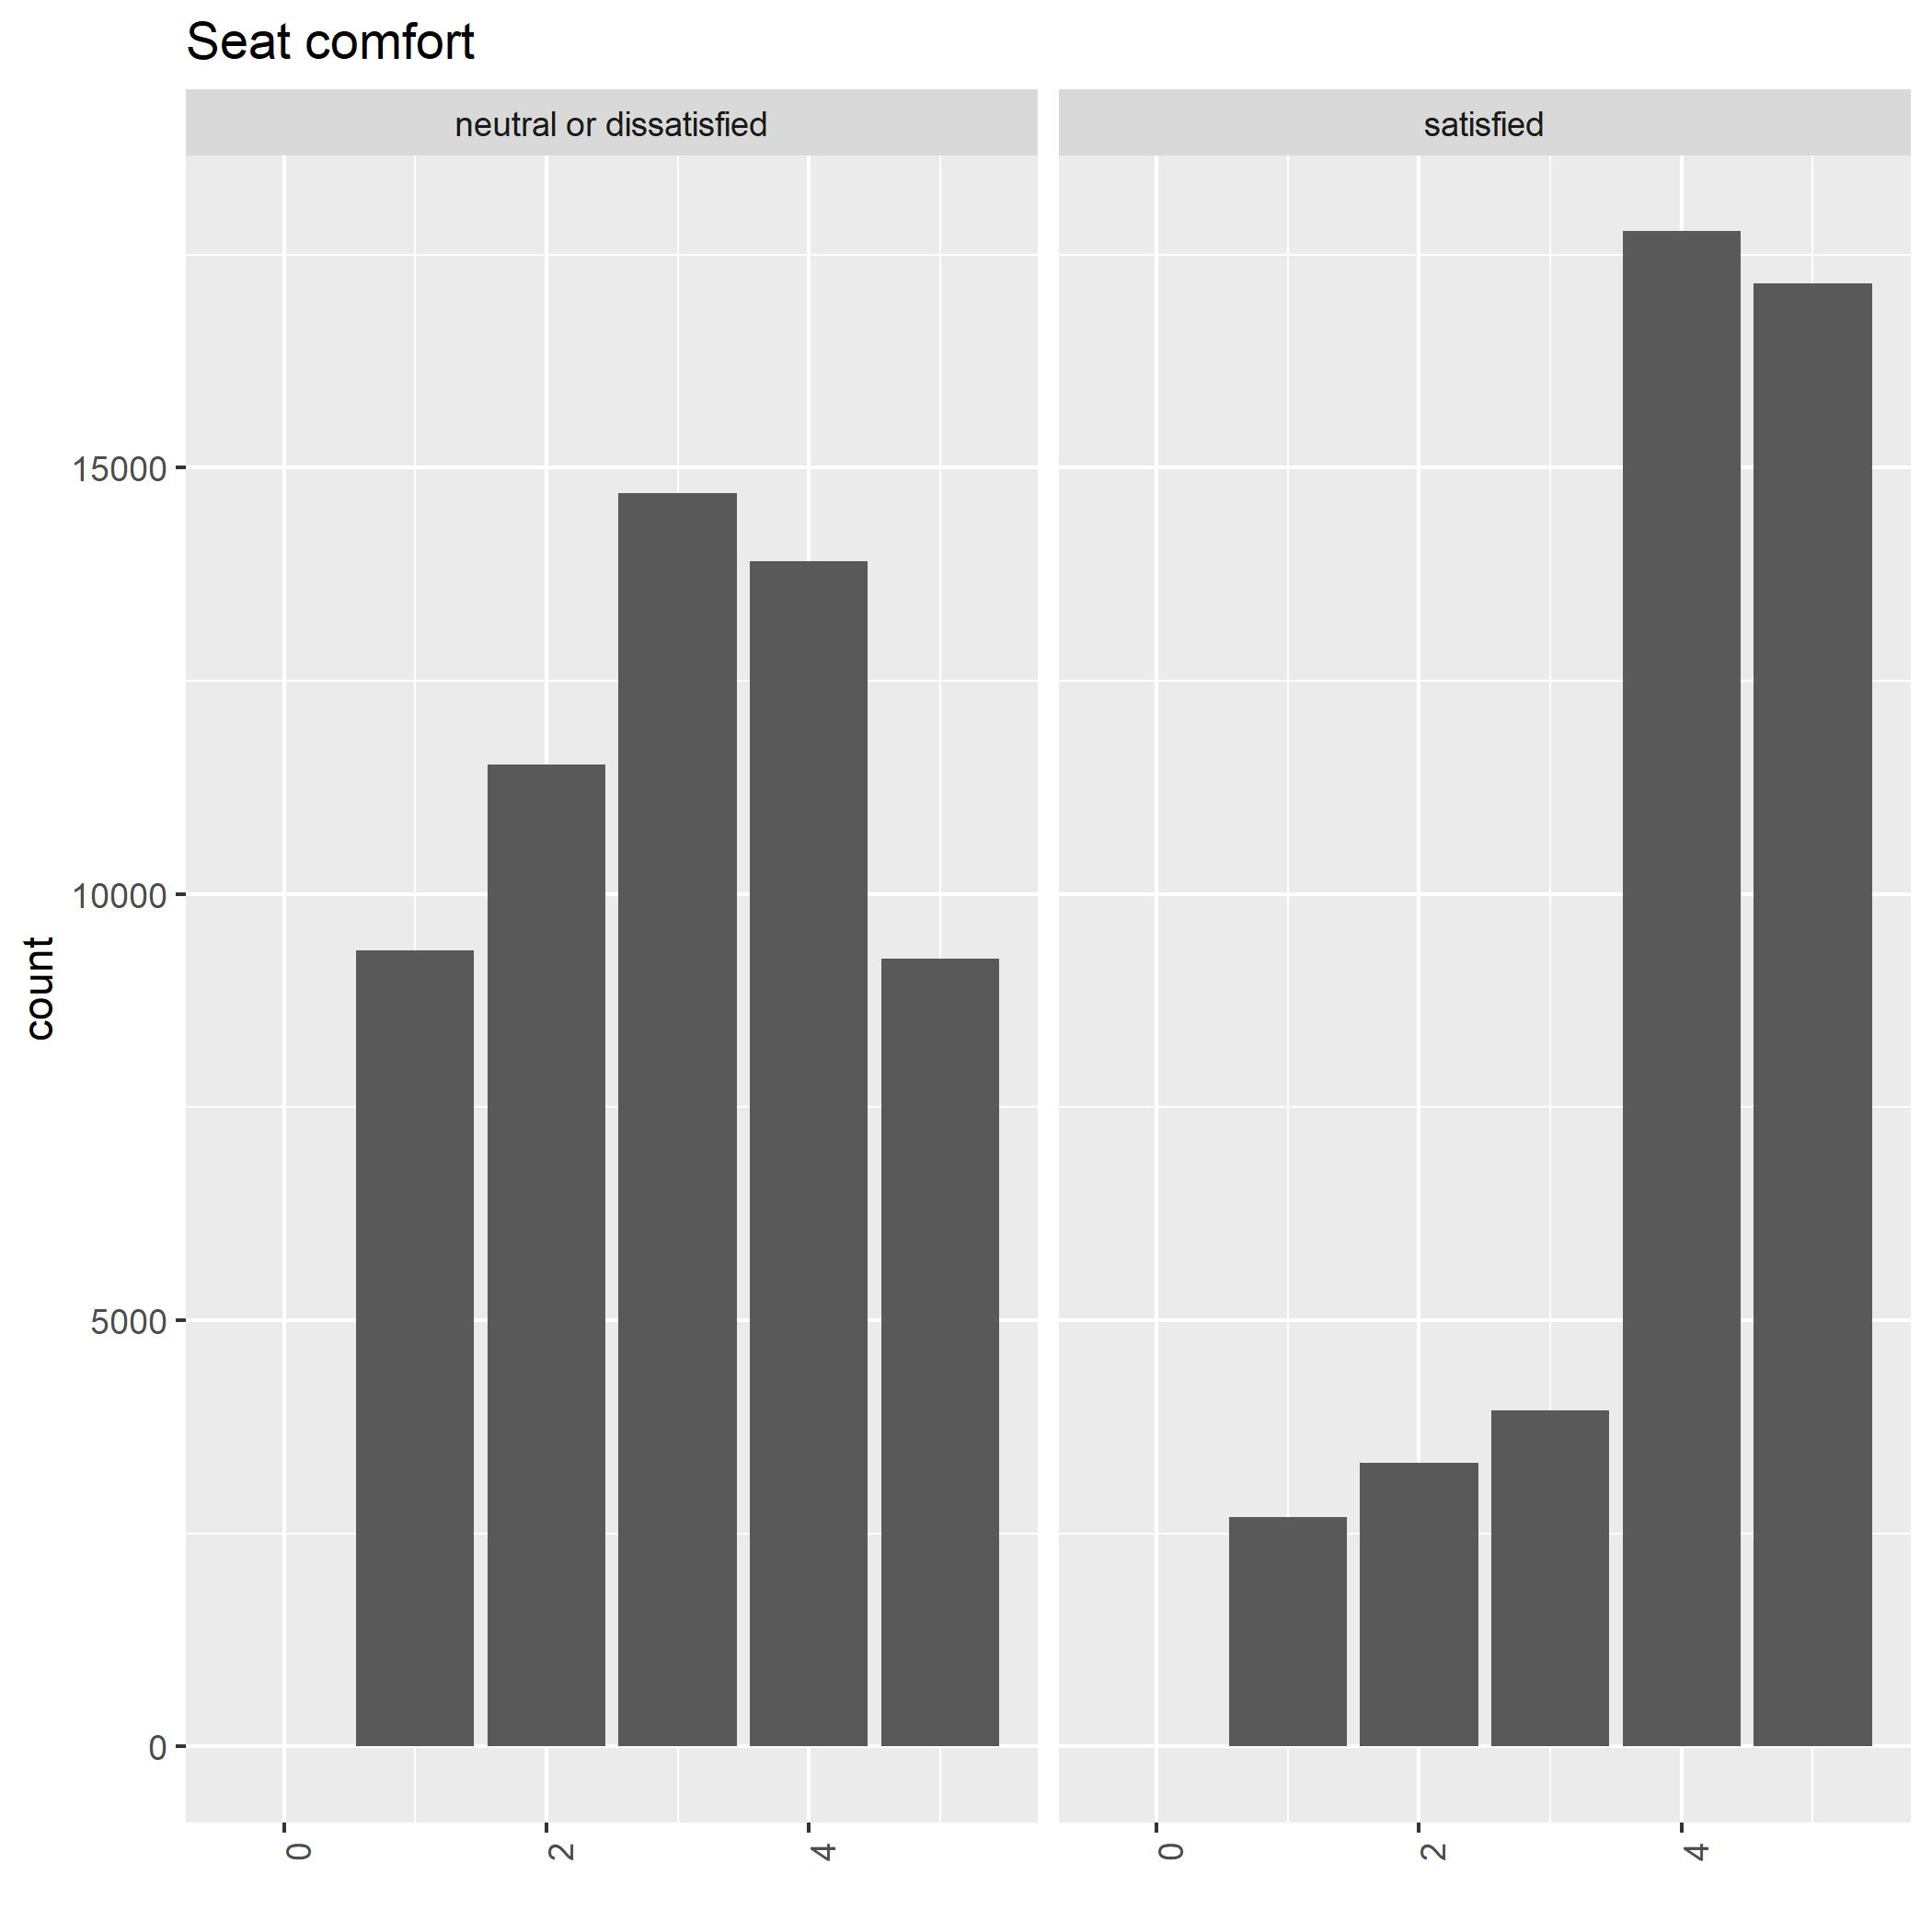
\includegraphics[width=.24\textwidth]{..//plots//plot13.jpg}\hfill
    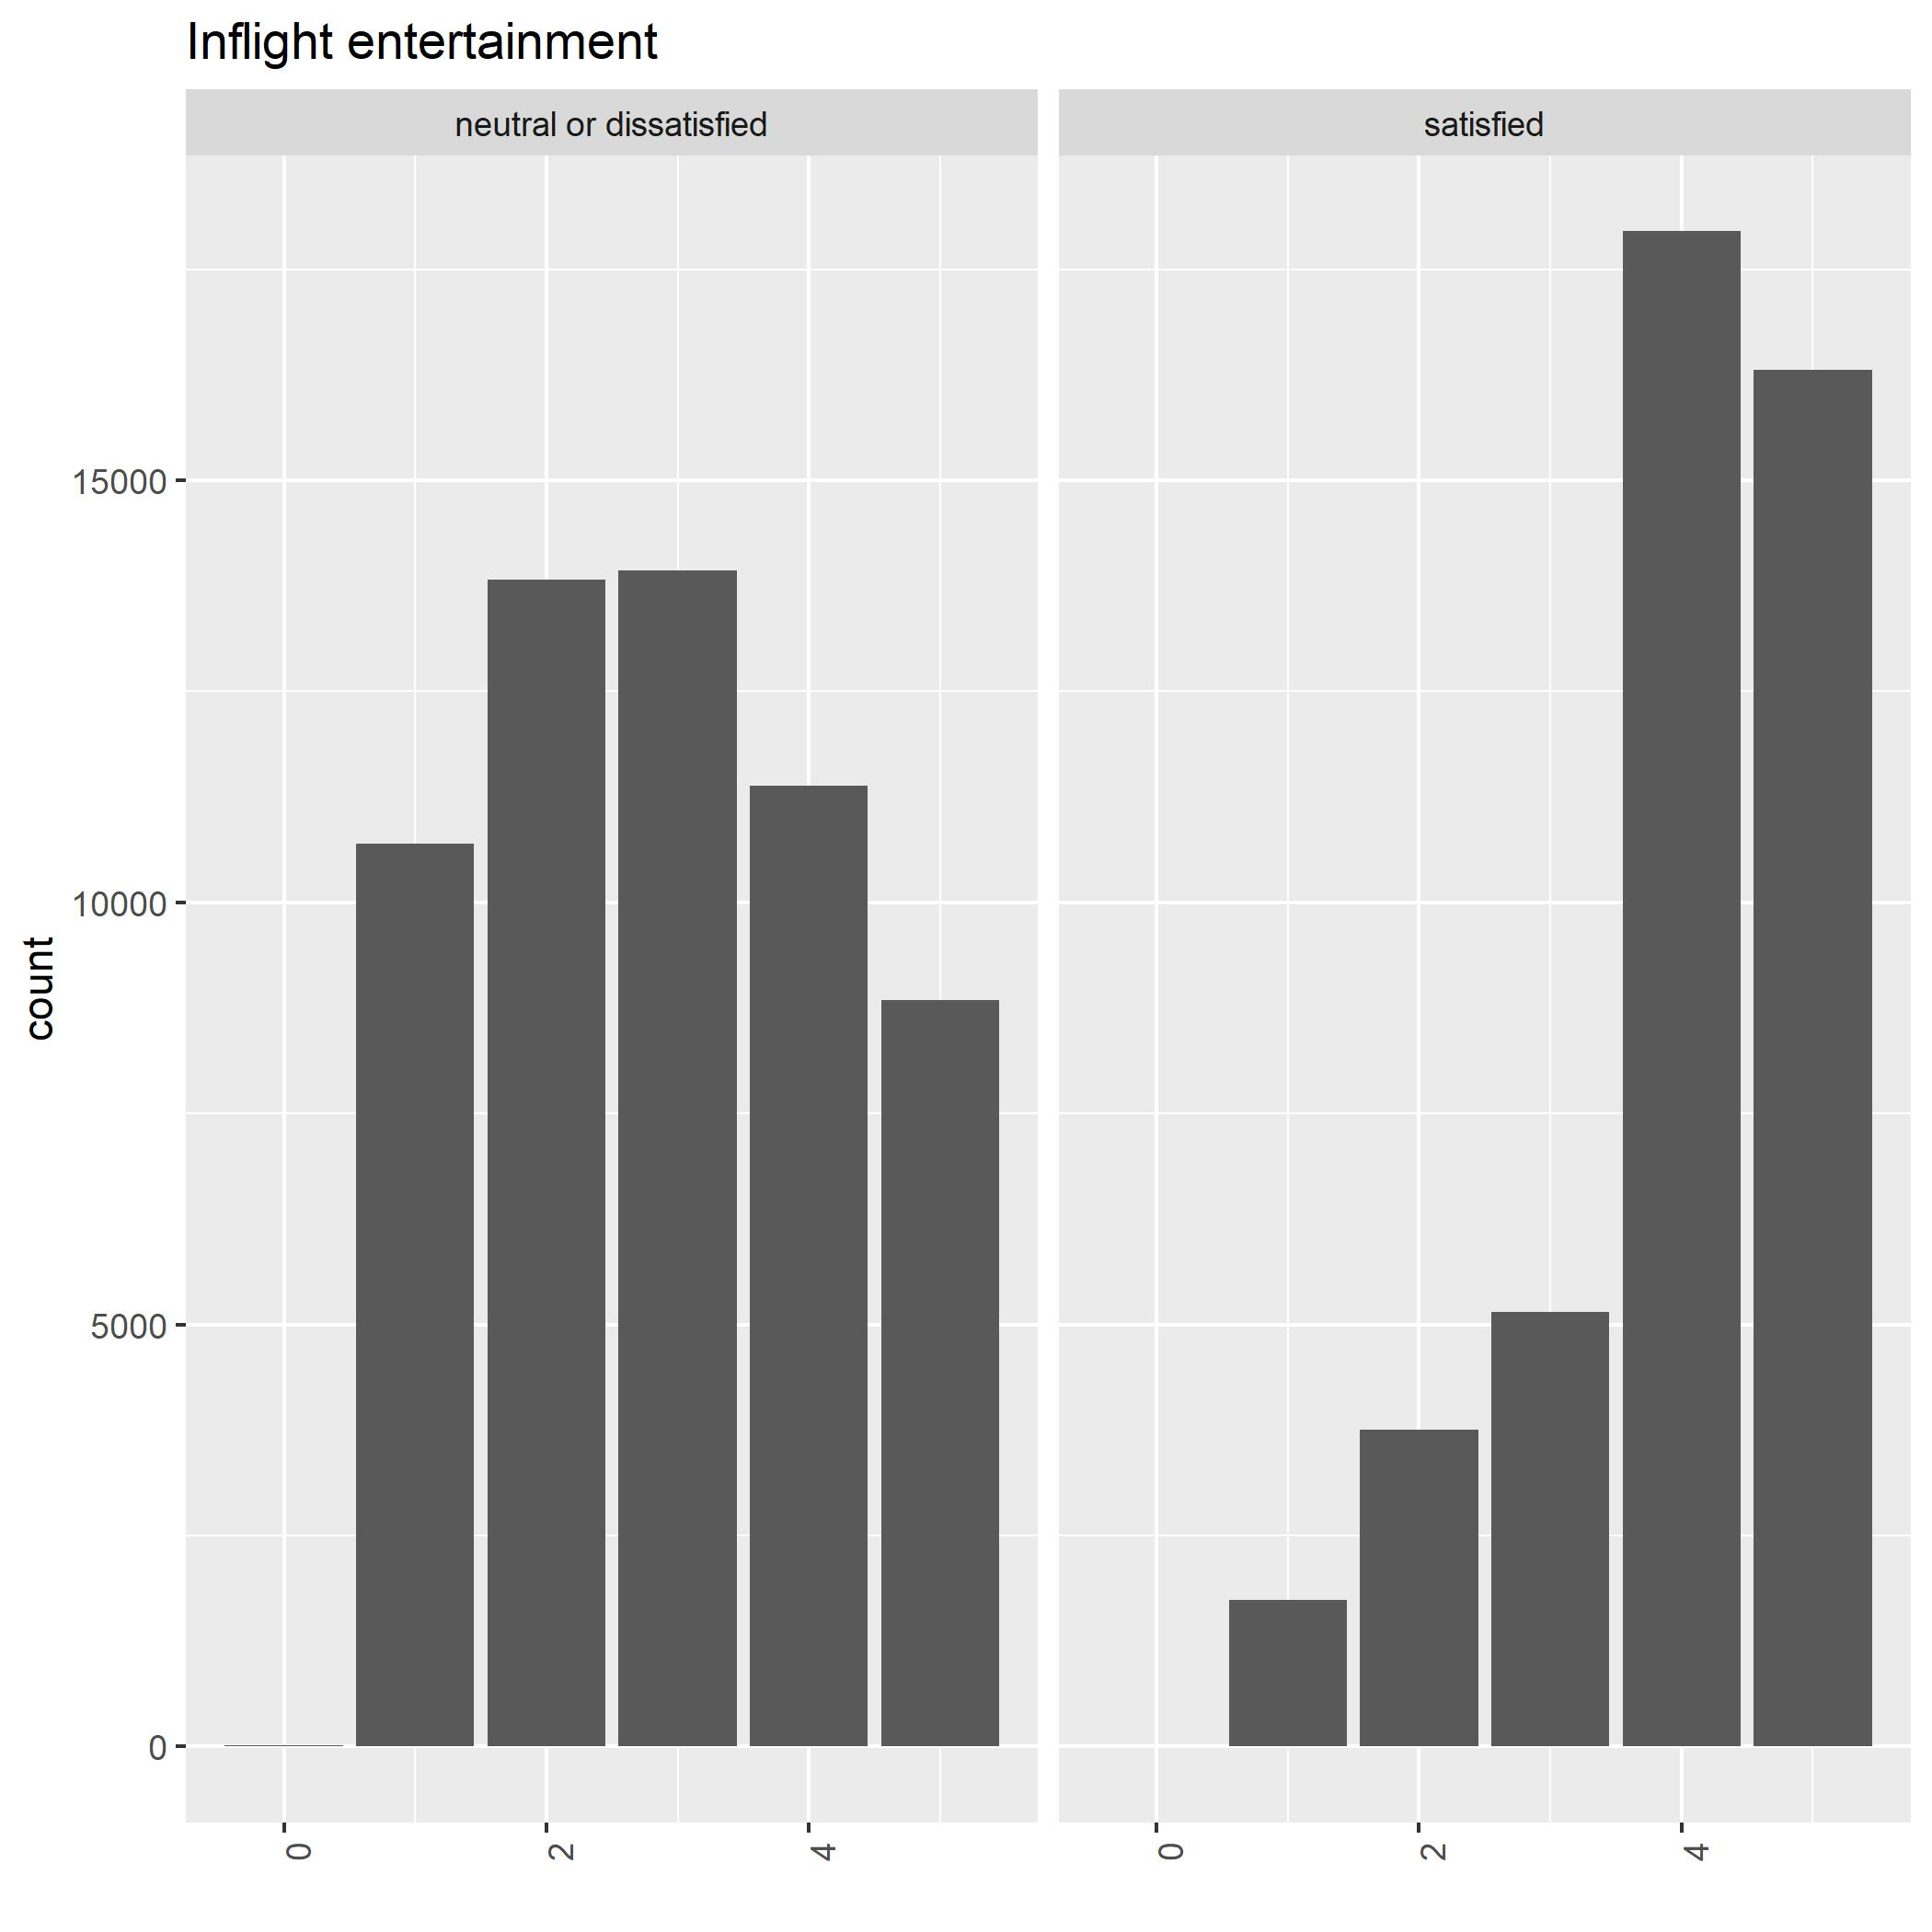
\includegraphics[width=.24\textwidth]{..//plots//plot14.jpg}\hfill
    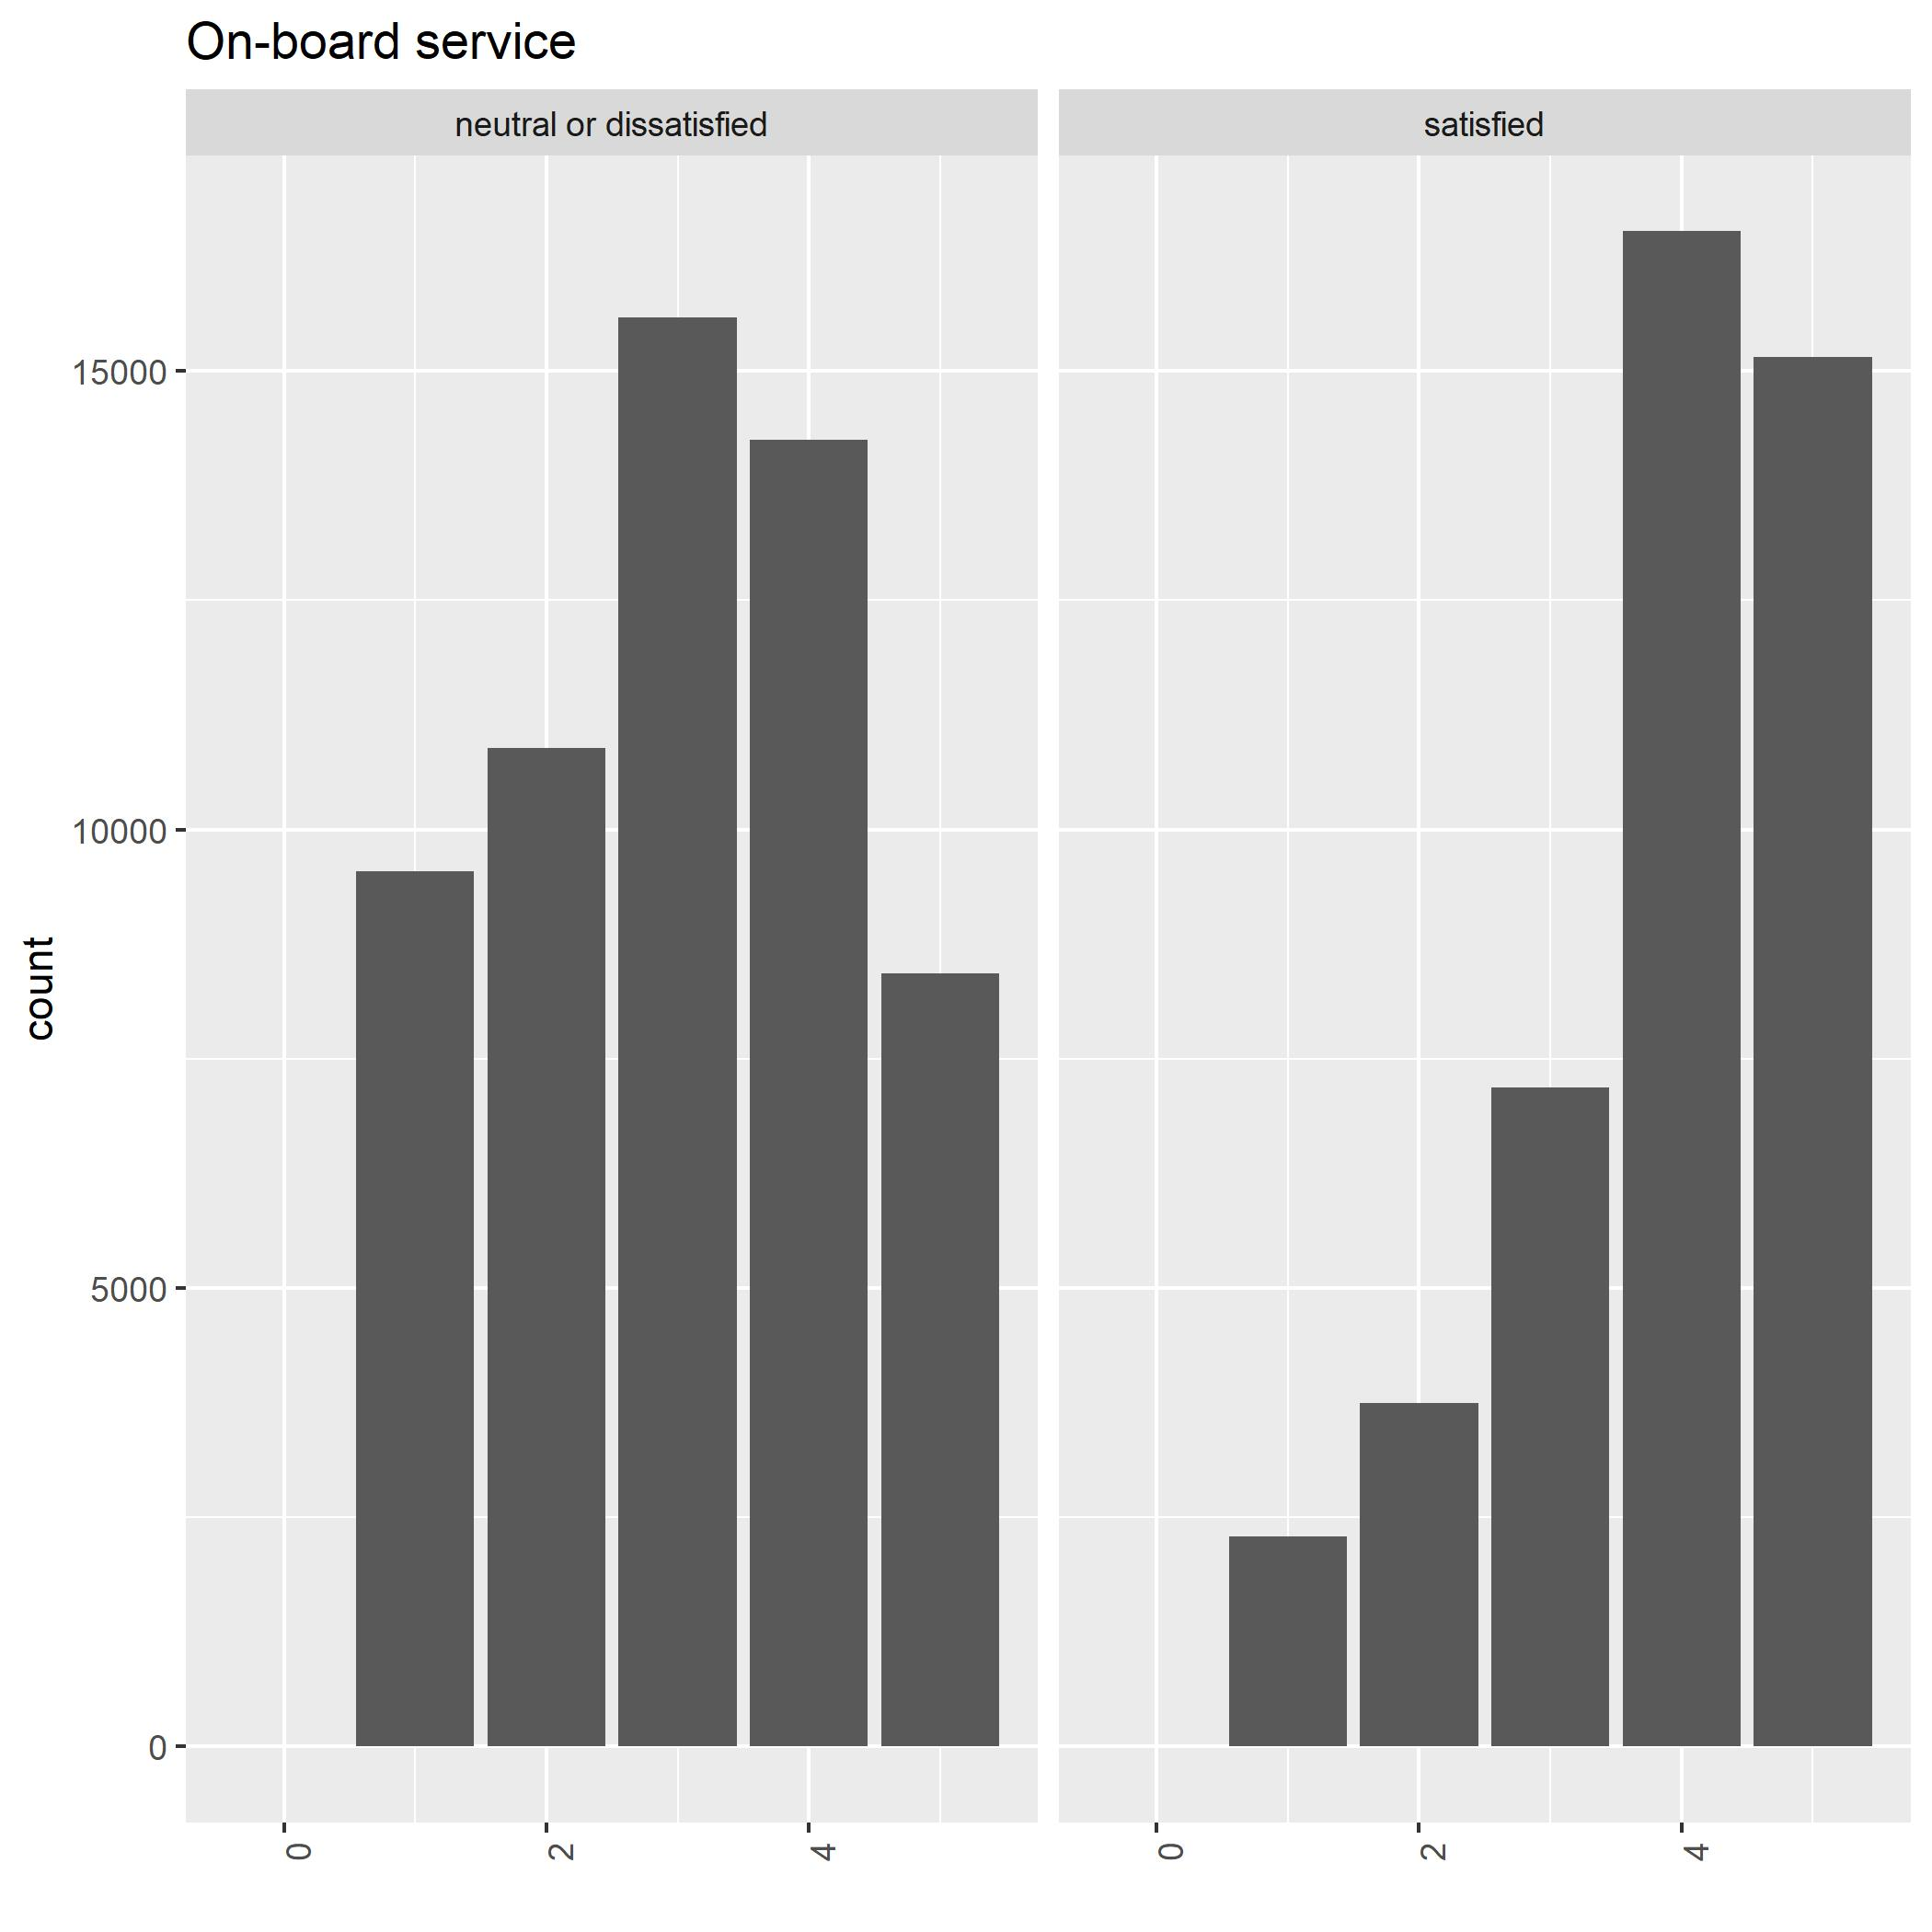
\includegraphics[width=.24\textwidth]{..//plots//plot15.jpg}\hfill
    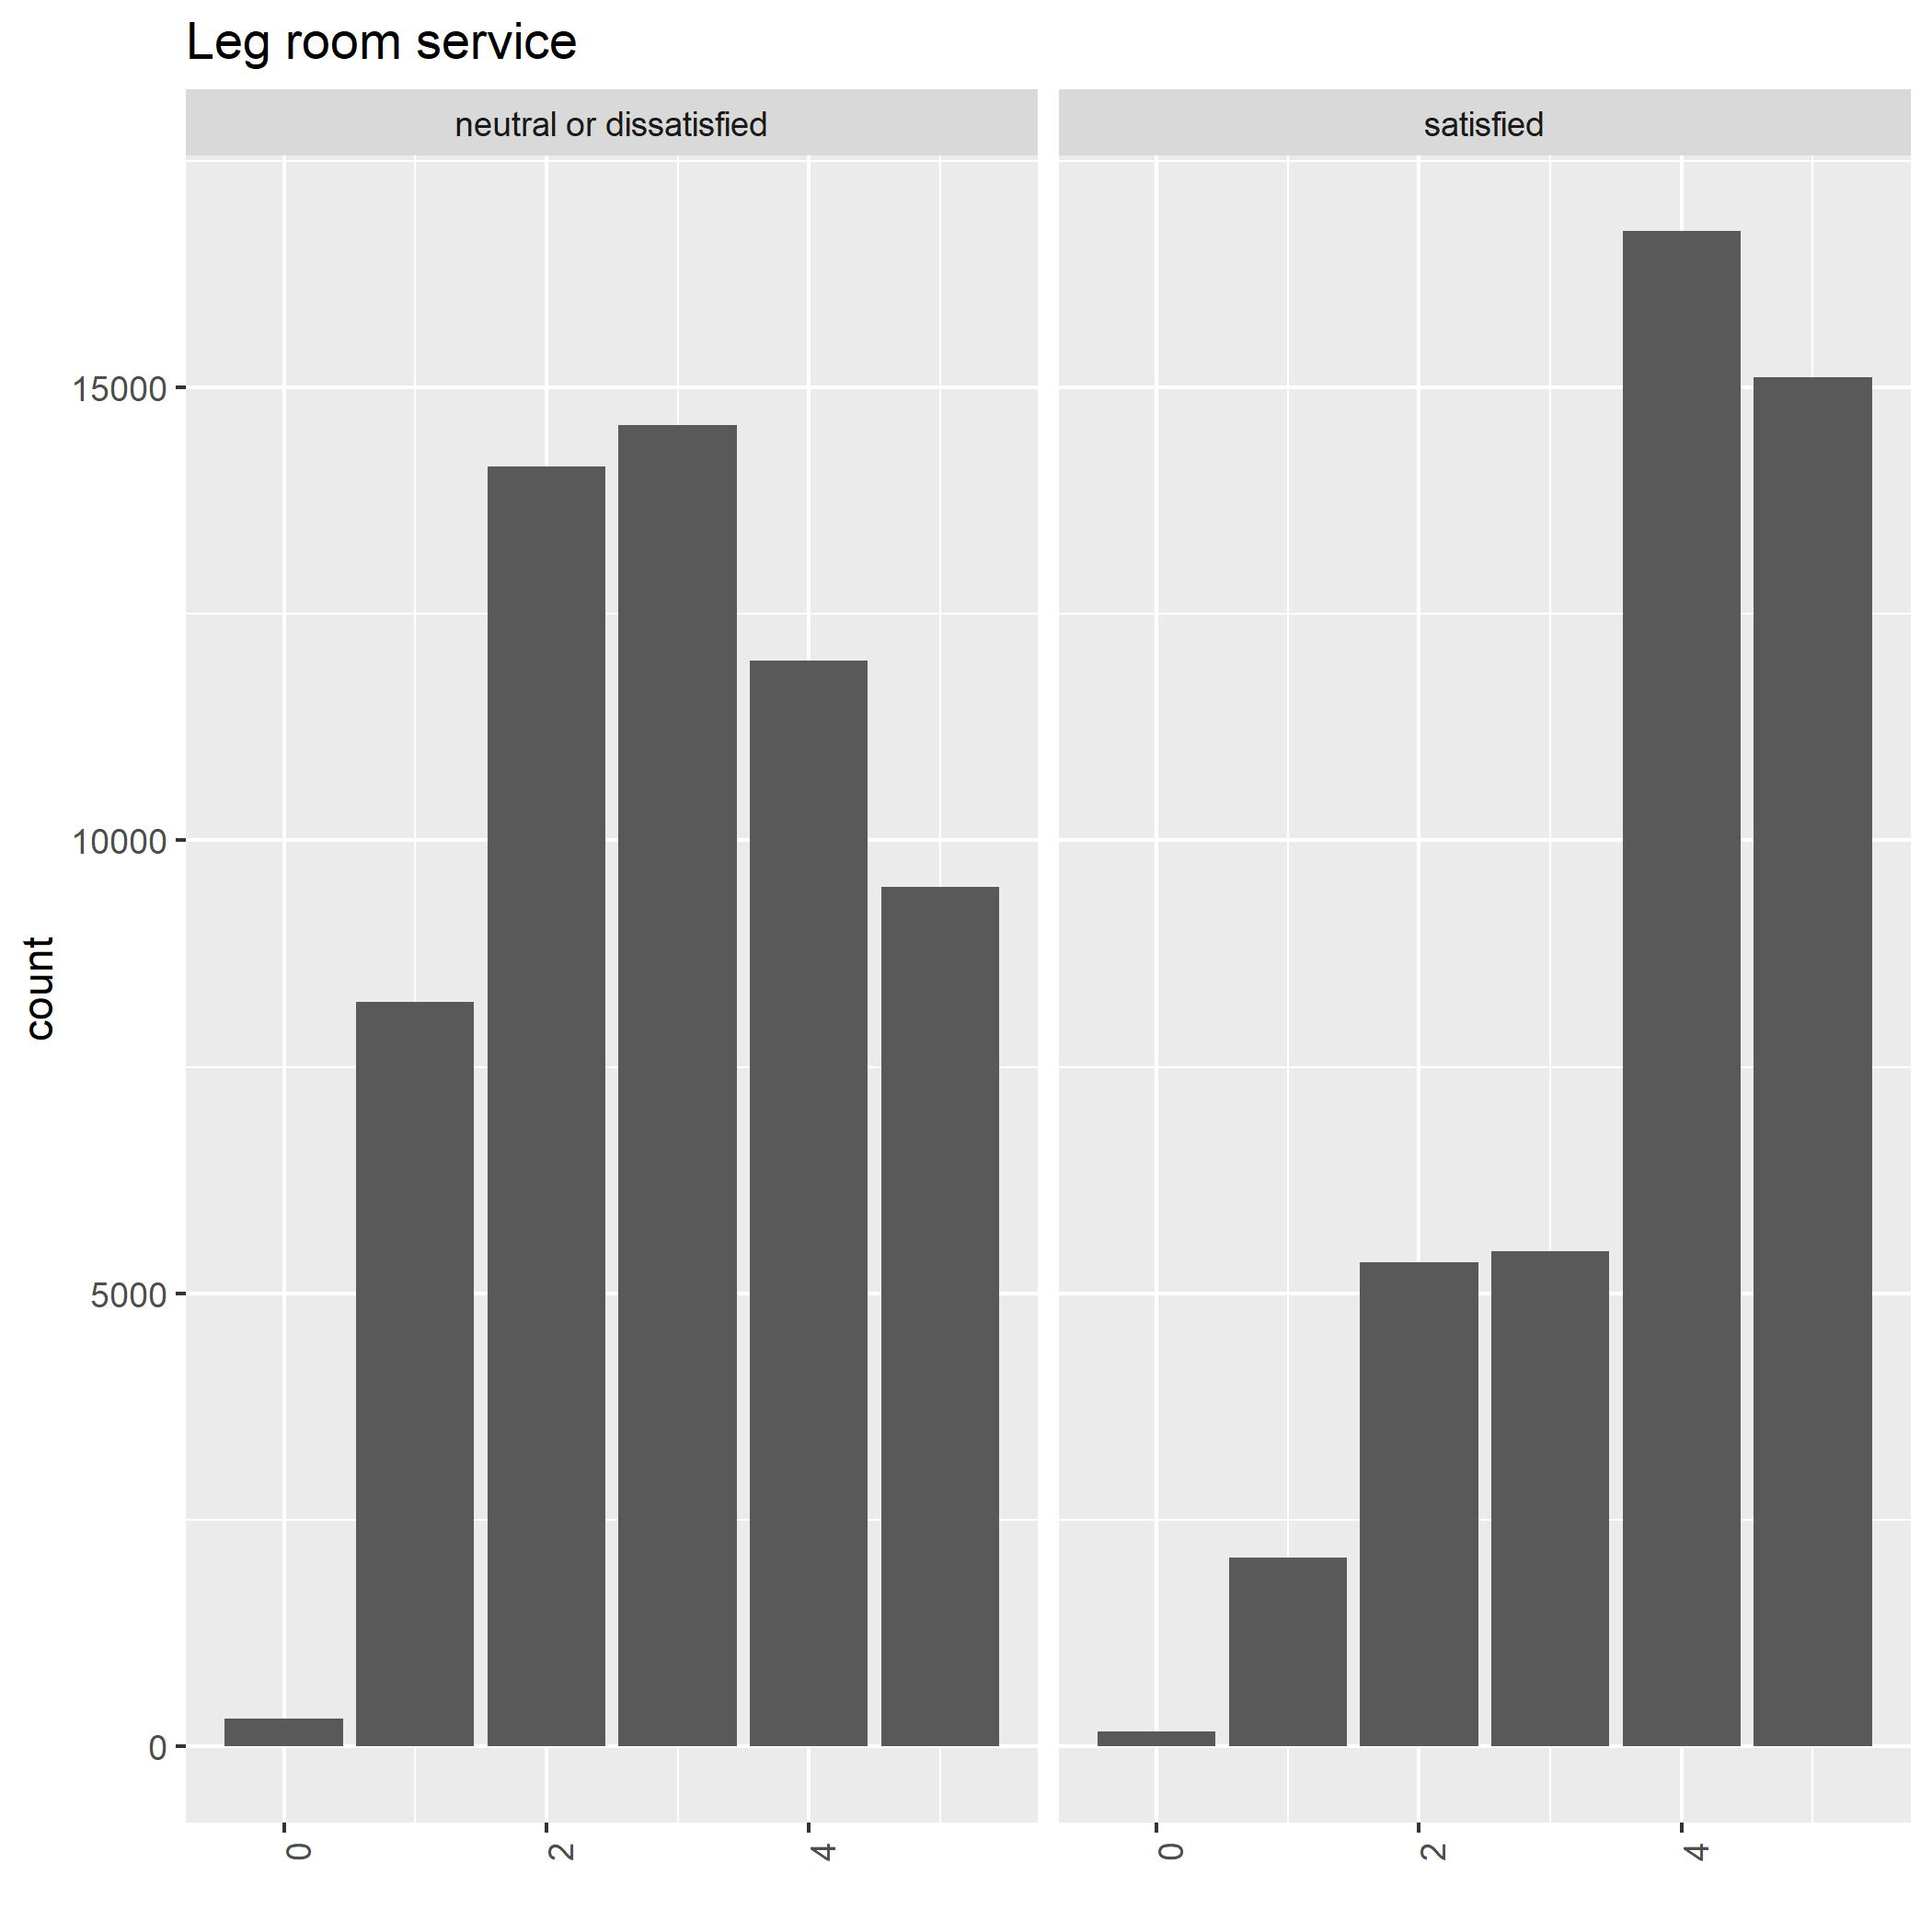
\includegraphics[width=.24\textwidth]{..//plots//plot16.jpg}\hfill
    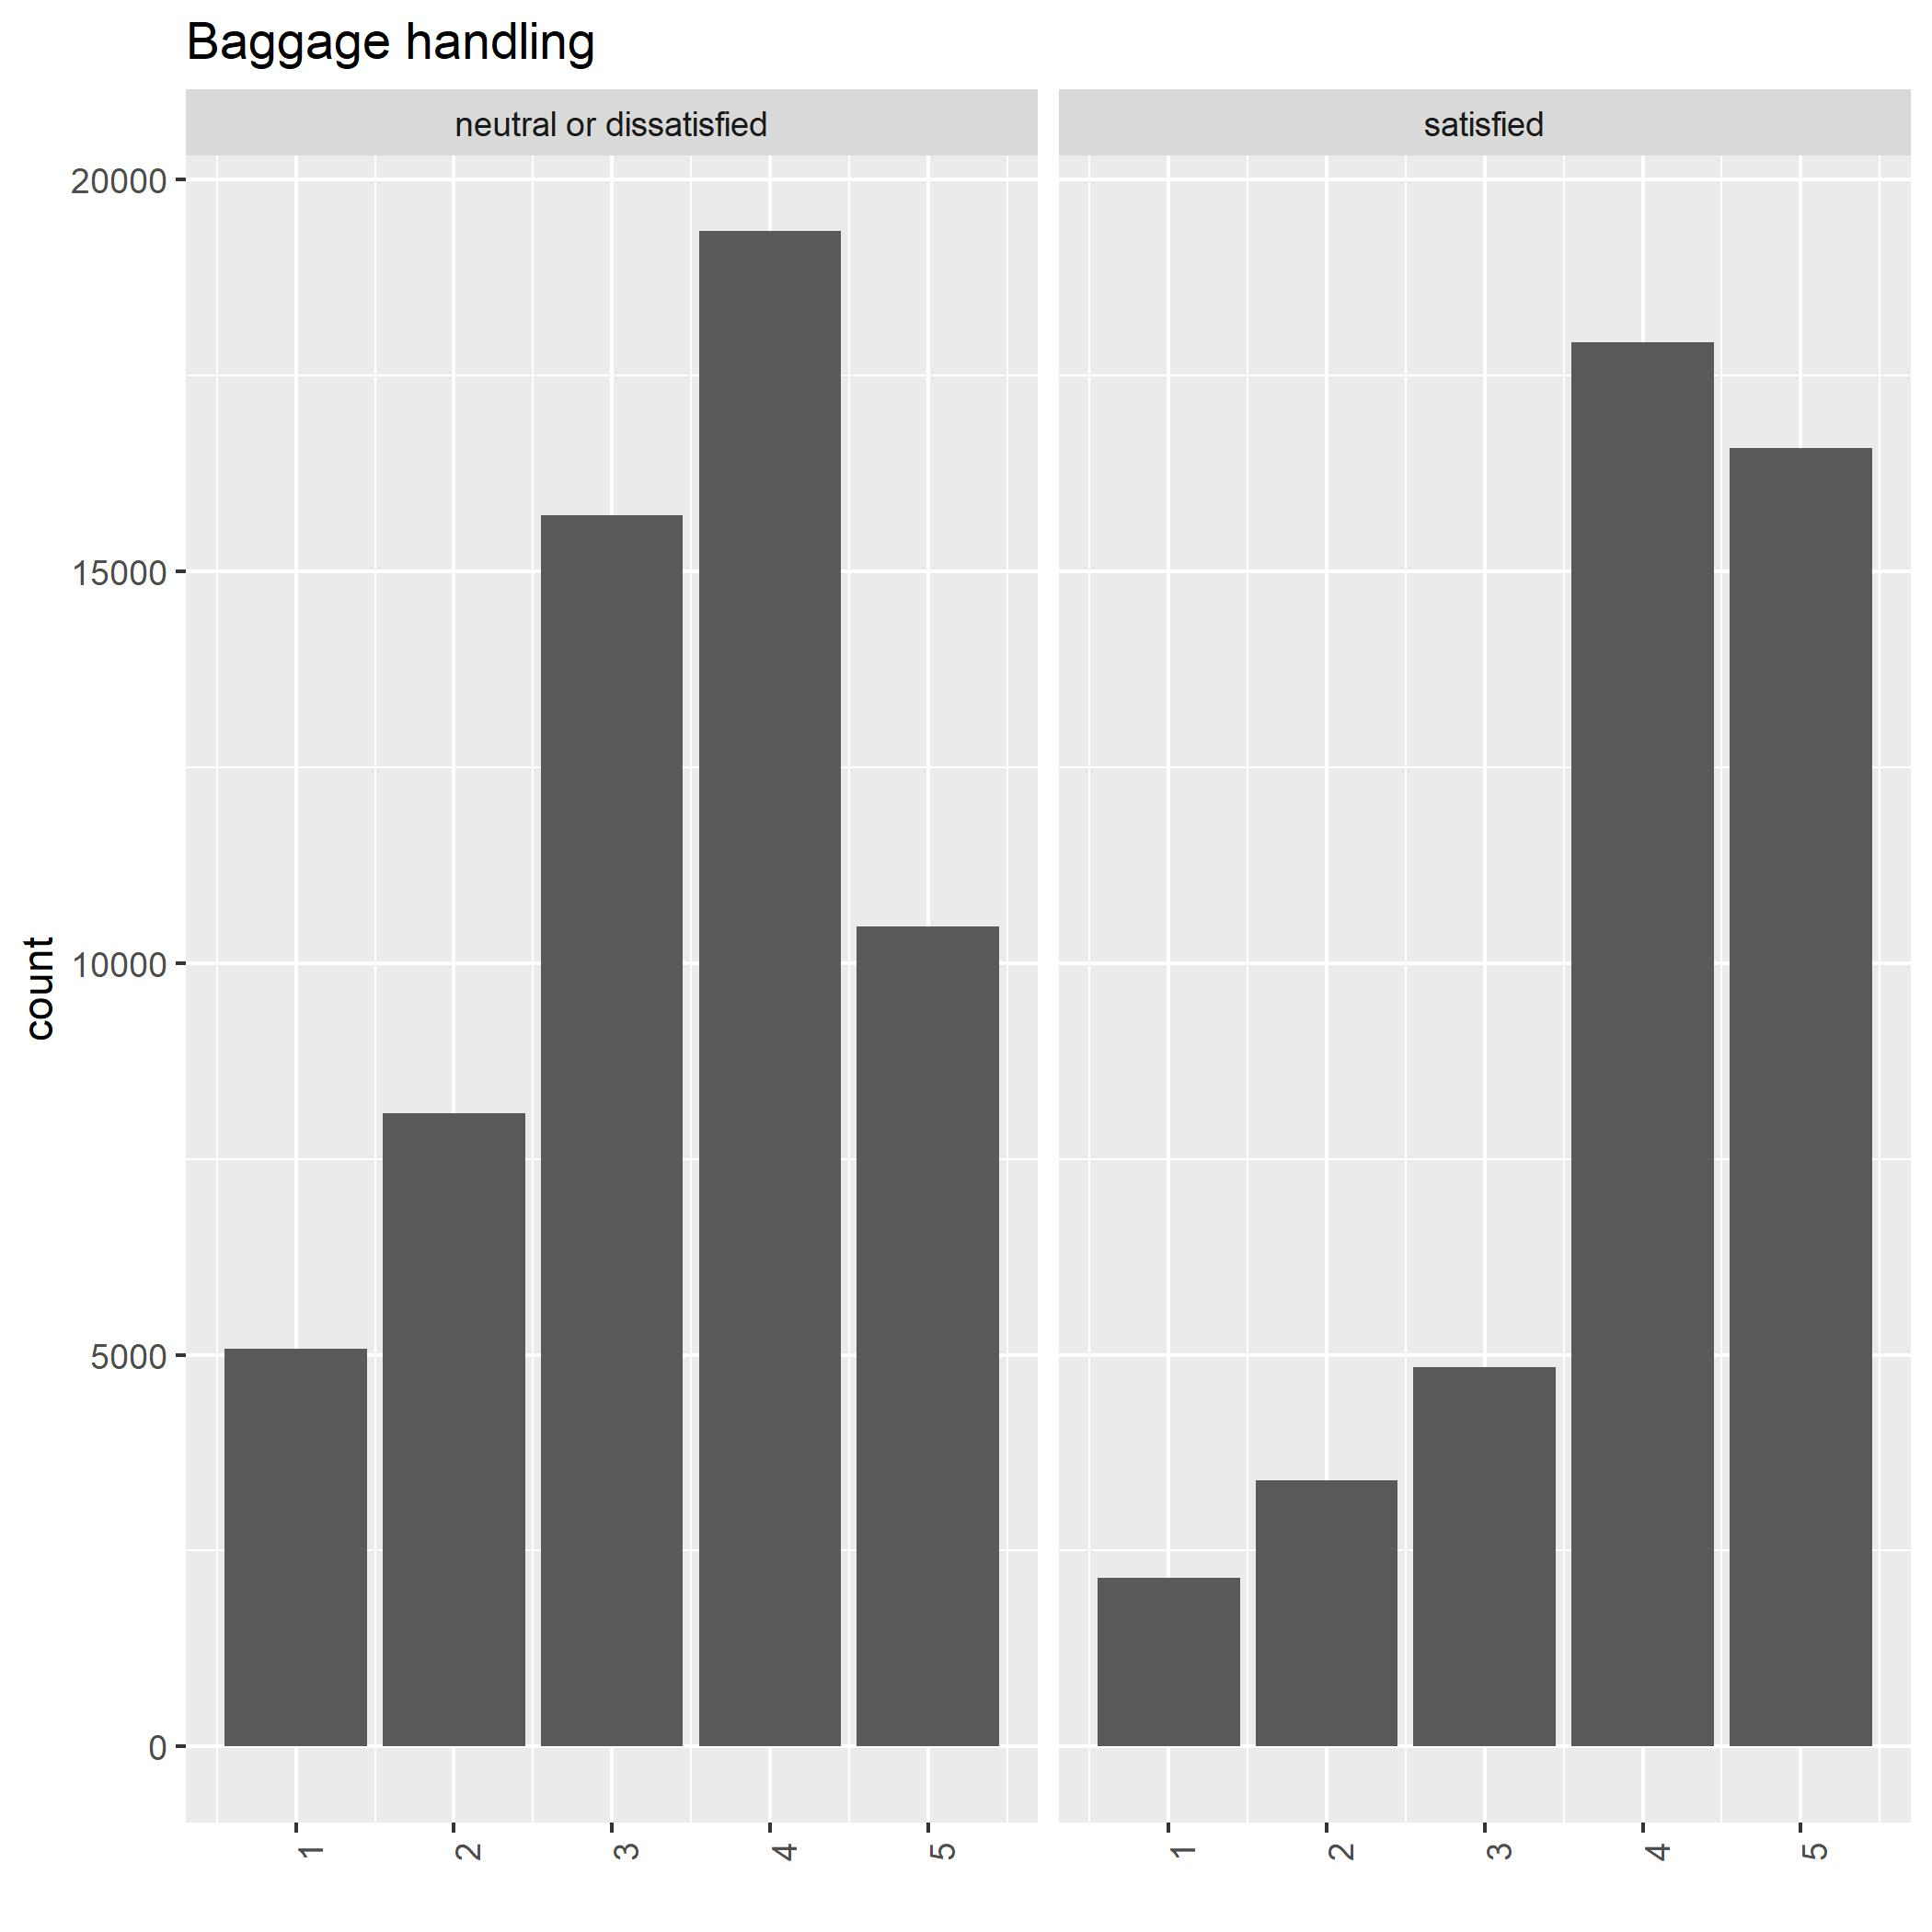
\includegraphics[width=.24\textwidth]{..//plots//plot17.jpg}\hfill
    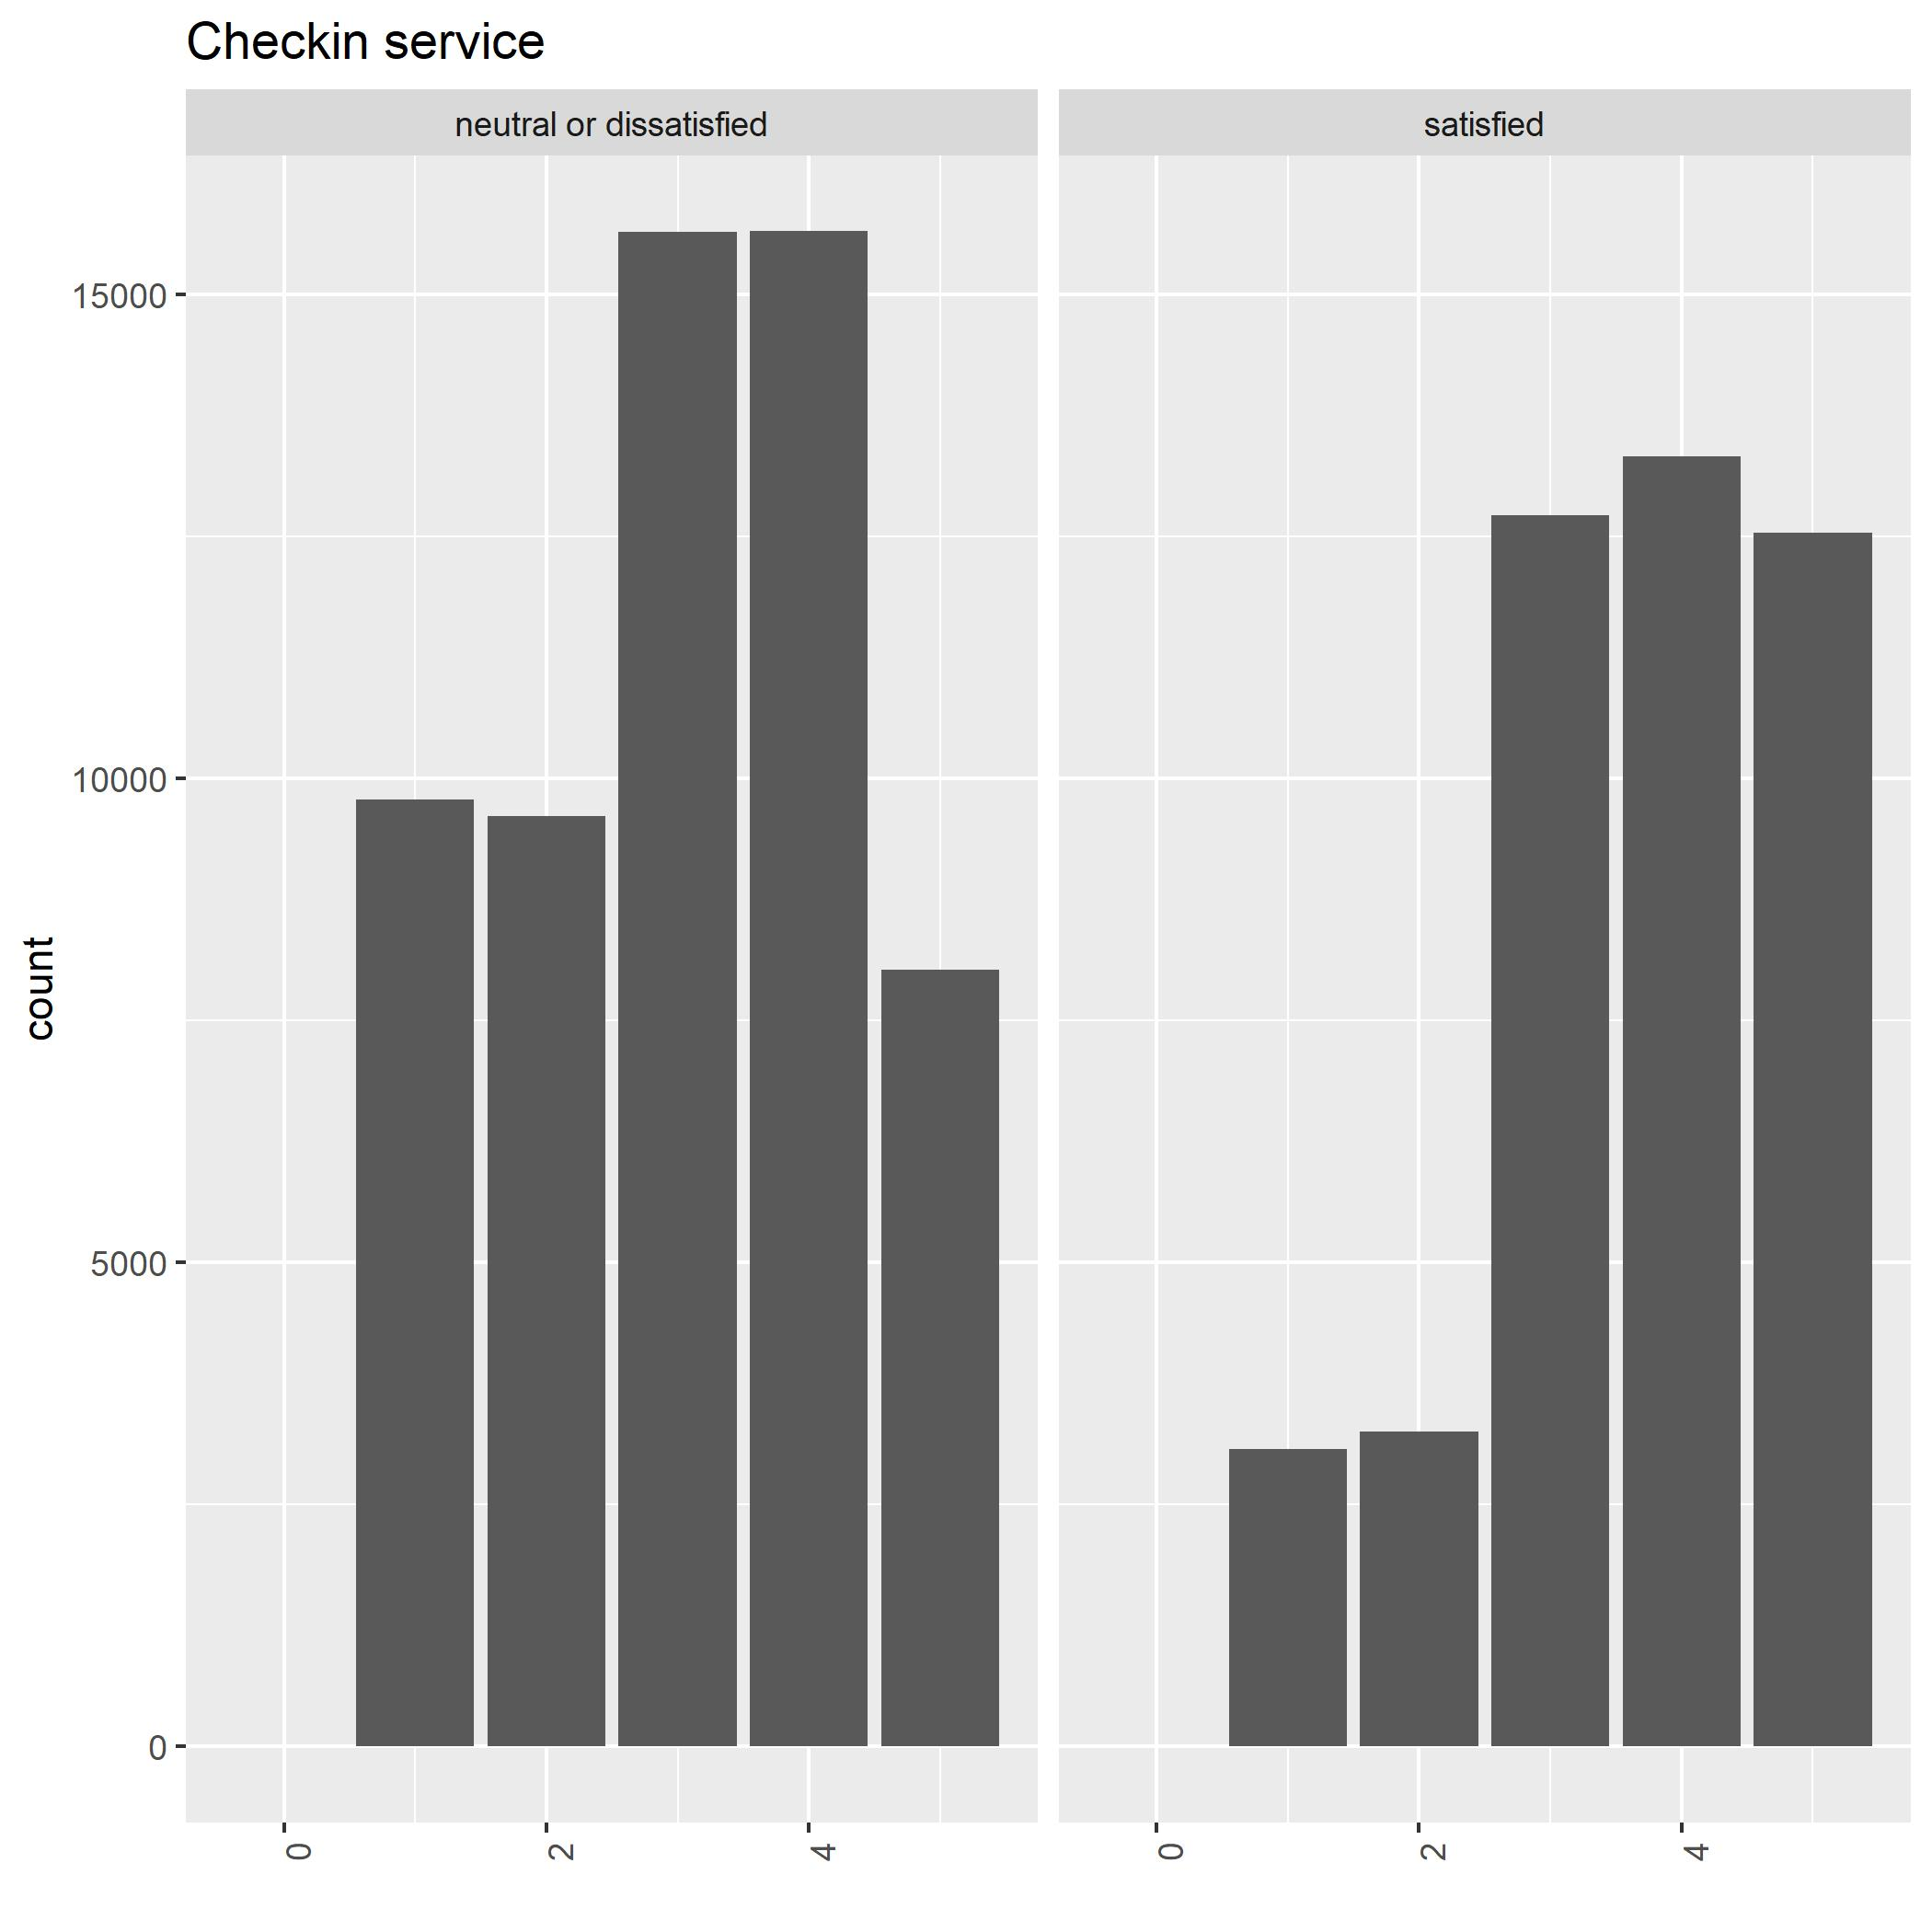
\includegraphics[width=.24\textwidth]{..//plots//plot18.jpg}\hfill
    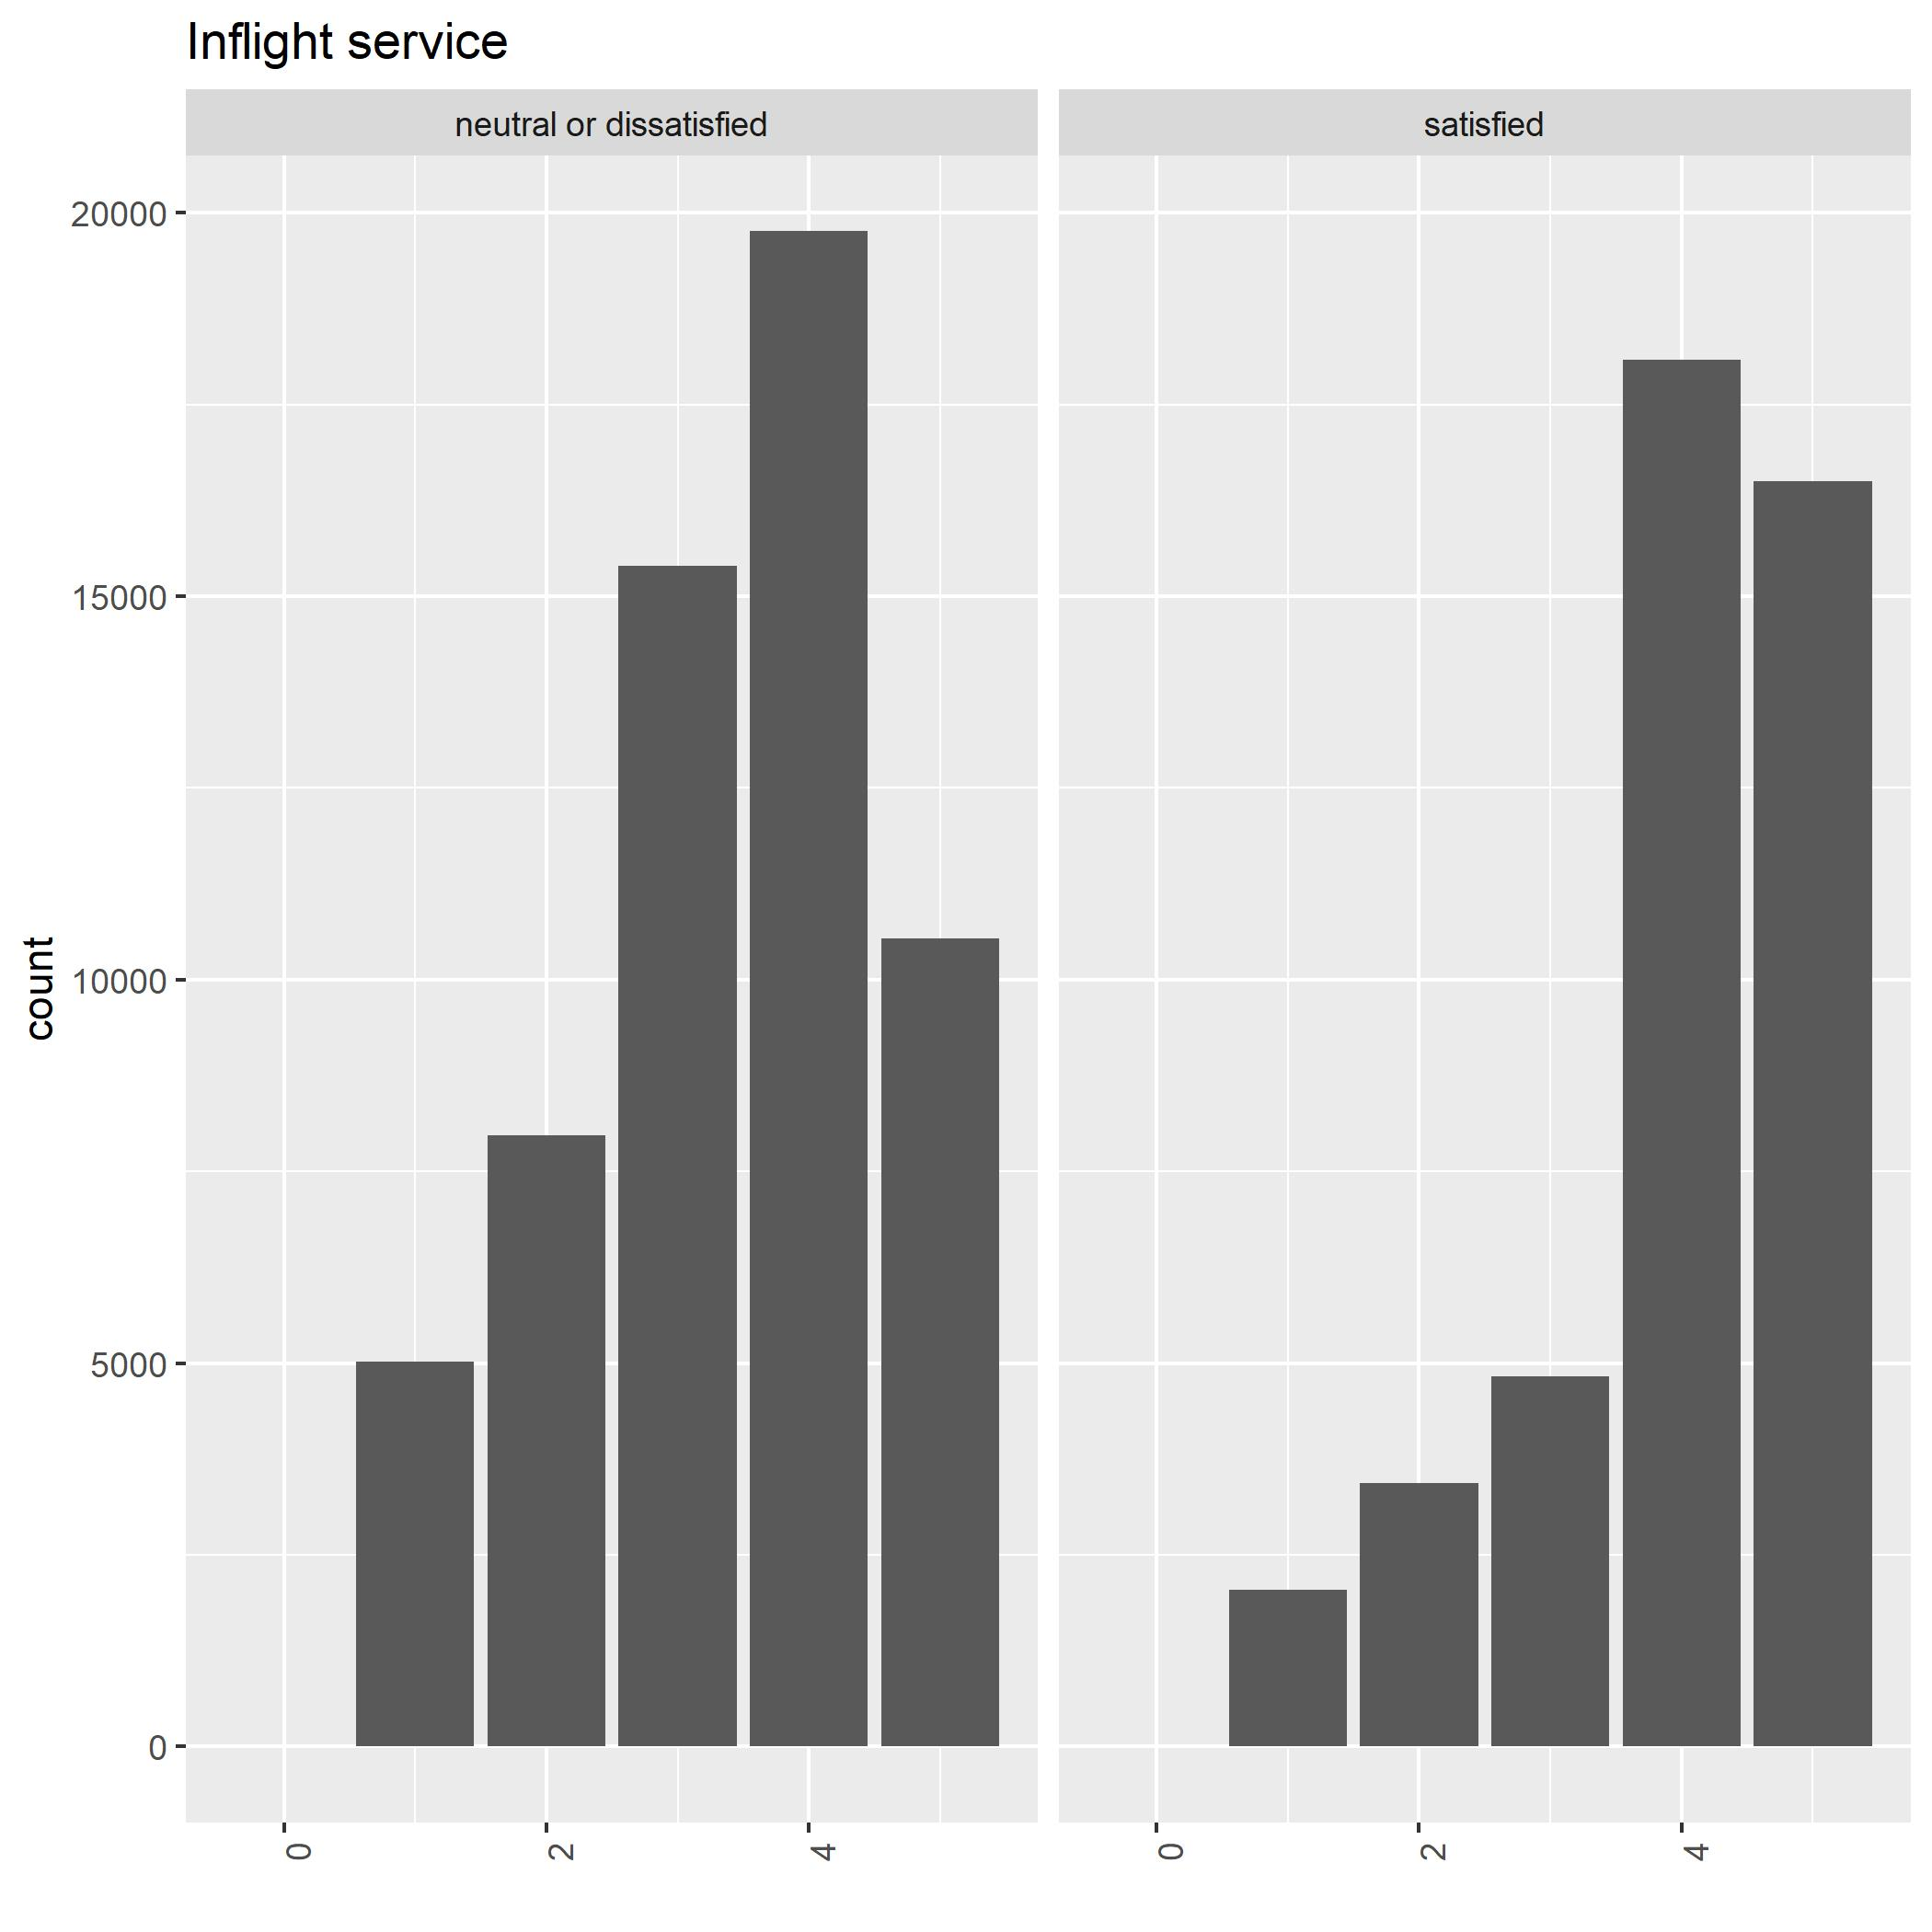
\includegraphics[width=.24\textwidth]{..//plots//plot19.jpg}\hfill
    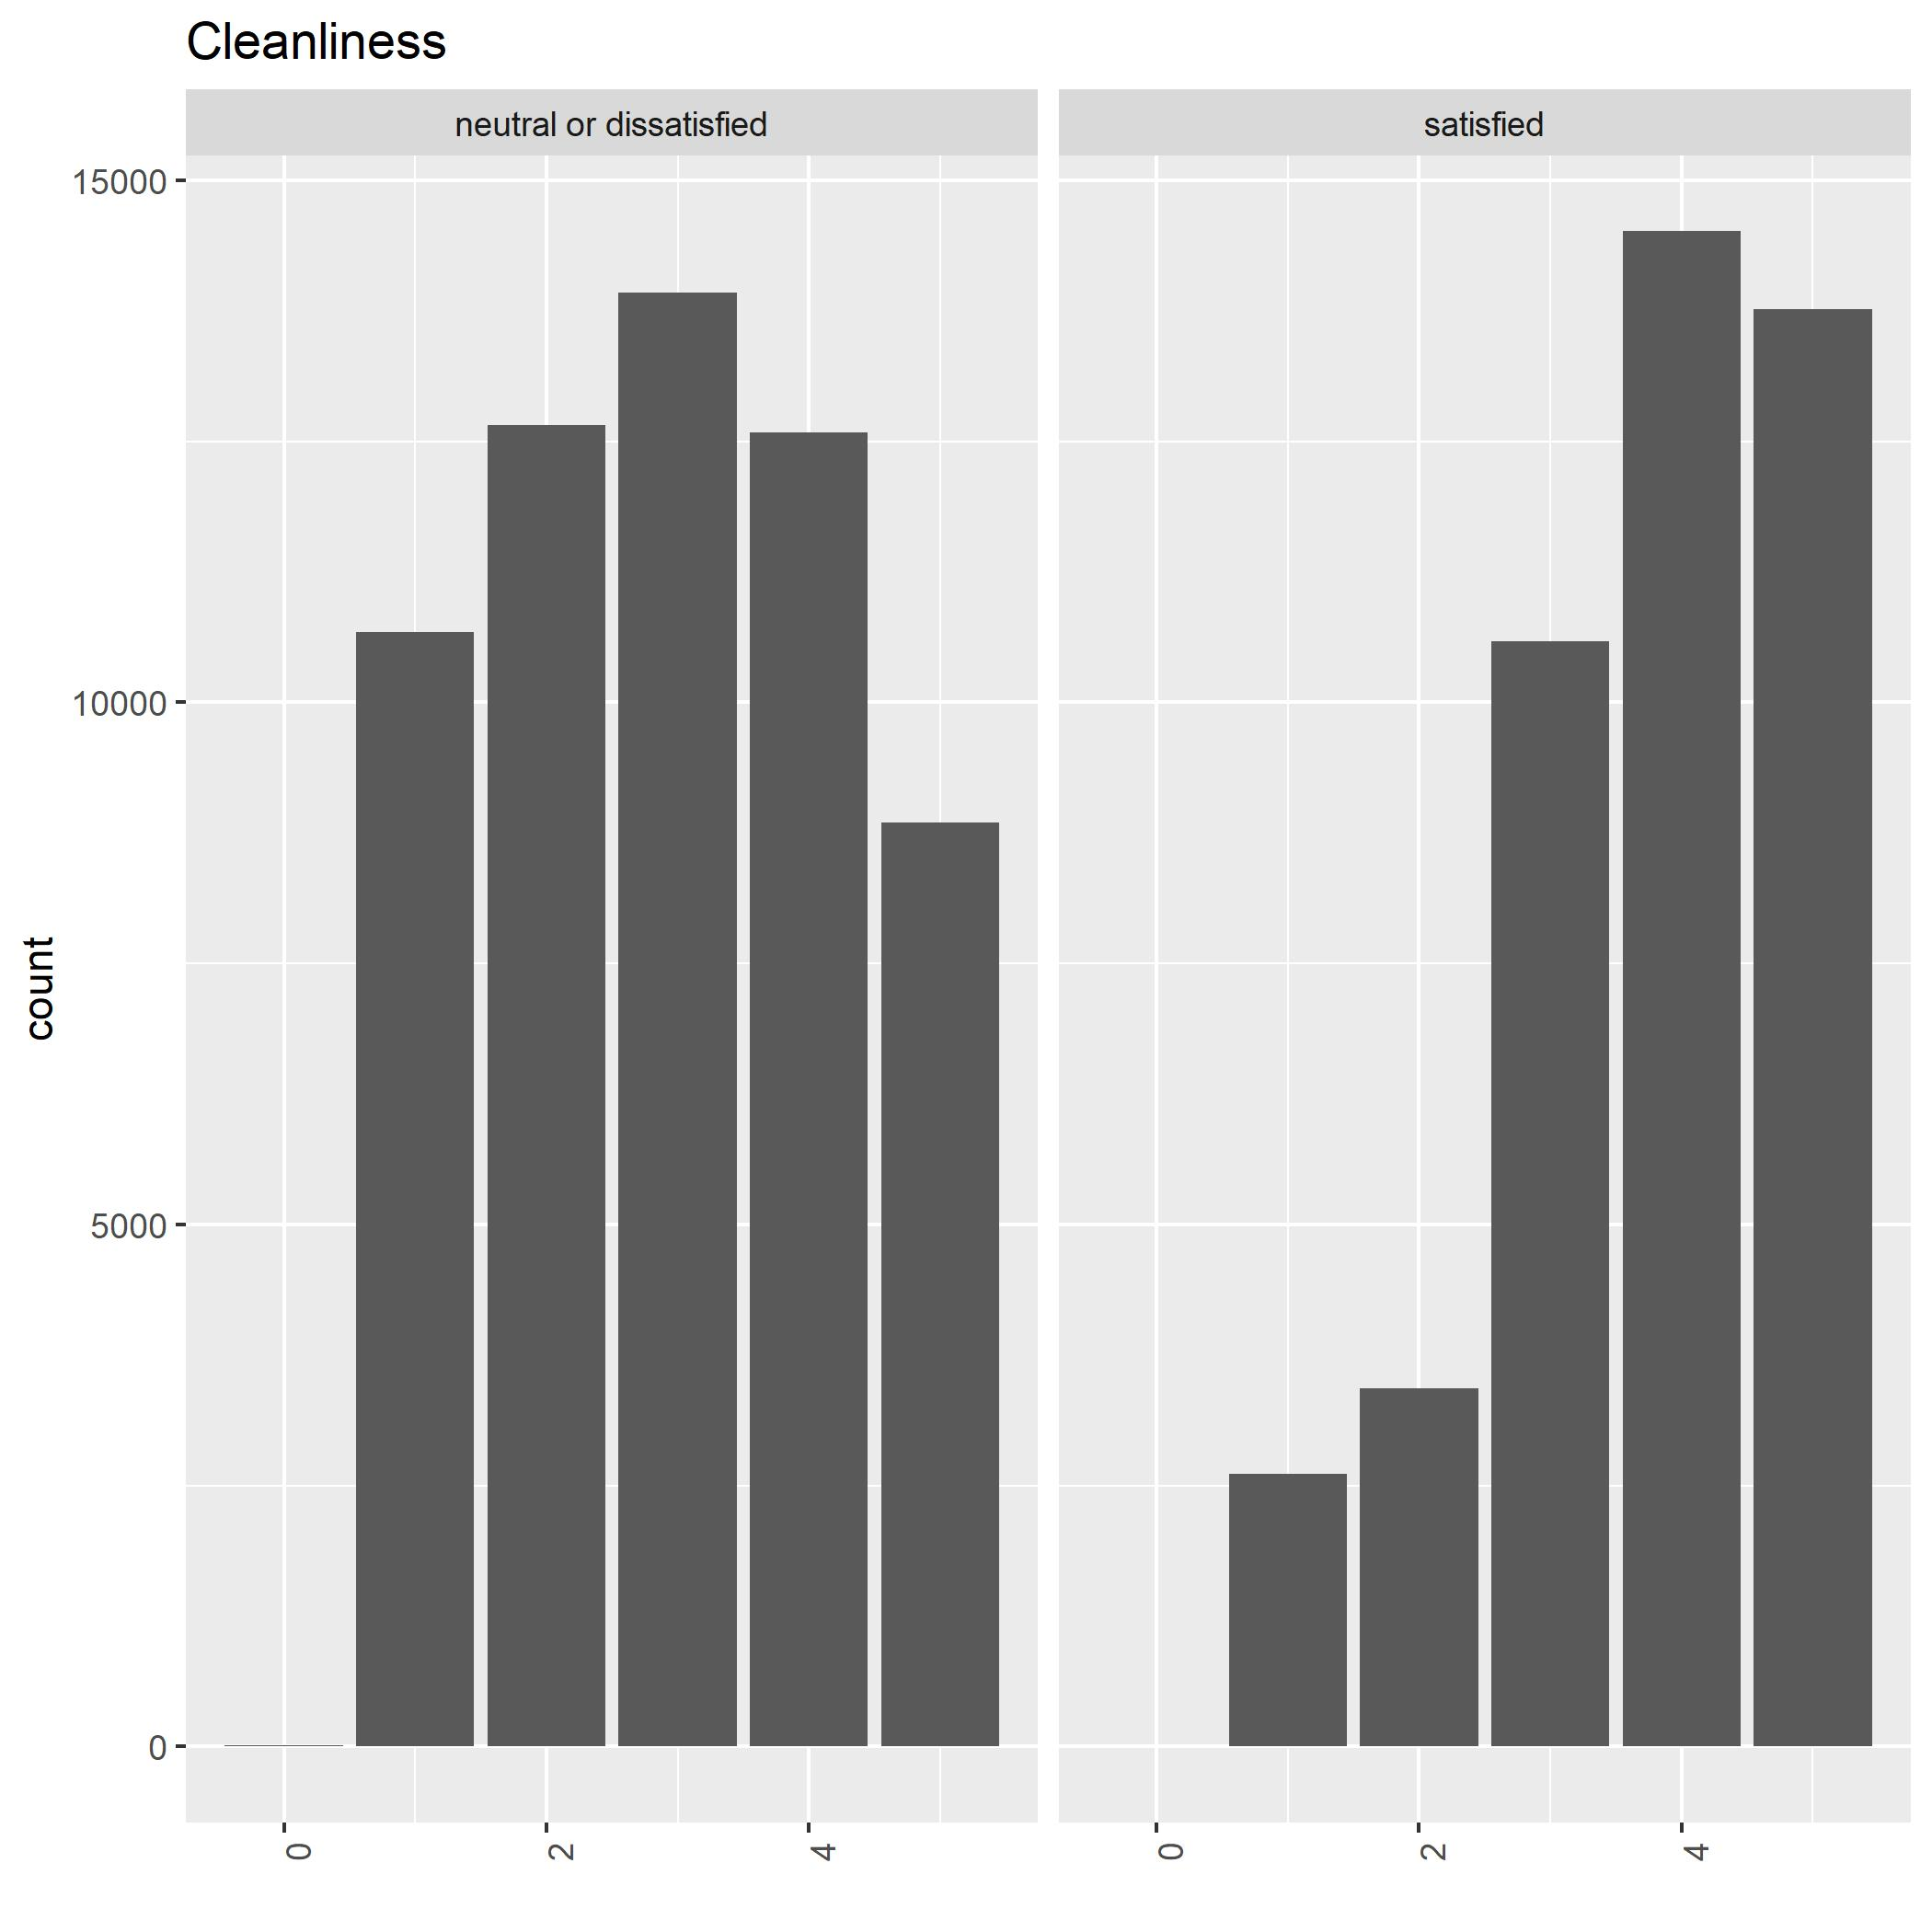
\includegraphics[width=.24\textwidth]{..//plots//plot20.jpg}\hfill
    \caption{Vizualisation of all ordinal variables by criterion}\label{fig:foobar}
\end{figure}

\begin{figure}
    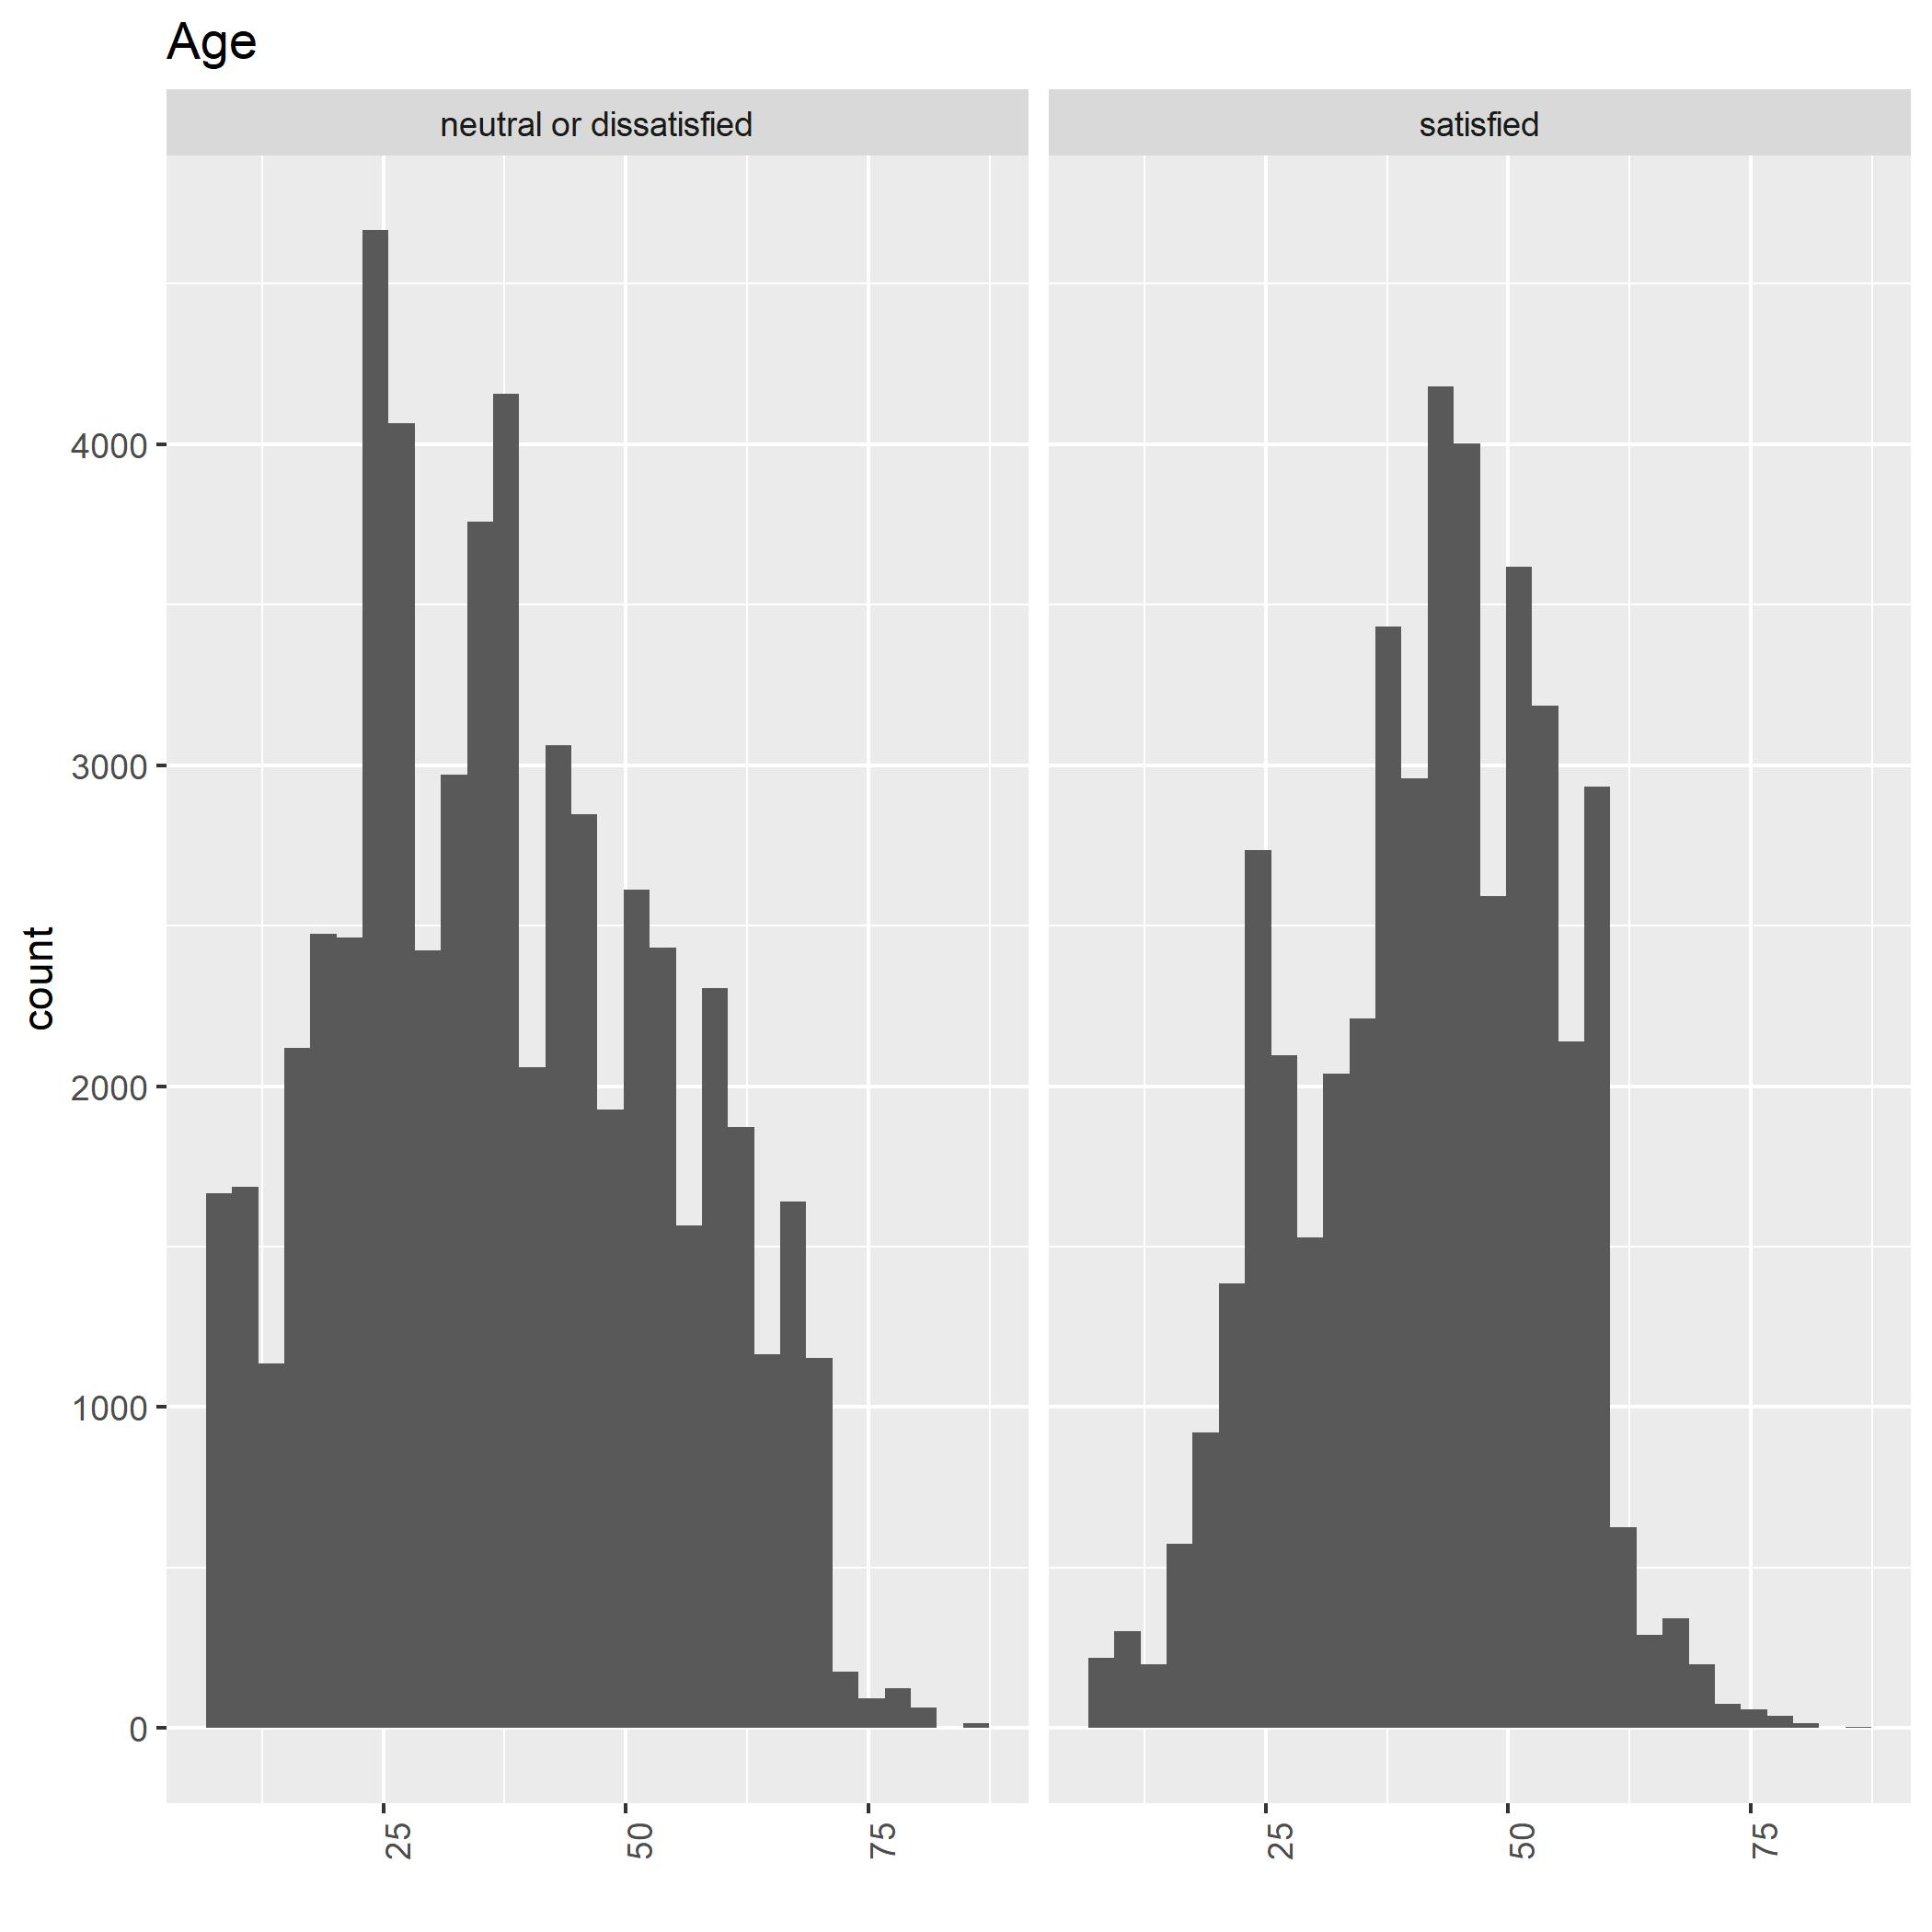
\includegraphics[width=.24\textwidth]{..//plots//plot3.jpg}\hfill
    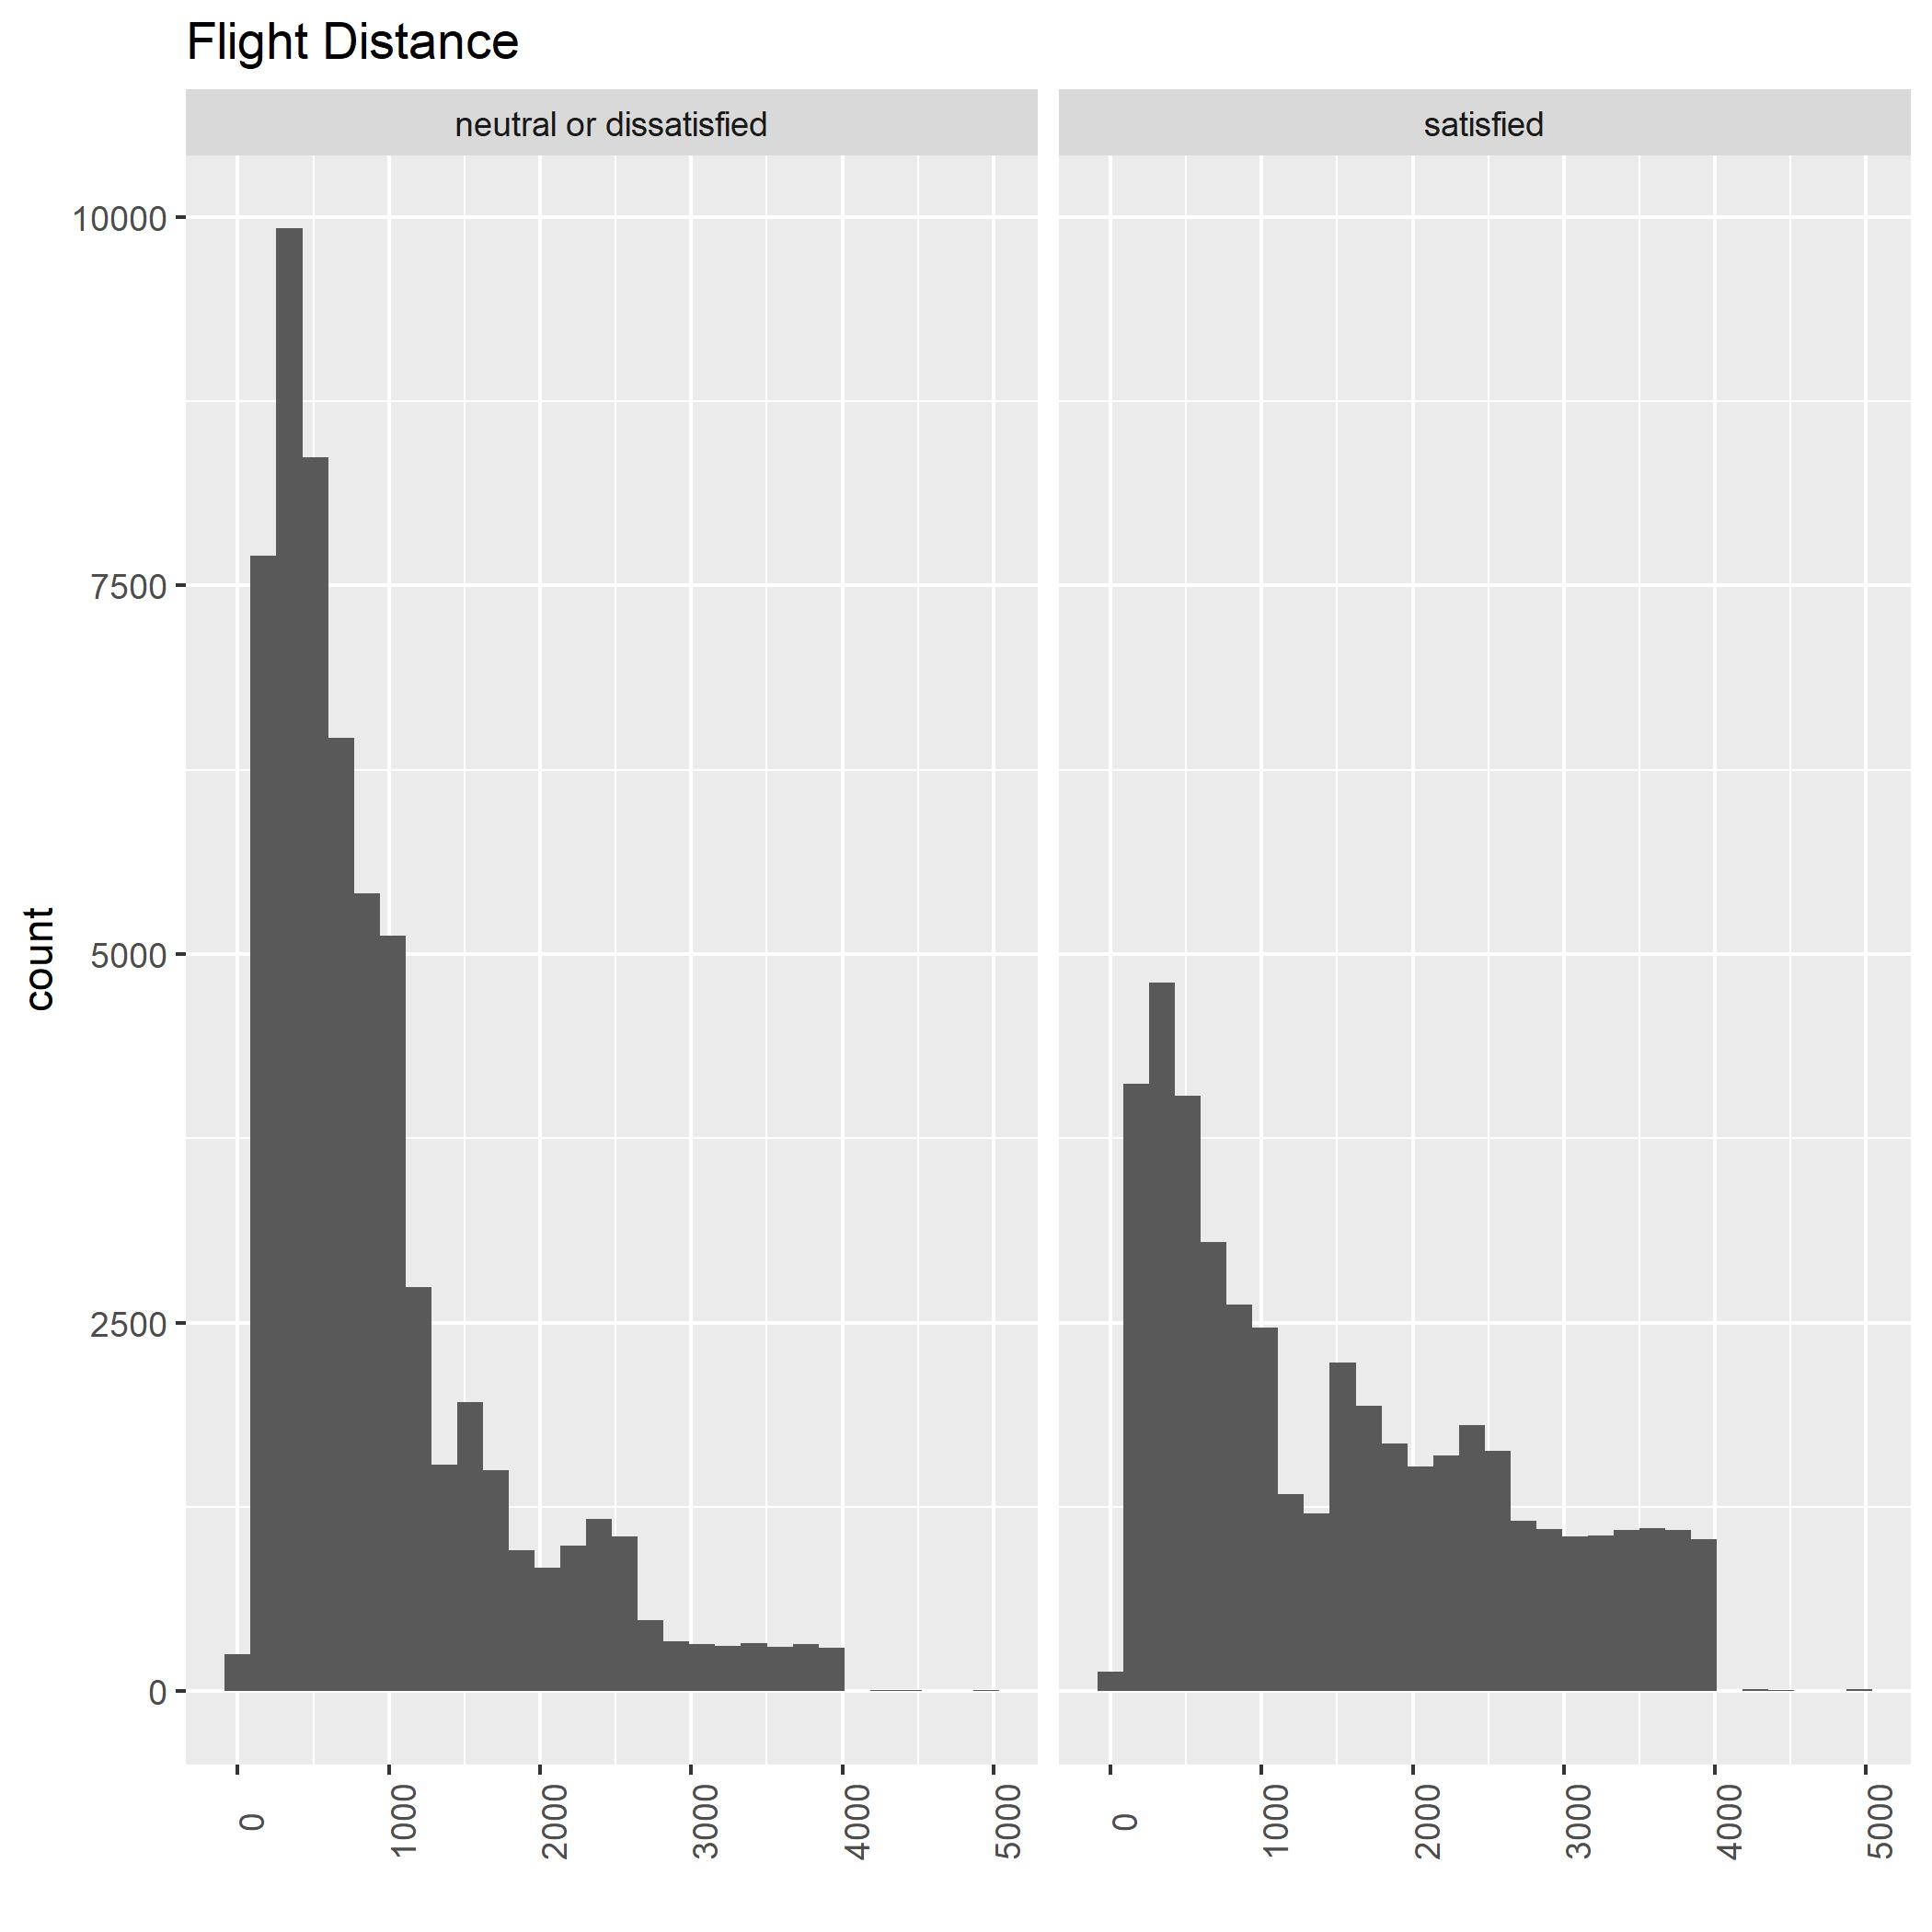
\includegraphics[width=.24\textwidth]{..//plots//plot6.jpg}\hfill
    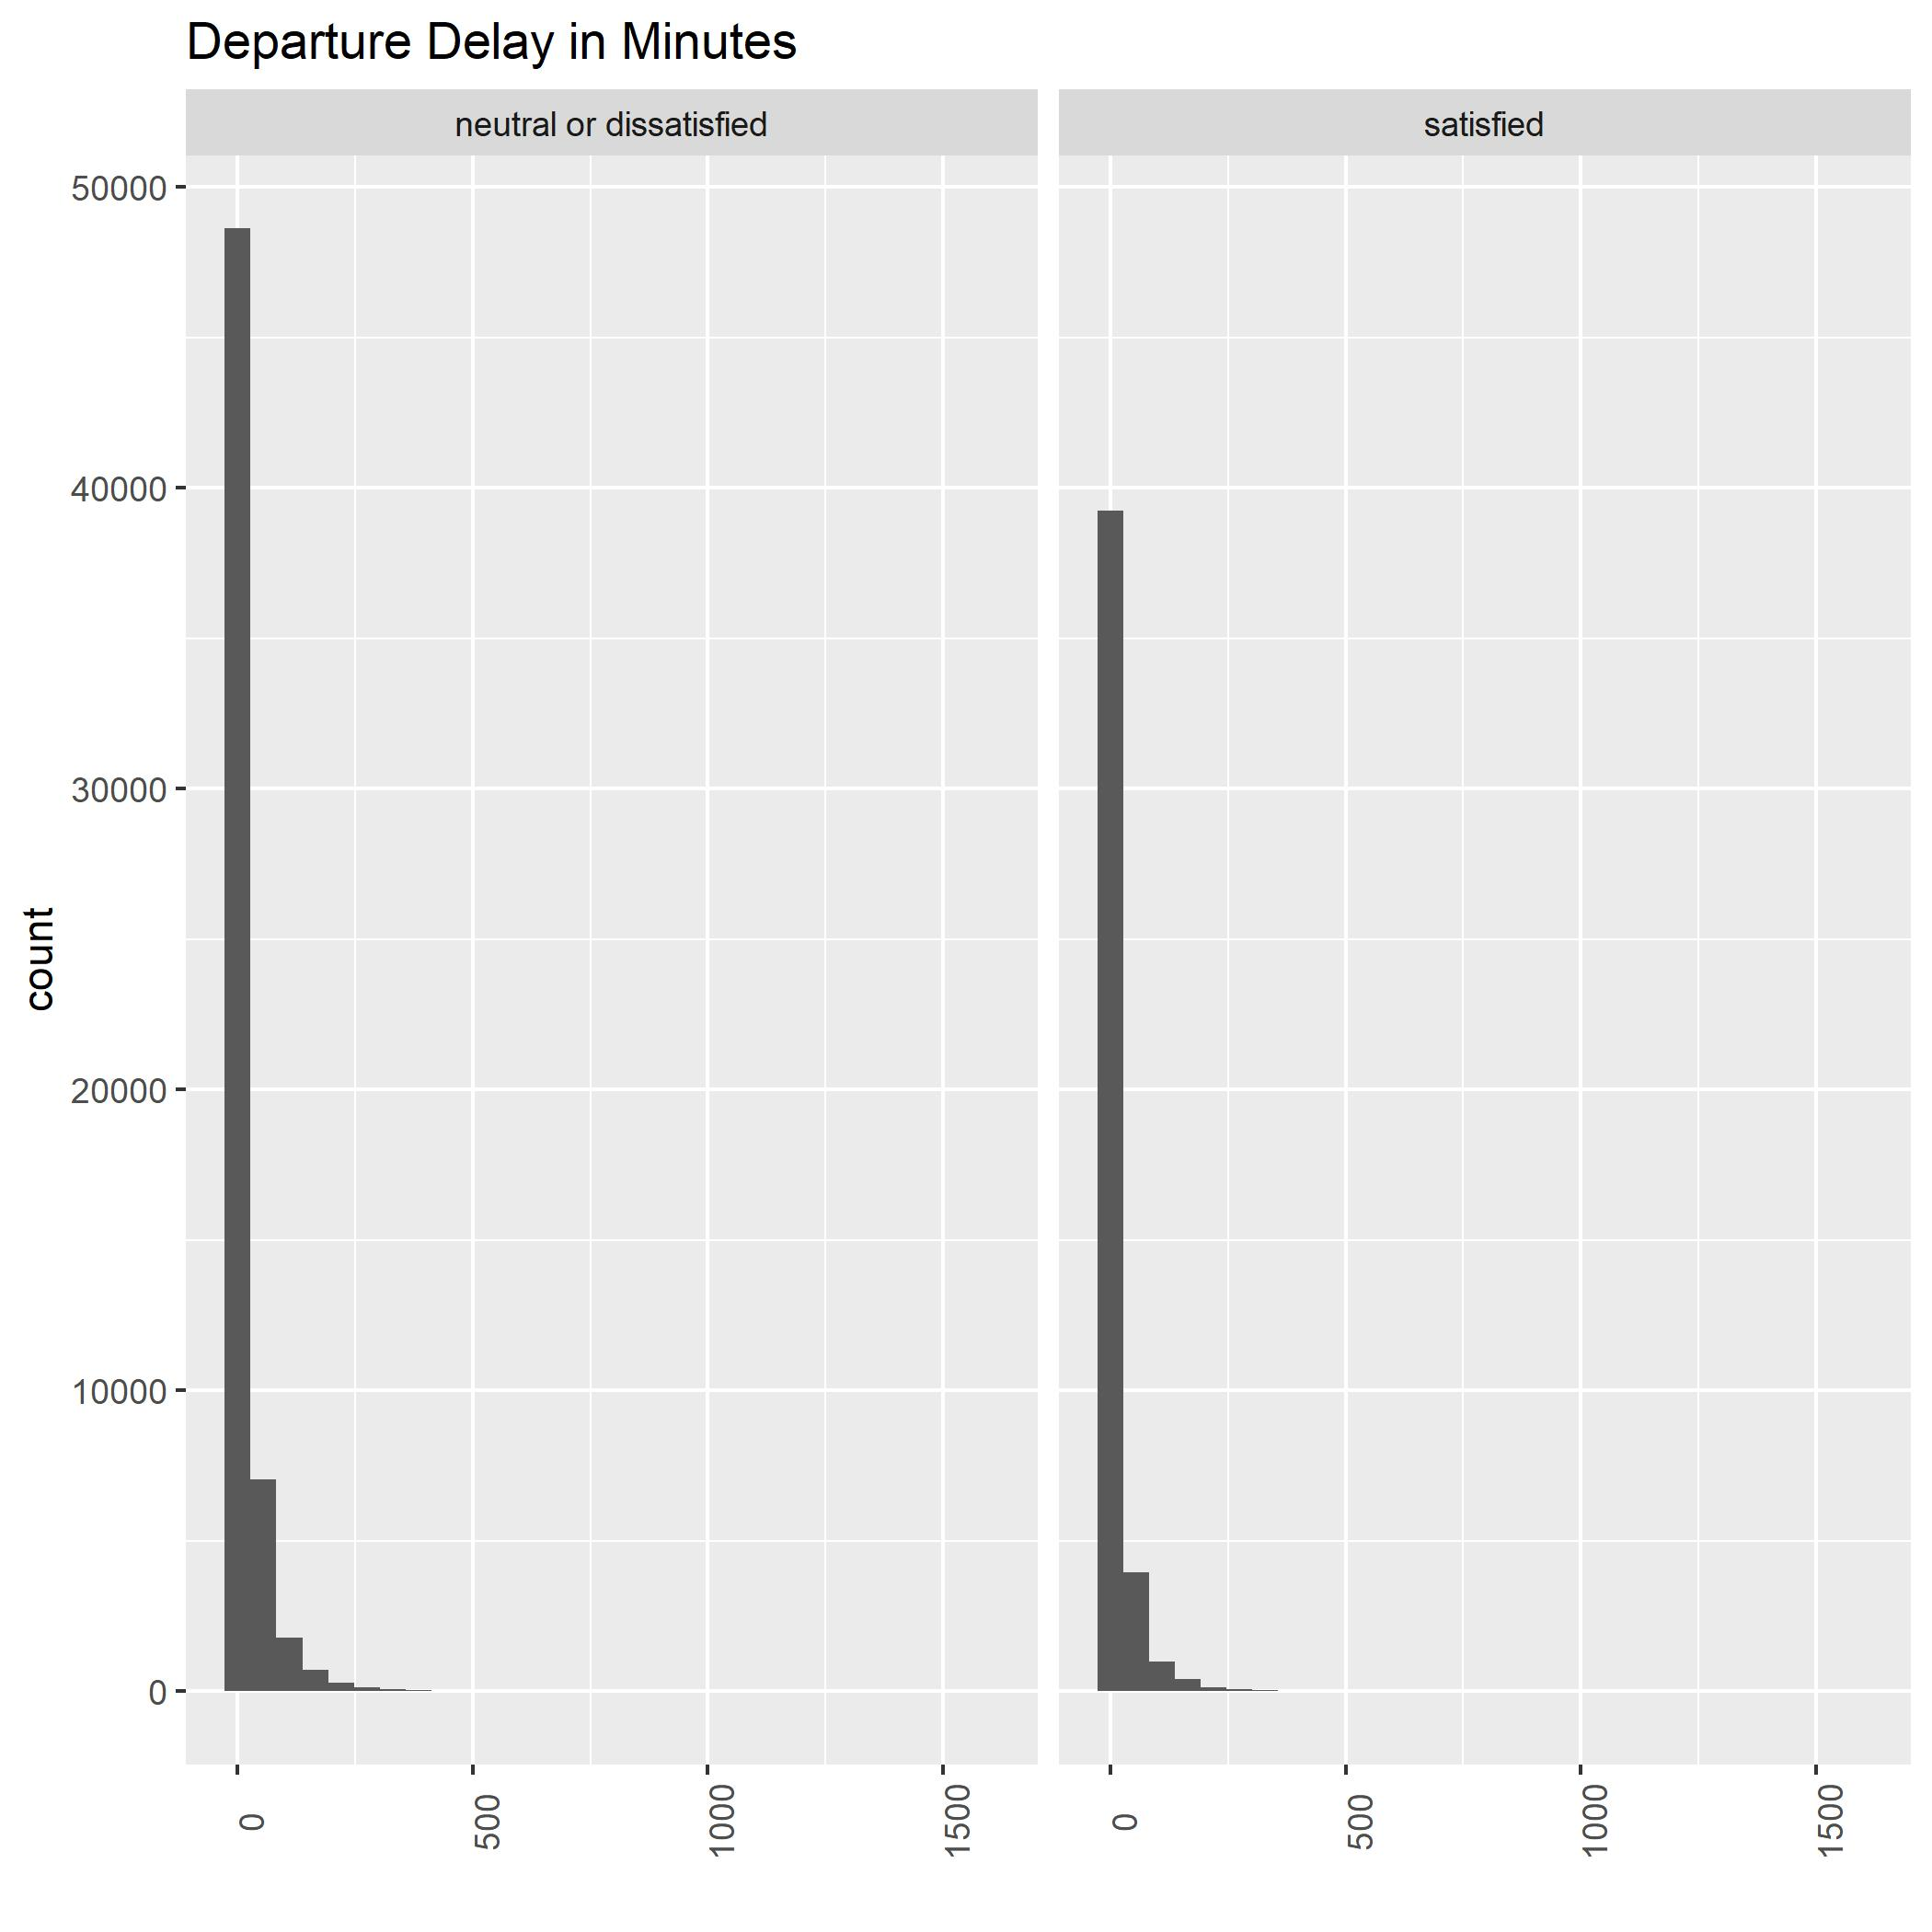
\includegraphics[width=.24\textwidth]{..//plots//plot21.jpg}\hfill
    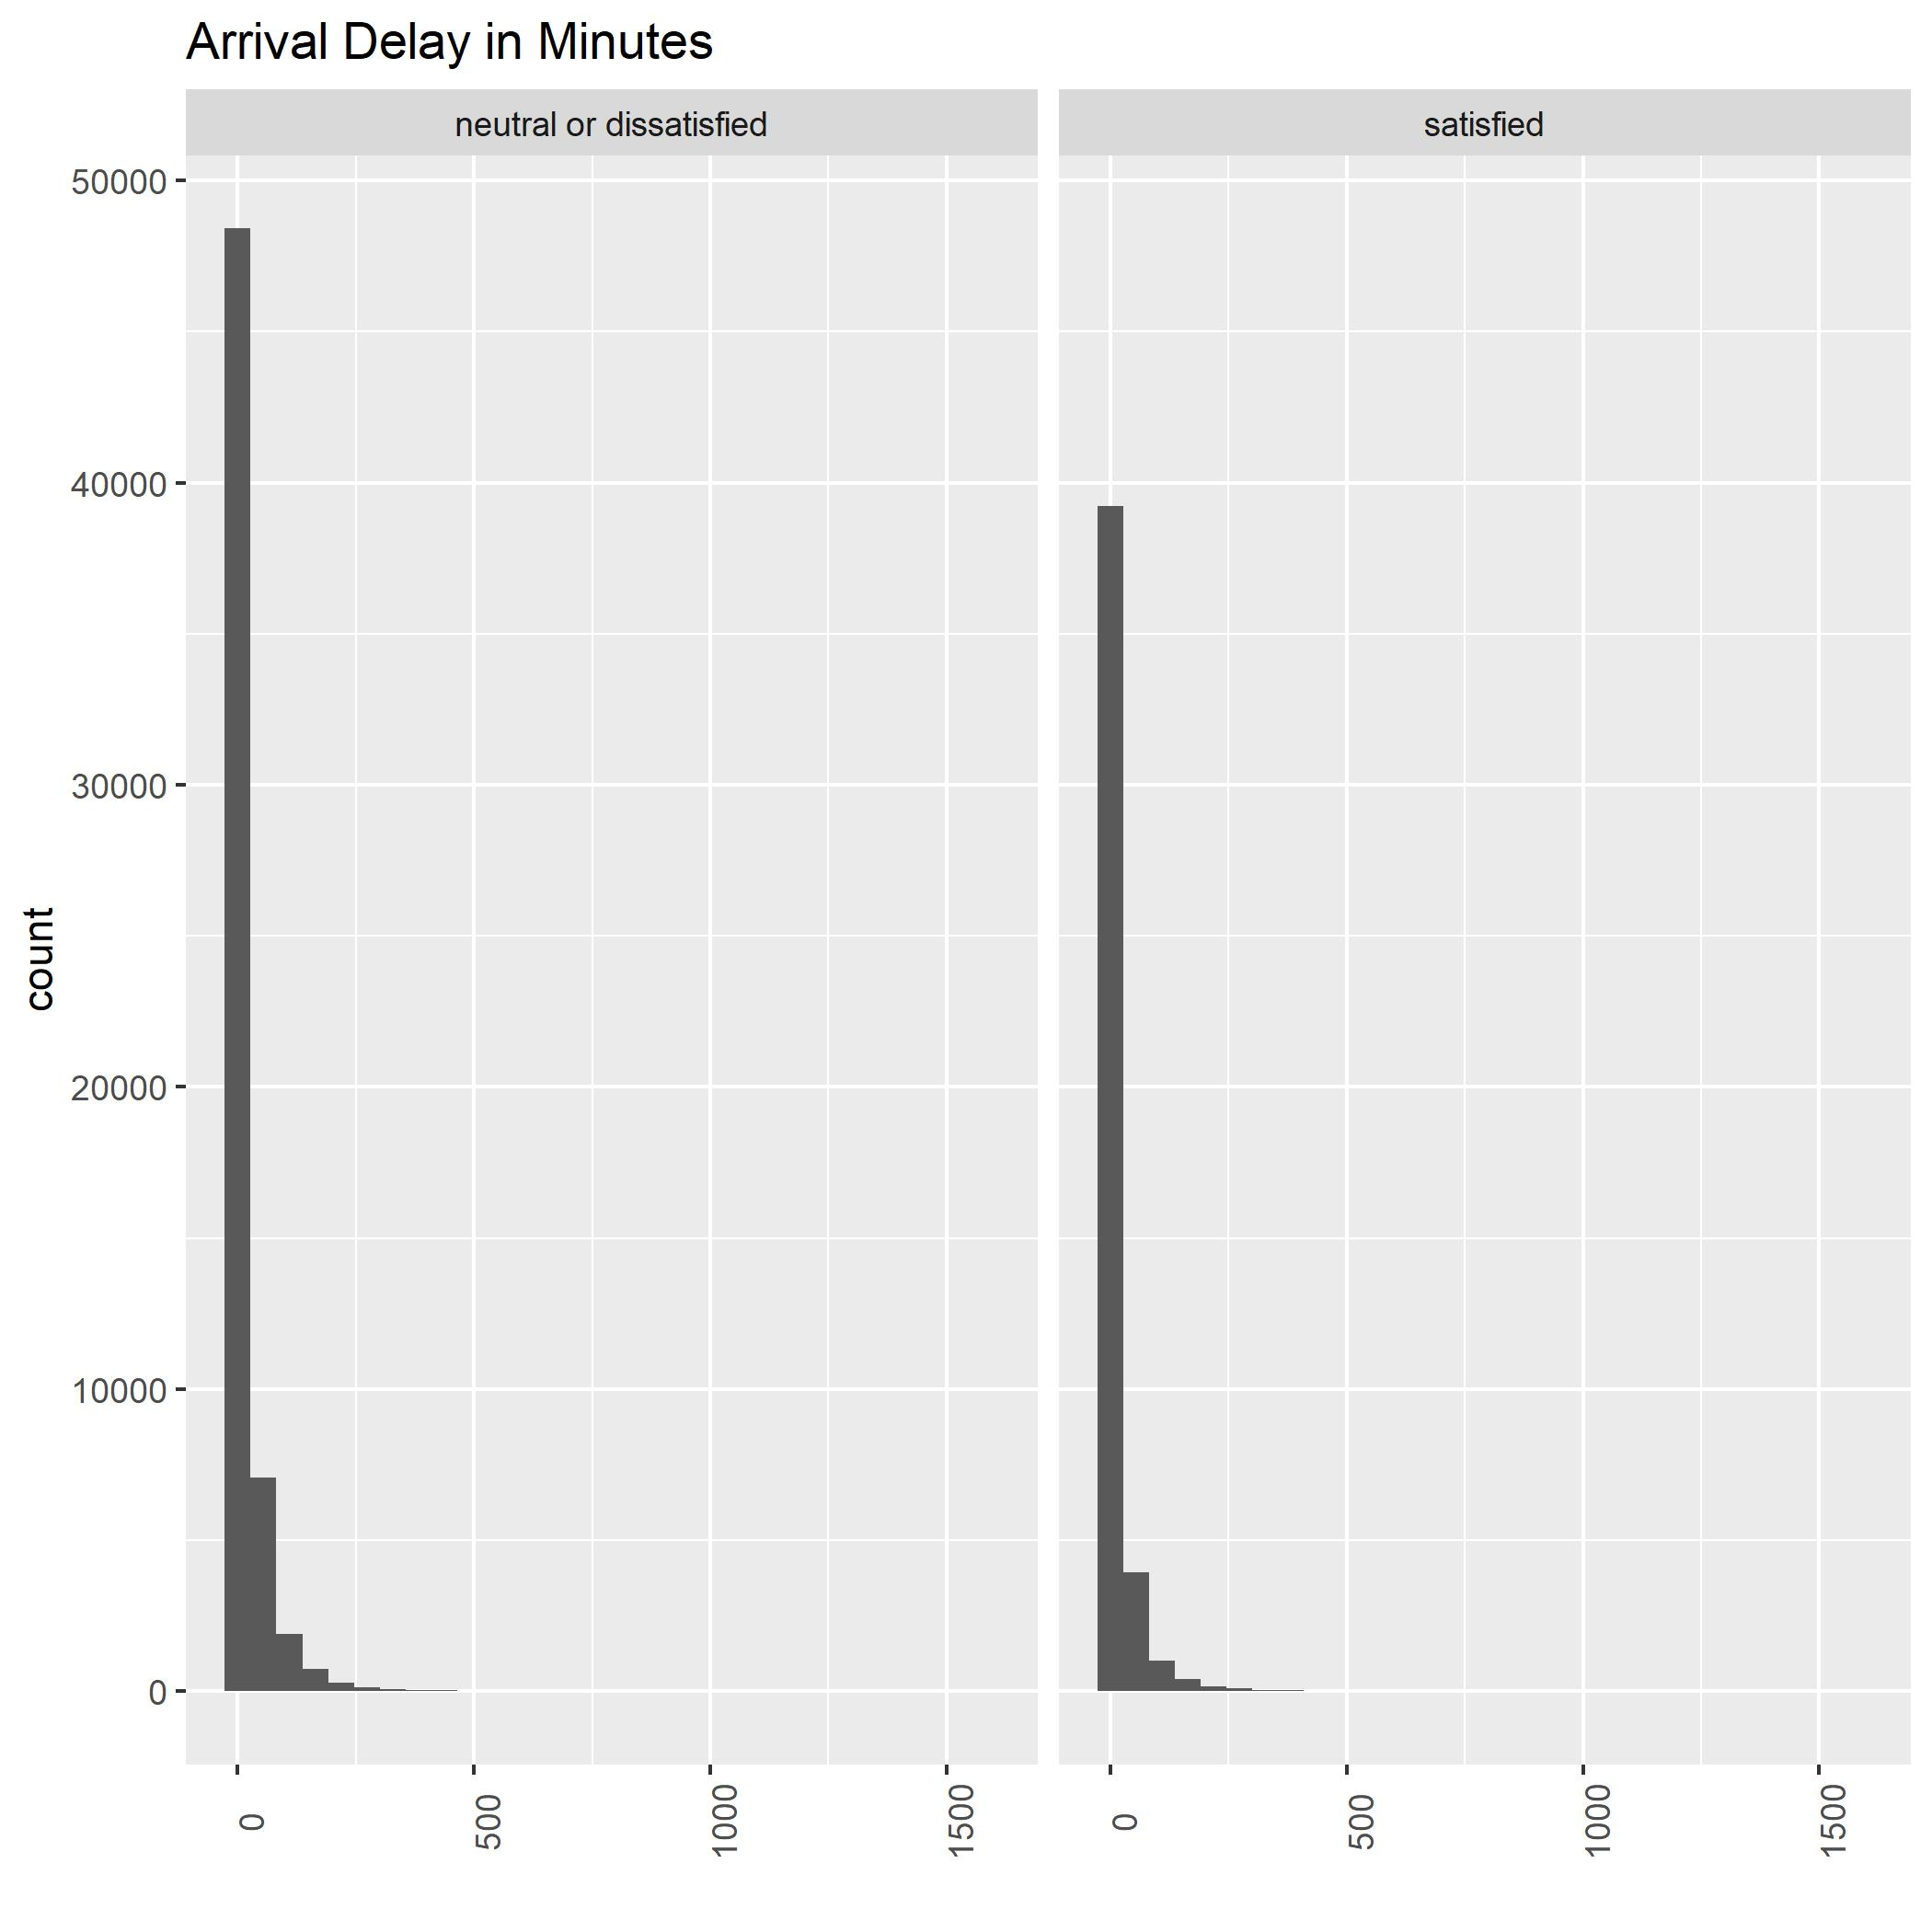
\includegraphics[width=.24\textwidth]{..//plots//plot22.jpg}\hfill
    \caption{Vizualisation of all intervall variables by criterion}\label{fig:foobar}
\end{figure}

\emph{Nominal variables}: Note: Some variables could also be considered
ordinal (E.g. Class). The genders are equally distributed in both the
``neutral or dissatisfied'' and in the ``satisfied'' box. This is a good
sign, since the data is likely to be a sample of a much larger database
itself. Of interest is the interaction between Type of Travel and
satisfaction. Where most of the ``Personal Travel'' customers are
dissatisfied, this cannot be said about the ``Business Travel''
customers. Comparing it with the plot for the class, this is a clear
hint, that the environment in Business Class leads to more satisfaction.
For interventions, this would be a good starting-point. \emph{Ordinal
variables}: 0 Means ``no answer'' given. For ordinal variables, to see
whether a variable has let to more satisfaction, the skewedness can be
interpreted: When both ``satisfied'' and ``neutral or dissatisfied''
plots" are left skewed, the variable is likely to not have a great
impact on the satisfaction rating (E.g. Departure time convenient).
Further, the height of the barplots can reveal information on the
factors that led to dissatisfaction. The heigher the ``neutral or
dissatisfied'' plot in oppose to the ``satisfied'' plot, the more an
item contributes to the dissatisfaction of the customers.\\
\emph{Interval variables}: Many of the plots are heavily skewed, which
must be considered when implementing the classifier. What is interesting
is, that especially younger people are dissatisfied. But my initial
hypothesis that younger people are more likely to travel in the ``Eco''
class is not really valid, since the correlation is -.13 (Age
\textasciitilde{} Class, Spearmans Rho; See Figure 4). So there must be
another reason.

\hypertarget{correlation-analysis}{%
\subsection{Correlation Analysis}\label{correlation-analysis}}

To extract teh variables that are likely to be associated with the
criterion (satisfaction), a correlation analysis is conducted. The
correlation coefficient is spearmans rho, which is made for correlation
of ordinal variables. Spearmans rho, in oppose to Pearson is a rank
correlation measure and is therefore, to a certain degree, also able to
detect non-linear relationships. Spearmans Rho was preferred over
Kendals Tau, because the dataset is rather large. Some say that Kendals
Tau does better on smaller datasets. There is quite a problem with a
correlation analysis since some variables are nominal. This must be
considered when interpreting the results.

Another problem with the correlation analysis at hand is, that there are
no significance measures included. Since there are 24 comparisons, using
p-values would likely lead to alpha inflation. Also, since the dataset
is rather large, even small correlation coefficinets are likely to get
significant. Bonferroni correcting the p-values would not be a good
idea, since there are 22 (!) single comparisons meaning alpha would be
0.05/22 = 0.002272727. A slight different approach is being chosen. The
correlation coefficient are evaluated against a well known/accepted
criterion of Cohen, 1988. According to this criterion, correlations
above +-0.5 are considered strong, correlations between +-0.3 and +- 0.5
are considered of medium strength and correlations between +-0.1 and
+-0.3 are considered of low strength. Correlations between -0.1 and -0.1
are considered as non existing.
(\url{https://www.scirp.org/(S(lz5mqp453edsnp55rrgjct55))/reference/ReferencesPapers.aspx?ReferenceID=2041144})
Interpretation with cohens` coefficients are of course not perfect and
do also come with limitations, but I think that they depict the reality
better than significance levels from correlation-tests.

Since spearmans rho does at least require ordinal ranks, correlating the
items that code a 0 as ``no answer'' would lead to biased correlation
coefficients (ordinal would mean, that 0 is worse than 1, which does not
hold true for our data). I controlled for this problem by recoding 0 as
NA and not using NAs for correlation (use = ``complete.obs'').
Considering that 0 does have a different meaning for ``Flight
Distance'', ``Departure Delay in Minutes'' and ``Arrival Delay in
Minutes'', these variables were not recoded with NA. Assumption for not
considering NAs: \textbf{Choosing ``no answer'' is compeletely at random
and does not have any relationship with satisfaction}

The results of the correlation analysis can be found in Tables 1 to 4.

According to the Cohen, 1988, online Boarding is most severely
associated with satisfaction rating. A good intervention would be to
further expand online checkin service.

Consult the heatmap in Figure 4 to get insights to intercorrelations.
Handle with care, since not all variables in there meet the requirements
of Spearmans Rho. The darker the color, the stronger the relationship.

\begin{figure}
  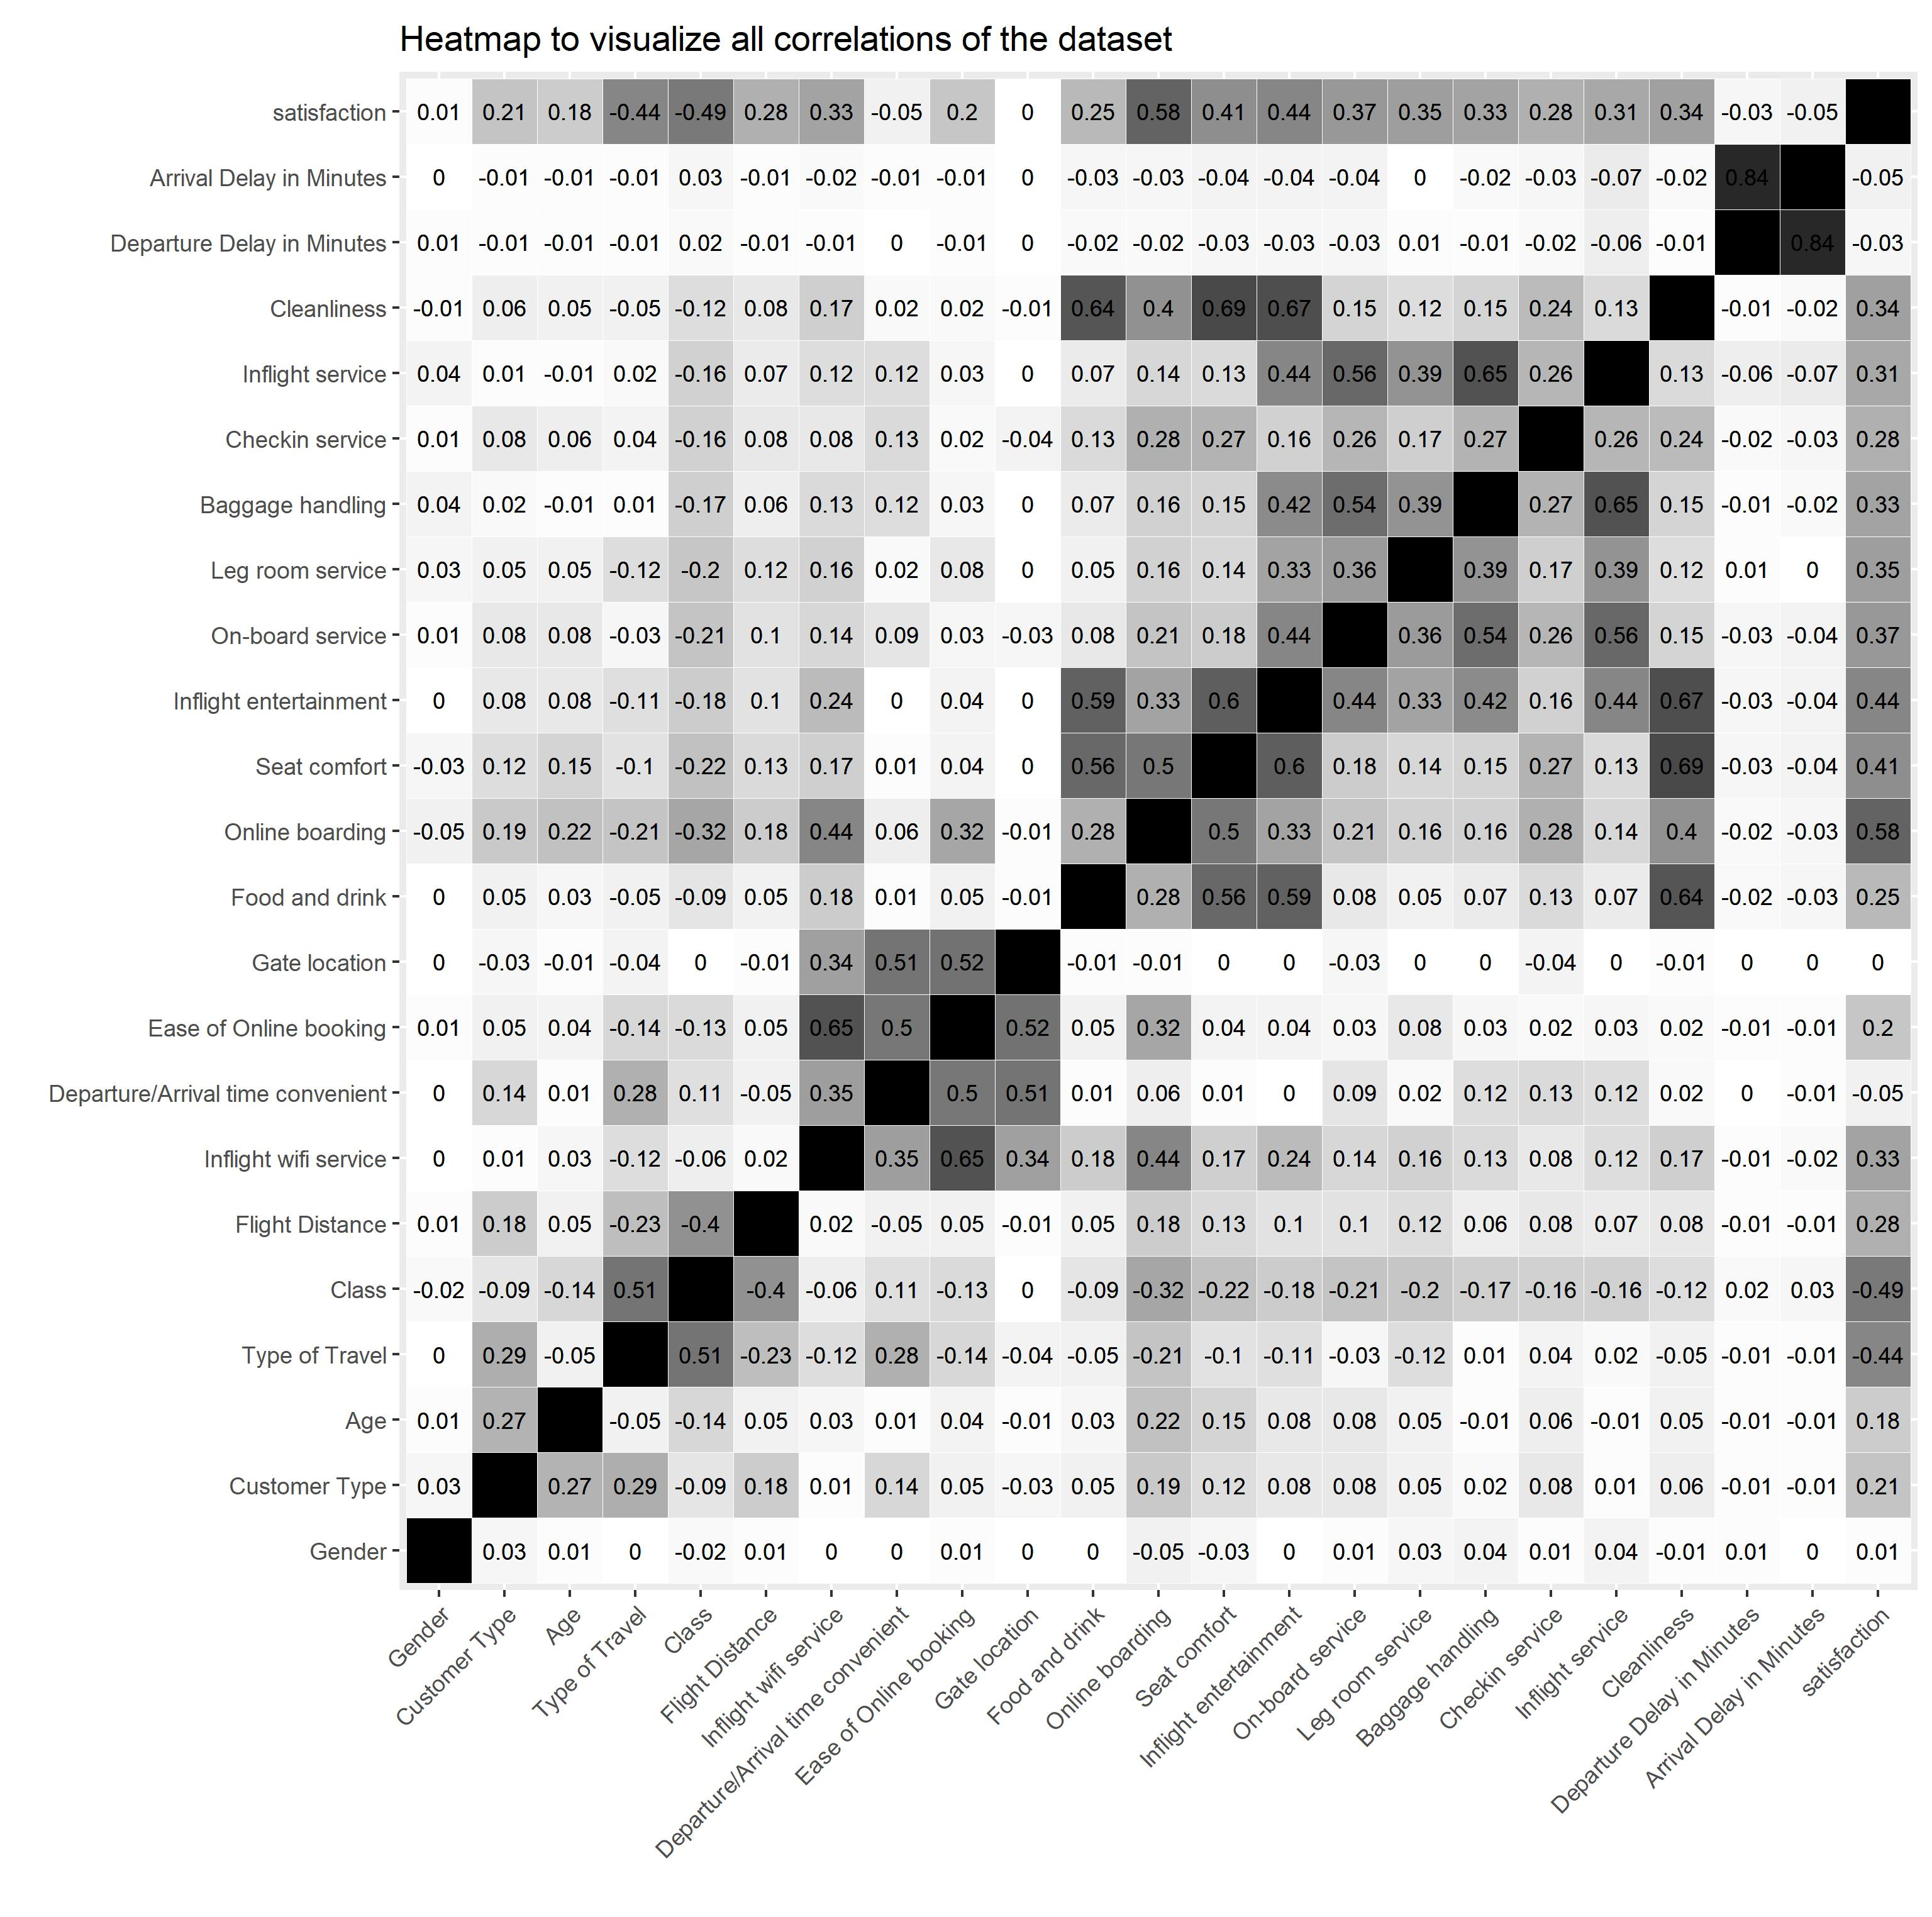
\includegraphics{..//plots//heatmap.jpg}
  \caption{The darker the color, the more significant the correlation. The correlation-coefficient is spearmans rho. Be careful with interpretation since there were nominal variables in there!}\label{fig:foobar}
\end{figure}

\begin{longtable}[]{@{}llr@{}}
\caption{correlations higher than +-0.5}\tabularnewline
\toprule
y & x & cor\tabularnewline
\midrule
\endfirsthead
\toprule
y & x & cor\tabularnewline
\midrule
\endhead
satisfaction & Online boarding & 0.5899783\tabularnewline
\bottomrule
\end{longtable}

\begin{longtable}[]{@{}llr@{}}
\caption{correlations between +-0.3 and +-0.5}\tabularnewline
\toprule
y & x & cor\tabularnewline
\midrule
\endfirsthead
\toprule
y & x & cor\tabularnewline
\midrule
\endhead
satisfaction & Type of Travel & -0.4489949\tabularnewline
satisfaction & Class & -0.4801065\tabularnewline
satisfaction & Inflight wifi service & 0.3722062\tabularnewline
satisfaction & Seat comfort & 0.3618708\tabularnewline
satisfaction & Inflight entertainment & 0.3995540\tabularnewline
satisfaction & On-board service & 0.3283335\tabularnewline
satisfaction & Leg room service & 0.3200487\tabularnewline
satisfaction & Cleanliness & 0.3031766\tabularnewline
\bottomrule
\end{longtable}

\begin{longtable}[]{@{}llr@{}}
\caption{correlations between +-0.1 and +-0.3}\tabularnewline
\toprule
y & x & cor\tabularnewline
\midrule
\endfirsthead
\toprule
y & x & cor\tabularnewline
\midrule
\endhead
satisfaction & Customer Type & 0.1875584\tabularnewline
satisfaction & Age & 0.1470610\tabularnewline
satisfaction & Flight Distance & 0.2573588\tabularnewline
satisfaction & Ease of Online booking & 0.2335138\tabularnewline
satisfaction & Food and drink & 0.2075063\tabularnewline
satisfaction & Baggage handling & 0.2693956\tabularnewline
satisfaction & Checkin service & 0.2323059\tabularnewline
satisfaction & Inflight service & 0.2654399\tabularnewline
\bottomrule
\end{longtable}

\begin{longtable}[]{@{}llr@{}}
\caption{items not associated with criterion (-0.1 and
0.1)}\tabularnewline
\toprule
y & x & cor\tabularnewline
\midrule
\endfirsthead
\toprule
y & x & cor\tabularnewline
\midrule
\endhead
satisfaction & Gender & 0.0123560\tabularnewline
satisfaction & Departure/Arrival time convenient &
-0.0468449\tabularnewline
satisfaction & Gate location & -0.0003662\tabularnewline
satisfaction & Departure Delay in Minutes & -0.0737981\tabularnewline
satisfaction & Arrival Delay in Minutes & -0.0735977\tabularnewline
\bottomrule
\end{longtable}

\hypertarget{exploratory-factor-analysis}{%
\subsection{Exploratory Factor
Analysis}\label{exploratory-factor-analysis}}

Since the task at hand asks for the factors that lead to customer
satisfaction, it would be interesting to see, whether some
variables/predictors are driven by ``higher'' factors. The appropriate
approach here would be to conduct an exploratory factor analysis, but
this is not possible since some variables are qualitative and various
other assumptions are not met. The approach chosen here is to conduct a
Factor Analysis for Mixed Data (FAMD), since this approach is capable of
working with qualitative and quantitative variables. The FAMD was
carried out using the FactoMineR and the factoextra package. A tutorial
can be found here:
\url{http://www.sthda.com/english/articles/31-principal-component-methods-in-r-practical-guide/115-famd-factor-analysis-of-mixed-data-in-r-essentials/}
FAMD is not really a Factor Analysis but rather a principal component
analysis. But due to the high similarity of the two, the interpretation
is rather similar. What has to be said though is that in pca, the
Dimensions are, unlike the factors in Factor Analysis, not uncorrelated.
This must be considdered when interpreting the results.

\begin{longtable}[]{@{}lrrr@{}}
\caption{Explained portion of variance by the principal
components}\tabularnewline
\toprule
& eigenvalue & variance.percent &
cumulative.variance.percent\tabularnewline
\midrule
\endfirsthead
\toprule
& eigenvalue & variance.percent &
cumulative.variance.percent\tabularnewline
\midrule
\endhead
Dim.1 & 4.095675 & 17.807284 & 17.80728\tabularnewline
Dim.2 & 2.374696 & 10.324765 & 28.13205\tabularnewline
Dim.3 & 2.204845 & 9.586283 & 37.71833\tabularnewline
Dim.4 & 1.971187 & 8.570377 & 46.28871\tabularnewline
Dim.5 & 1.836173 & 7.983361 & 54.27207\tabularnewline
\bottomrule
\end{longtable}

The results of the FAMD can be seen in Table 5 and in Figure 5. The
results are not really great. Capturing a total of 17.8 percent of the
total variance most likely leads to the interpretation that there are
not really overarching factors. But still, a look at the variables that
load primarely onto the first 4 dimensions cannot be a bad idea (Figure
6)

\begin{figure}
  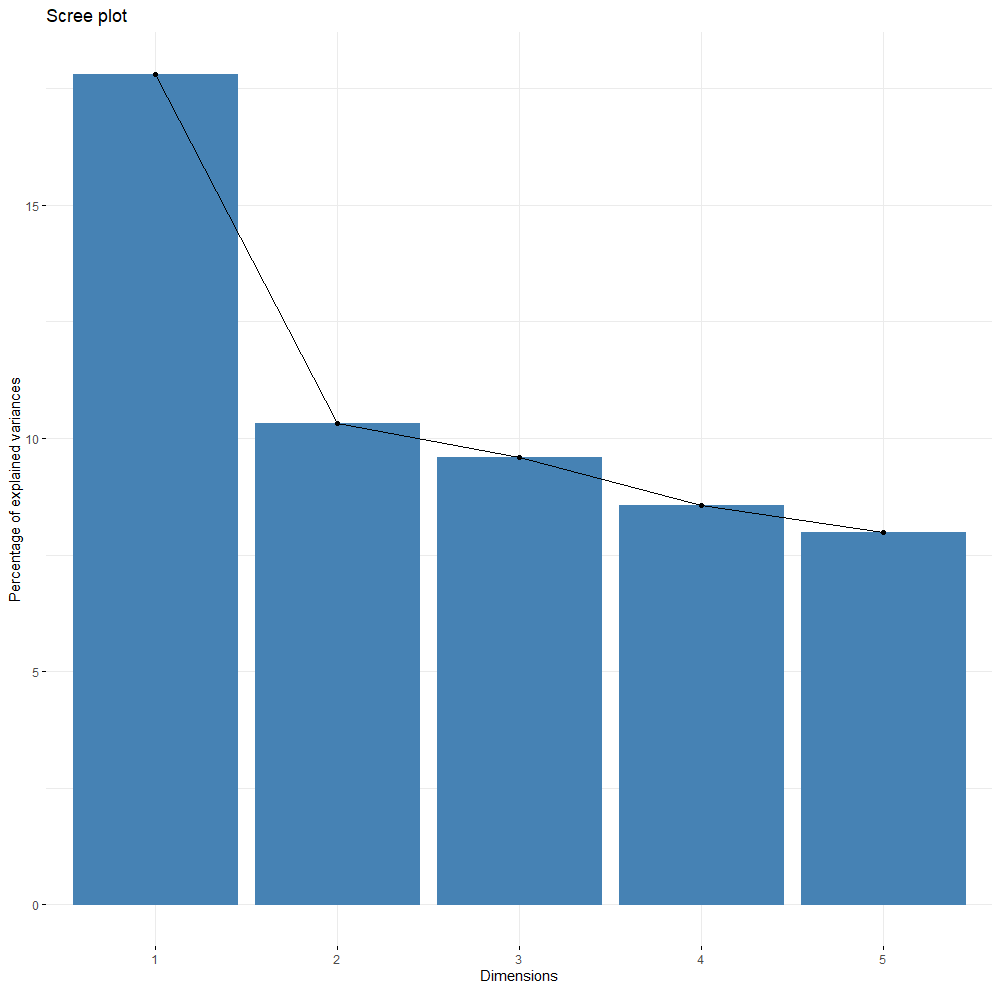
\includegraphics[width=.48\textwidth]{..//plots//screeplot.png}
  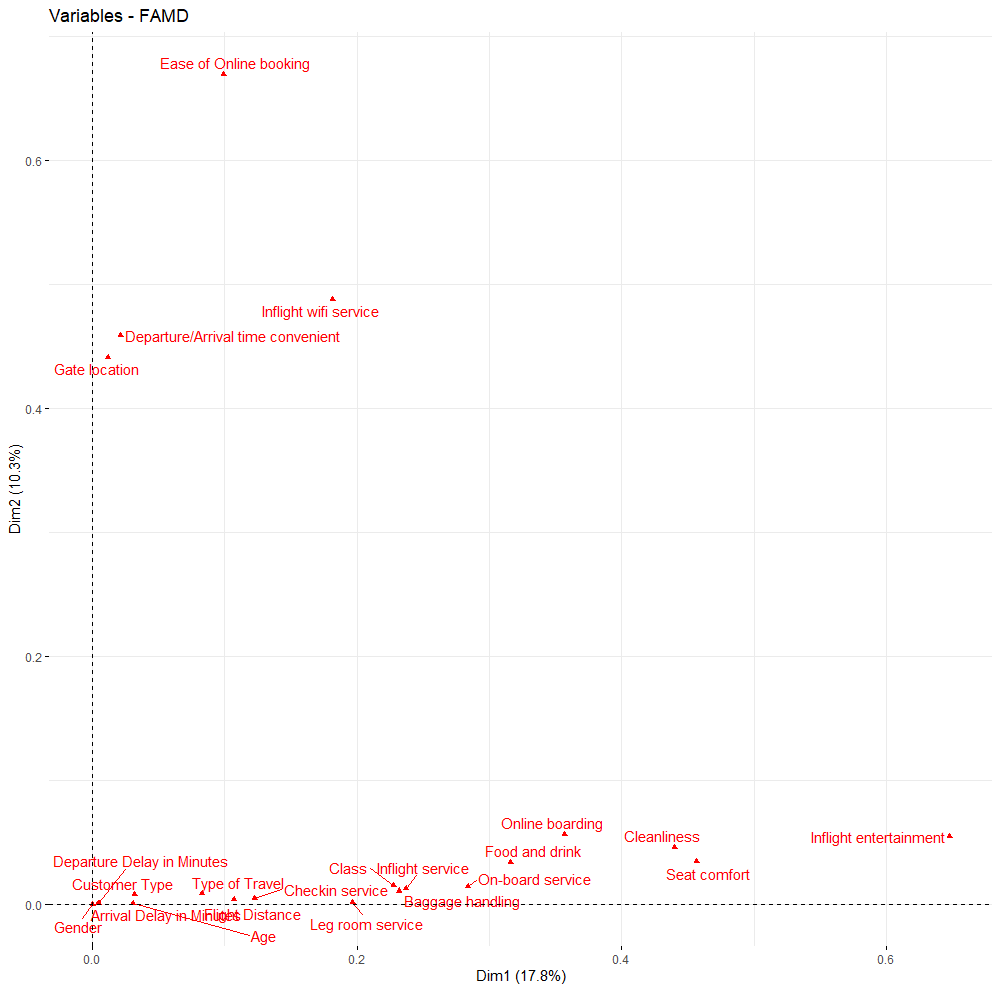
\includegraphics[width=.48\textwidth]{..//plots//fact1.png}
  \caption{Left: Screeplot of FAMD: Traditionally one would only accept dimension 1, but variance on this dimension is really small; Right: The variables plotted on the first two dimensions}\label{fig:foobar}
\end{figure}

\begin{figure}
  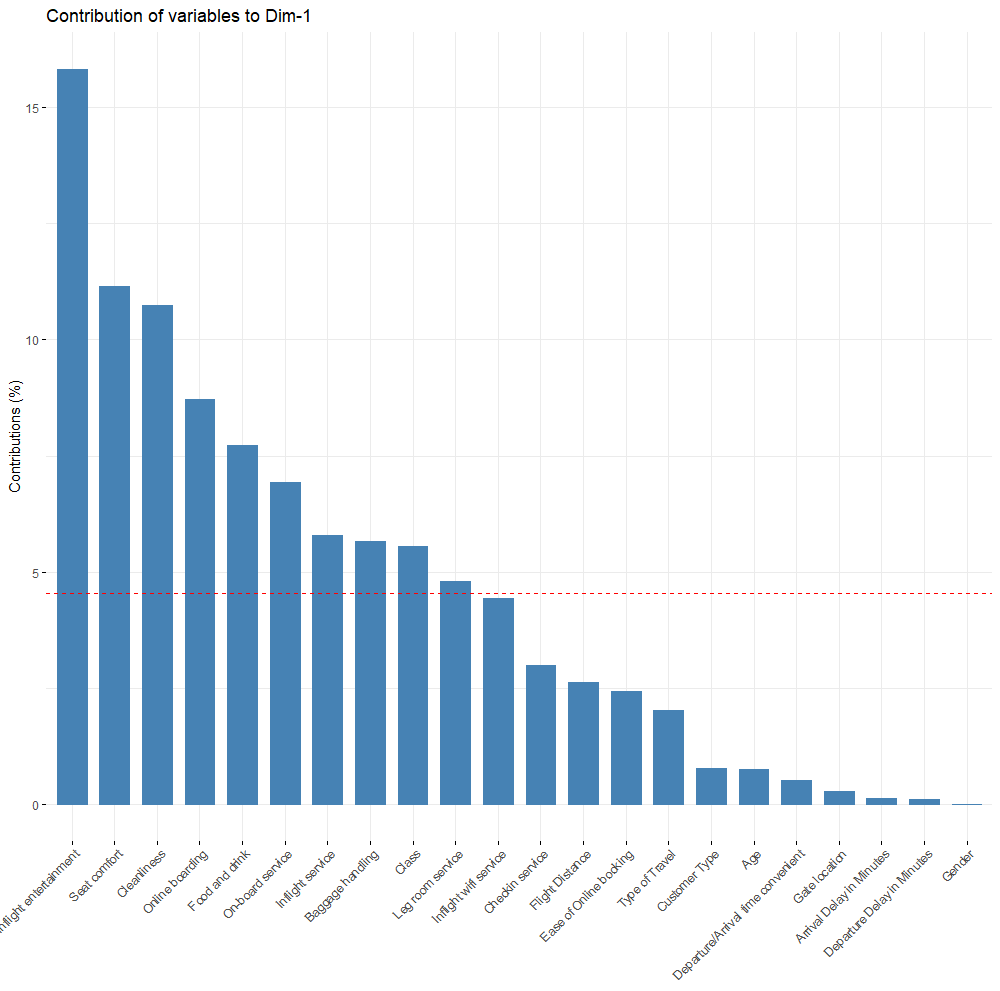
\includegraphics[width=.24\textwidth]{..//plots//fact2.png}
  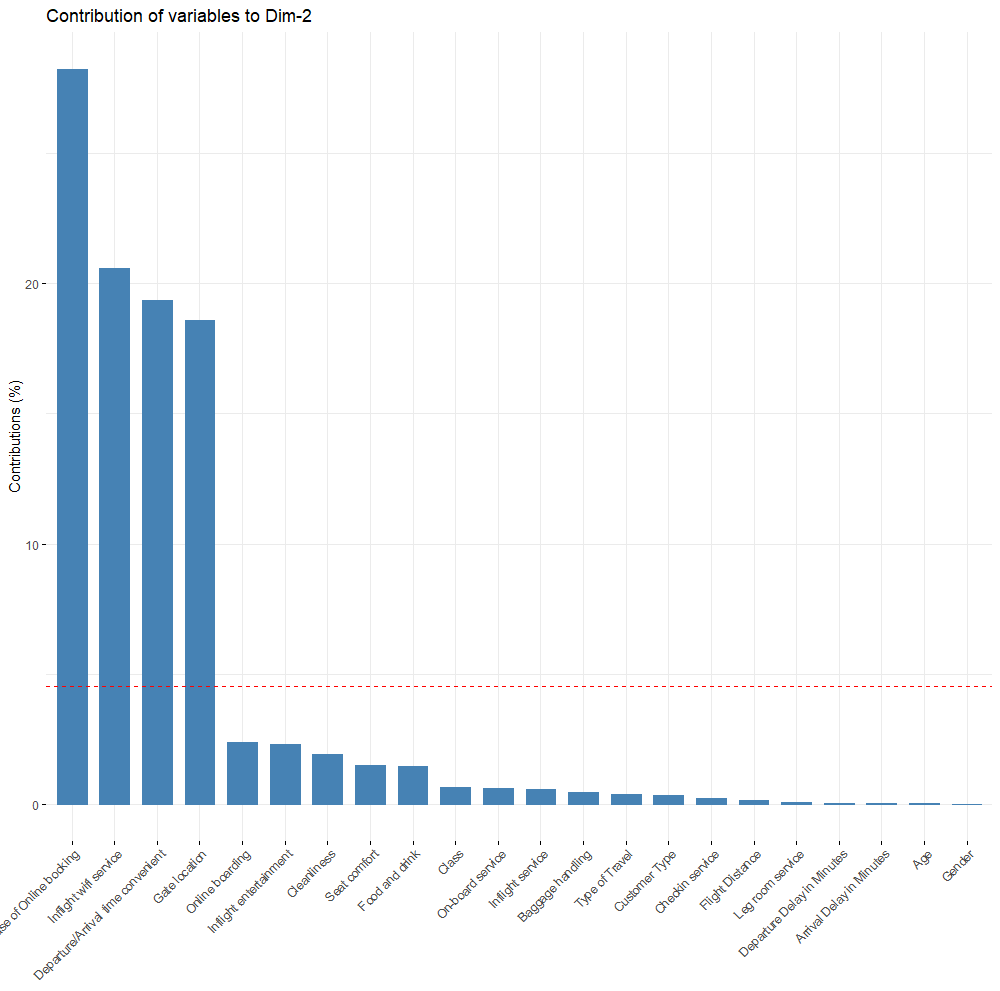
\includegraphics[width=.24\textwidth]{..//plots//fact3.png}
  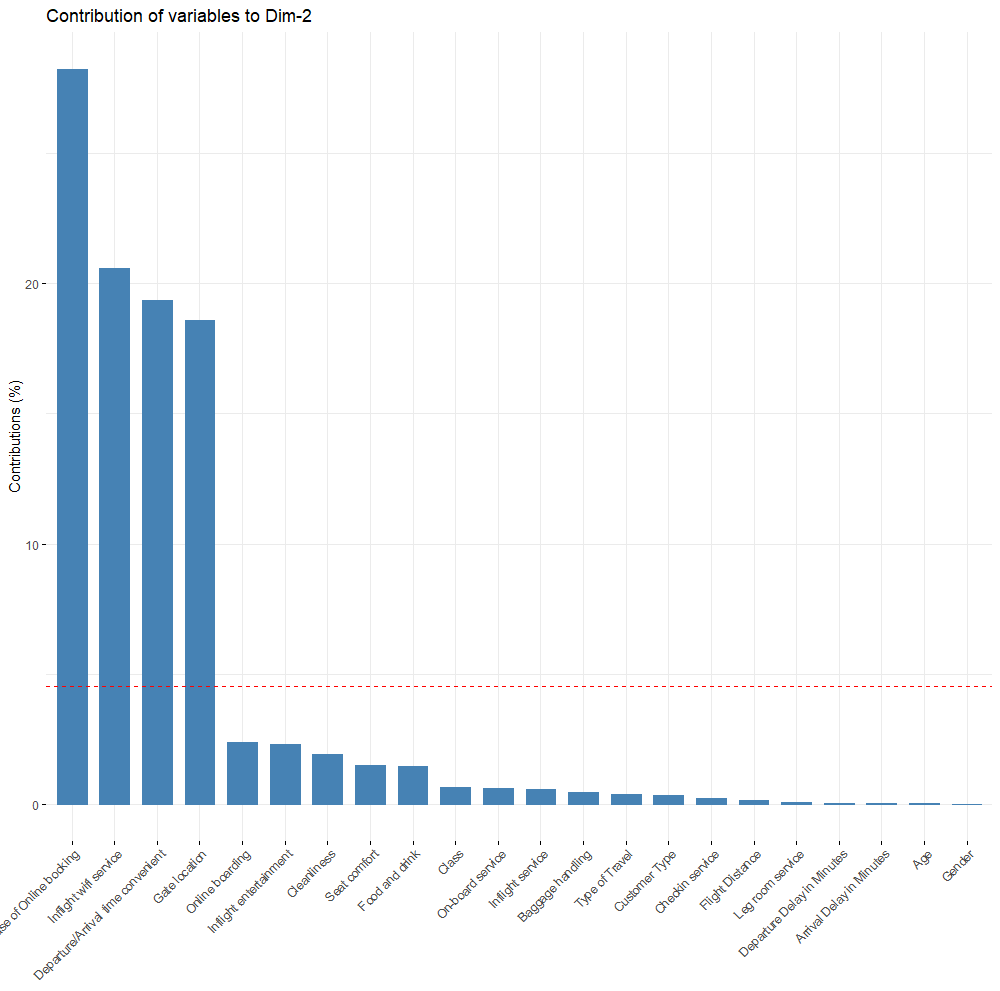
\includegraphics[width=.24\textwidth]{..//plots//fact3.png}
  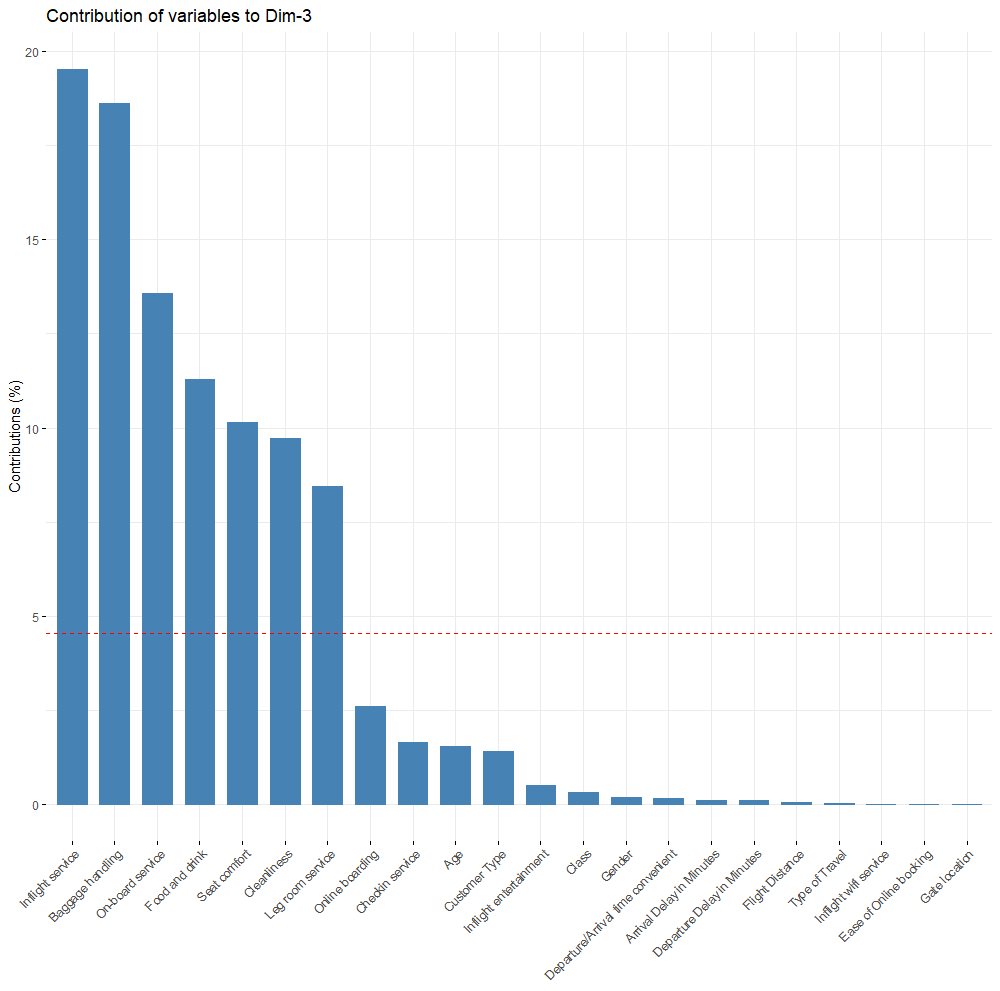
\includegraphics[width=.24\textwidth]{..//plots//fact4.png}
  \caption{Zoom in to see more. The variables that load to the first 4 dimensions. The red dashed line on the graph above indicates the expected average value, if the contributions were uniform.}\label{fig:foobar}
\end{figure}

As stated above the validity of an interpretation of the dimensions is
vastly in doubt. However, here are possible Factors that the first two
dimensions might cover (Note again that the dimensions are NOT
uncorrelated and some items load on more than one dimension):

\begin{itemize}
\item
  \textbf{Dimension 1}: Inflight entertainment, Seat comfort,
  Cleanliness, Online boarding, Food and drink, On-board service,
  Inflight service, Baggage handling, Class, Leg room service.
  \textbf{Interpretation}: These are mostly variables that concern
  inflight services and inflight personal confort.
\item
  \textbf{Dimension 2}: Ease of online booking, Inflight wifi service,
  Arrival/Departure time convenient, Gate location.
  \textbf{Interpretation}: These are mostly variables that concern
  factors that surround the flight.
\end{itemize}

Conclusion: FAMD is not really useful here and no conclusion can be
drawn from the results.

\hypertarget{machine-learning-for-deeper-insights.}{%
\subsection{Machine Learning for Deeper
Insights.}\label{machine-learning-for-deeper-insights.}}

With the dataset at hand an the task concerning it, it is actually not
ideal to use a model that maximized accuracy but is not interpretable.
However, the assignment, this report is for, requires to maximize
accuracy, so the modelling here is split into two parts: First there
will be a discussion of decision trees, which also includes in
interpretation for the task. Second there will be an accuracy optimising
part, where ensemble methods (all treebased) were implemented to
maximize predictive validity. These models cannot directly be used for
interpretation, since they are blackbox models (at least the boosting
method).

\hypertarget{cross-validation}{%
\subsubsection{Cross Validation}\label{cross-validation}}

The data was first split into a training dataset and a testing dataset
(80\% vs.~20\%). The training dataset was further split into ten folds.
Therefore, to improve model robustness \textbf{10 fold cross validation}
was used. After the model fit was estimated, it got benchmarked on the
training dataset (in-sample) and the testing dataset (out-of-sample).
The model fit has never seen the data from the testing dataset. The
10-fold cross validation technique could have been further extended with
a repeated cross validation. However, since I wanted to use the same
validation technique for all my models and because the ensemble methods
were already computationally expensive themselves, I did decide against
it.

All models were fitted in parallel. All models were implemented using
the caret package.

\hypertarget{decision-tree-analysis}{%
\subsubsection{Decision tree analysis}\label{decision-tree-analysis}}

A decision tree seems appropriate for the task. Decision trees have
several benefits: They are insensitive to outliers (so no outlier
detection was carried out), they are insensitive to skewed data (so no
transformations were used) and they work well with mixed data (nominal,
ordinal and interval). Further, decision trees are easily to interpret,
which is important for finding interventions for the airline company. It
is also good to mention, that decision trees exploit variables by their
predictive validity and do automatically exclude variables, that are not
of further use. Therefore, no variables were excluded as predictors. The
final tree provided an accuracy of 0.8441 in-sample and 0.8407
out-of-sample, which is acceptable considering the a priori probability
of 0.56.

Since decision trees exploit variables as much as possible, they contain
information on the importance of the variables. The variables were
ranked as follows:

\begin{longtable}[]{@{}rl@{}}
\caption{Variables with the most importance}\tabularnewline
\toprule
Rank & Variable\tabularnewline
\midrule
\endfirsthead
\toprule
Rank & Variable\tabularnewline
\midrule
\endhead
1 & Online Boarding\tabularnewline
2 & Seat Comfort\tabularnewline
3 & Inflight Wifi Service\tabularnewline
4 & Type of Travel\tabularnewline
5 & Class\tabularnewline
\bottomrule
\end{longtable}

Online Boarding (neutral or dissatisfied when Online Boarding
\textless{} 4) and Type of Travel (Personal Travel (2) leads to neutral
or dissatisfied) represent the two primary nodes. This can be used to
make the decision about what the intervention will look like: Improving
Online Boarding would probably lead to great improvement of the
satisfaction rating. Type of Travel might mean, that the conditions for
personal travel are not really good, interventions in this regard would
also improve the satisfaction rating. The output (Figure 7) further
shows, that when customers travel in the Eco class, they also state that
they are dissatisfied. Improving conditions in this class, would
therefore lead to better satisfaction ratings.

\begin{figure}
  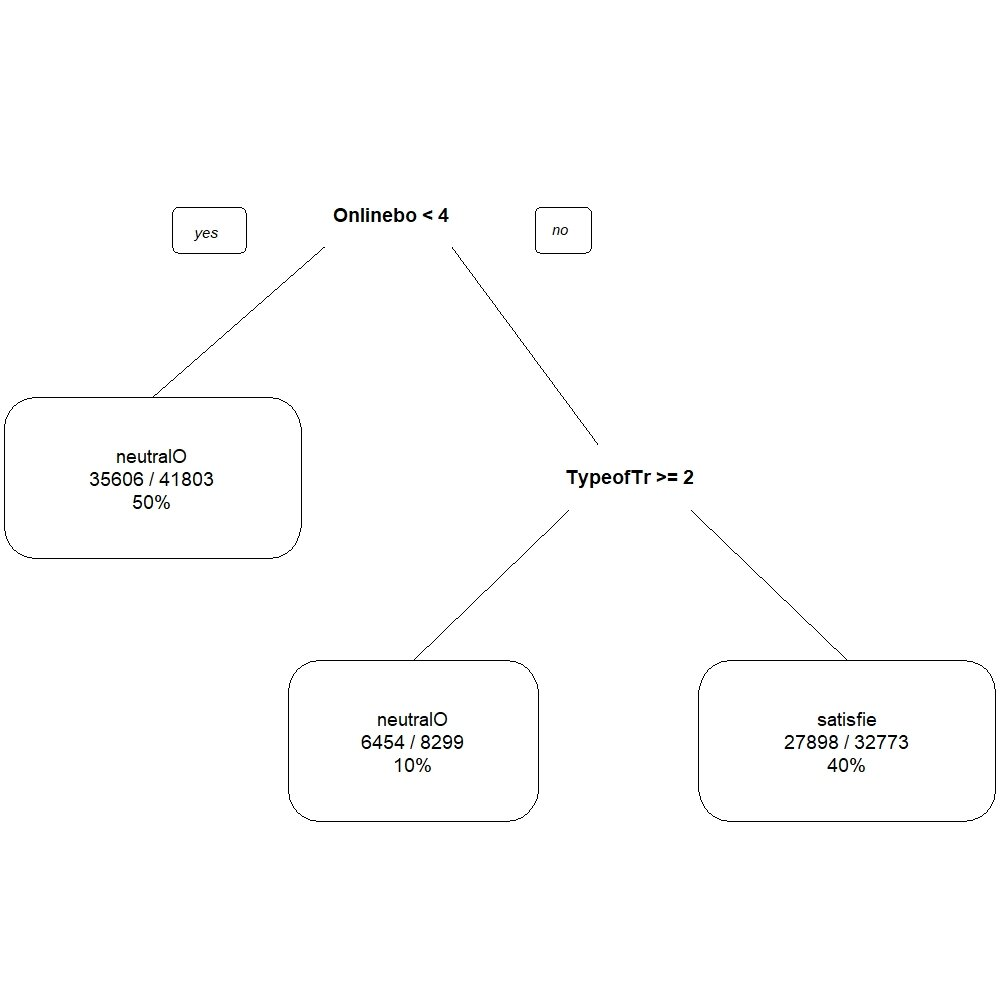
\includegraphics[width=.48\textwidth]{..//plots//decisiontree.jpg}
  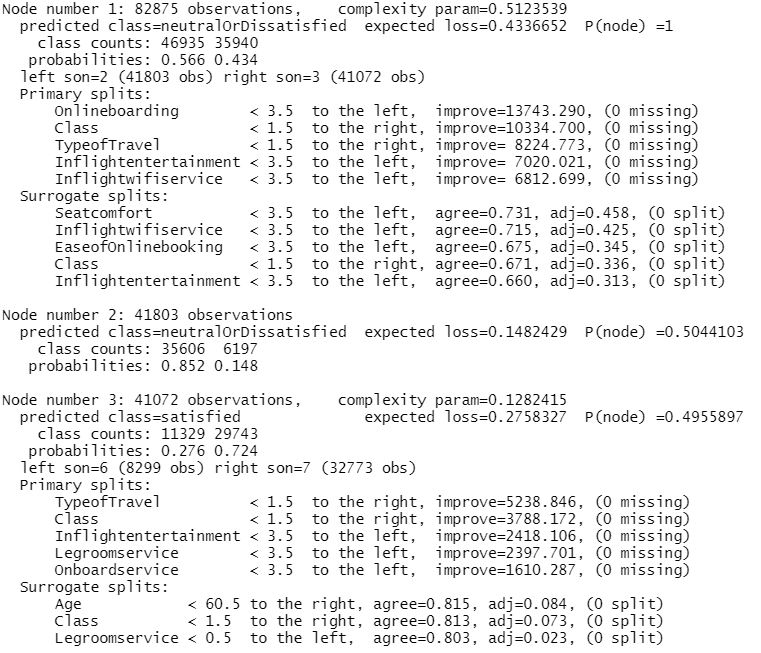
\includegraphics[width=.48\textwidth]{..//plots//outputdecisiontree.jpg}
  \caption{Left: Decision tree: For the split with TypeofTravel, the Class-variable could also be used; Right: Extensive overview on the decision rules}\label{fig:foobar}
\end{figure}

\hypertarget{improving-accuracy-with-ensemble-methods.}{%
\subsubsection{Improving Accuracy With Ensemble
Methods.}\label{improving-accuracy-with-ensemble-methods.}}

For improving accuracy, I still wanted to stick to tree based methods.
Therefore, I used random forest as a bagging approach and gradient
boosting sequential trees as a boosting approach.

\hypertarget{random-forest}{%
\paragraph{Random Forest}\label{random-forest}}

The random forest was estimated using the Rborist package in caret which
holds a very efficient approach to random forests (Breiman, L. (2001).
Random forests. Mach Learn, 45:5-32.
\url{https://doi.org/10.1023/A:1010933404324}.). To further improve the
speed of the estimation, I did not use the formula specification but
rather entered the predictors and the criterion directly. This is
recommended in various forums. The Rborist function holds two parameters
that were automatically tuned. Therefore, no further specification was
needed. The best values are: predFixed = 22 and minNode = 2. The random
forest was able to get an accuracy of 0.9734 in sample and an accuracy
of 0.9745 out of sample.

\hypertarget{gradient-boosting-sequential-trees.}{%
\paragraph{Gradient Boosting Sequential
Trees.}\label{gradient-boosting-sequential-trees.}}

Gradient boosting sequential trees were implemented using the gbm
package in caret. The model has 4 parameters, two of them are hold
constant by default. To vary them as well, I specified custom values for
all parameters. The best values estimated by the model for the 4
parameters are: n.trees: 250, interaction.depth = 7, shrinkage = 0.15
and n.minobsinnode = 15. For all parameters the maximum value specified
in advance (in the gradientboostgrid) was chosen. I think that accuracy
could be further improved by allowing the model higher values in all
parameters. However, higher values, for example, in the n.trees
parameter will increase computation times by quite a bit, which is why I
have not re-estimated the model. The gradient boosting sequential trees
were able to achieve an accuracy of 0.9624 in sample and an accuracy of
0.9615 out of sample. Therefore, they benchmark slightly worse than the
random forest. I assume that with better parameters, they could beat the
random forest.

\hypertarget{model-selection.}{%
\paragraph{Model Selection.}\label{model-selection.}}

For selecting the best model, boxplots of the 10 folds (from cross
validation) of all tree models were compared. For both Kappa and
Accuracy, the Gradient boosting sequential trees seem to be slightly
better than the random forest. However, the random forest did slightly
better in the in-sample and out-of-sample accuracy. Deciding for the
best model is therefore rather a coin flip.

\begin{figure}
  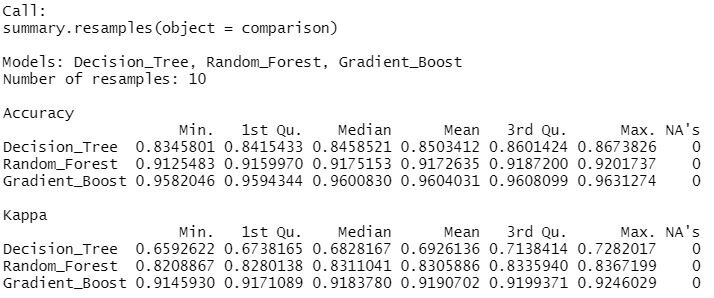
\includegraphics[width=.48\textwidth]{..//plots//comparison.jpg}
  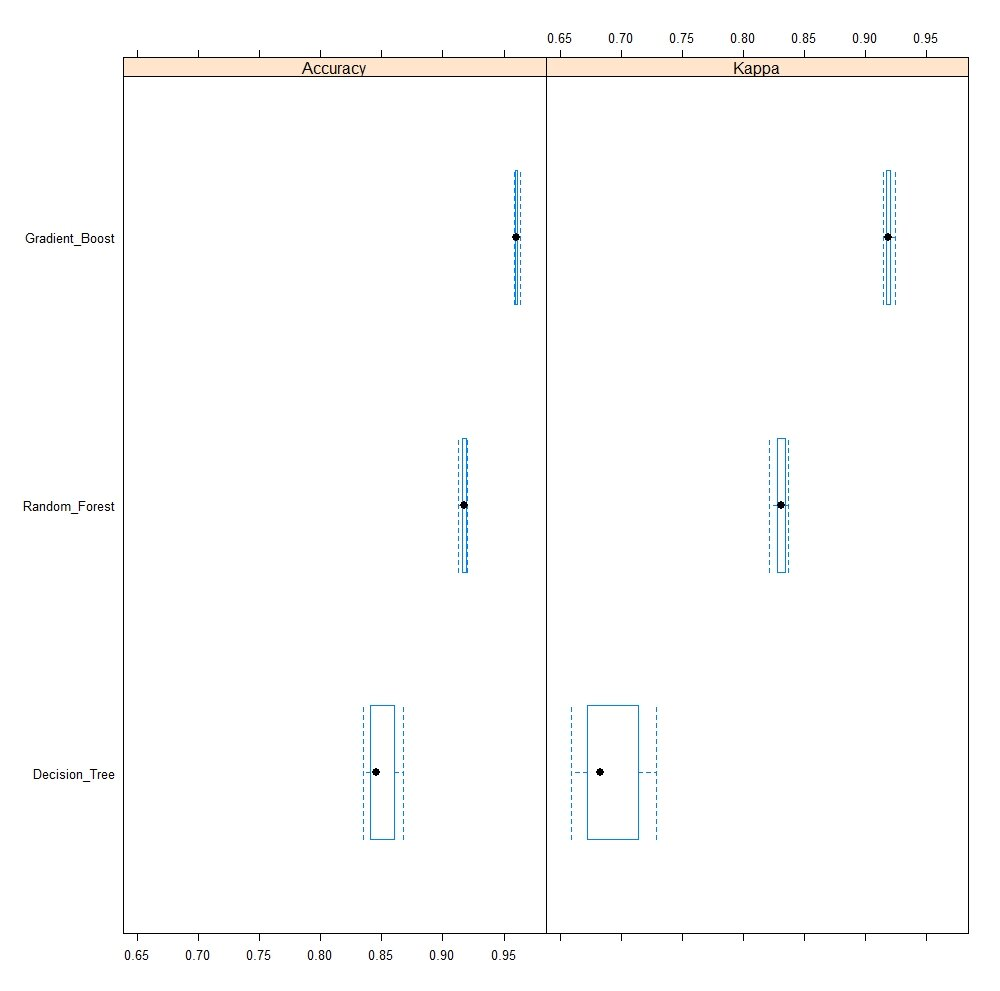
\includegraphics[width=.48\textwidth]{..//plots//boxplotcomparison.jpg}
  \caption{Left: Summary of the comparison, Right: Visualisation of the comparison}\label{fig:foobar}
\end{figure}

\end{document}
